% ecexpo_presentation.tex

% Copyright 2019 Clara Eleonore Pavillet

% Author: Clara Eleonore Pavillet
% Description: This is an unofficial Oxford University Beamer Template I made from scratch. Feel free to use it, modify it, share it.
% Version: 1.0

\documentclass{beamer}
\usepackage{import} % for some reason, this doesn't work when called in sty file
% Load Packages
\usepackage[utf8]{inputenc}
\usepackage{xcolor}
\usepackage{tikz}
\usetikzlibrary{positioning,calc}
\usepackage{graphicx}
\usepackage{hyperref}
\usepackage{amsmath}
\usepackage{listings}
\usepackage{fontawesome}

% Define Commands
\newcommand*{\ClipSep}{0.06cm} %To adjust footer logo
\newcommand{\E}{\mathrm{e}\,} %\def\I{e} % used to defined e for exp(x), see later what it should be
\newcommand{\ud}{\mathrm{d}}
\lstset{numbers=left, numberstyle=\tiny, stepnumber=1,firstnumber=1,breaklines=true,
    numbersep=5pt,language=Python,
    stringstyle=\ttfamily,
    basicstyle=\footnotesize, 
    showstringspaces=false
}

\usepackage{lecture_notes}
\usepackage{bibentry}
\usepackage[utf8]{inputenc}
\usepackage[T1]{fontenc}
\usepackage{algorithm}
\usepackage{algpseudocode}

\newcommand{\nn}{\nonumber}
\newcommand{\var}{\sigma^2}
\newcommand{\Rho}{\mathrm{P}}
\newcommand{\Tr}{\mathrm{Tr}} 
\newcommand{\diag}{\mathrm{diag}} 
%\DeclareMathOperator{\Tr}{Tr}
% \newcommand{\E}{\mathrm{E}}
\newcommand{\Prob}{\mathrm{Pr}}
% Theorems
\newtheorem{myth}{Theorem}
\newtheorem{mypro}{Proposition}
\newtheorem{mylem}{Lemma}
\newtheorem{mycor}{Corollary}
% Sets
\newcommand{\R}{\mathbb R}
% \newcommand{\I}{\mathbb I}
\newcommand{\C}{\mathbb C}
\newcommand{\Z}{\mathbb Z}
\newcommand{\BBE}{\mathbb E}
% Vectors
\newcommand{\av}{{\bf a}}
\newcommand{\bv}{{\bf b}}
\newcommand{\cv}{{\bf c}}
\newcommand{\dv}{{\bf d}}
\newcommand{\ev}{{\bf e}}
\newcommand{\fv}{{\bf f}}
\newcommand{\gv}{{\bf g}}
\newcommand{\hv}{{\bf h}}
\newcommand{\iv}{{\bf i}}
\newcommand{\jv}{{\bf j}}
\newcommand{\kv}{{\bf k}}
\newcommand{\lv}{{\bf l}}
\newcommand{\mv}{{\bf m}}
\newcommand{\nv}{{\bf n}}
\newcommand{\ov}{{\bf o}}
\newcommand{\pv}{{\bf p}}
\newcommand{\qv}{{\bf q}}
\newcommand{\rv}{{\bf r}}
\newcommand{\sv}{{\bf s}}
\newcommand{\tv}{{\bf t}}
\newcommand{\uv}{{\bf u}}
\newcommand{\wv}{{\bf w}}
\newcommand{\vv}{{\bf v}}
\newcommand{\xv}{{\bf x}}
\newcommand{\yv}{{\bf y}}
\newcommand{\zv}{{\bf z}}
\newcommand{\zerov}{{\bf 0}}
\newcommand{\onev}{{\bf 1}}
% Matrices
\newcommand{\Am}{{\bf A}}
\newcommand{\Bm}{{\bf B}}
\newcommand{\Cm}{{\bf C}}
\newcommand{\Dm}{{\bf D}}
\newcommand{\Em}{{\bf E}}
\newcommand{\Fm}{{\bf F}}
\newcommand{\Gm}{{\bf G}}
\newcommand{\Hm}{{\bf H}}
\newcommand{\Id}{{\bf I}}
\newcommand{\Jm}{{\bf J}}
\newcommand{\Km}{{\bf K}}
\newcommand{\Lm}{{\bf L}}
\newcommand{\Mm}{{\bf M}}
\newcommand{\Nm}{{\bf N}}
\newcommand{\Om}{{\bf O}}
\newcommand{\Pm}{{\bf P}}
\newcommand{\Qm}{{\bf Q}}
\newcommand{\Rm}{{\bf R}}
\newcommand{\Sm}{{\bf S}}
\newcommand{\Tm}{{\bf T}}
\newcommand{\Um}{{\bf U}}
\newcommand{\Wm}{{\bf W}}
\newcommand{\Vm}{{\bf V}}
\newcommand{\Xm}{{\bf X}}
\newcommand{\Ym}{{\bf Y}}
\newcommand{\Zm}{{\bf Z}}
% Calligraphic
\newcommand{\Ac}{{\cal A}}
\newcommand{\Bc}{{\cal B}}
\newcommand{\Cc}{{\cal C}}
\newcommand{\Dc}{{\cal D}}
\newcommand{\Ec}{{\cal E}}
\newcommand{\Fc}{{\cal F}}
\newcommand{\Gc}{{\cal G}}
\newcommand{\Hc}{{\cal H}}
\newcommand{\Ic}{{\cal I}}
\newcommand{\Jc}{{\cal J}}
\newcommand{\Kc}{{\cal K}}
\newcommand{\Lc}{{\cal L}}
\newcommand{\Mc}{{\cal M}}
\newcommand{\Nc}{{\cal N}}
\newcommand{\Oc}{{\cal O}}
\newcommand{\Pc}{{\cal P}}
\newcommand{\Qc}{{\cal Q}}
\newcommand{\Rc}{{\cal R}}
\newcommand{\Sc}{{\cal S}}
\newcommand{\Tc}{{\cal T}}
\newcommand{\Uc}{{\cal U}}
\newcommand{\Wc}{{\cal W}}
\newcommand{\Vc}{{\cal V}}
\newcommand{\Xc}{{\cal X}}
\newcommand{\Yc}{{\cal Y}}
\newcommand{\Zc}{{\cal Z}}


\def\E{\textrm{E}}

\newcommand{\boldeta}{\boldsymbol{\eta}}
\graphicspath{ {../images/} }

\nobibliography*
% \usepackage[perpage]{footmisc}
\usetheme{oxonian}

\newcommand{\fignocap}[2]{
	\begin{figure}[!hbtp]
	    \centering
		\includegraphics[width=#1\linewidth]{#2}
	\end{figure}
}

\newcommand{\subfignocap}[5]{
  \begin{figure}[!hbtp]
      \centering
    \subfigure{\includegraphics[width=#1\linewidth]{#2}}
    \hspace{#5}%
    \subfigure{\includegraphics[width=#3\linewidth]{#4}}
  \end{figure}
}

% vec
\renewcommand{\vec}[1]{\mathbf{#1}}

% MSE
\newcommand{\mse}[1]{\text{MSE}\left({#1}\right)}

% https://tex.stackexchange.com/questions/434931/reorder-note-field-at-the-end-of-the-reference
% \DeclareSourcemap{
%   \maps[datatype=bibtex]{
%     \map[overwrite=false]{
%       \step[fieldsource=note]
%       \step[fieldset=addendum, origfieldval, final]
%       \step[fieldset=note, null]
%     }
%   }
% }

\title{Efficient Deep Learning for Massive MIMO Channel State Estimation}
\titlegraphic{
\includegraphics[width=3cm]{Theme/Logos/DavisLogoV1.png}}
\author{\small{Mason del Rosario}}
\institute{Doctoral Exit Seminar}
\date{September 2022} %\today

\begin{document}
% \bibliographystyle{ieeetr}
% \nobibliography*{refs}


{\setbeamertemplate{footline}{} 
\frame{\titlepage}}

\section*{Outline}\begin{frame}{Outline}\tableofcontents\end{frame}

\section{Background}

  % Background section frame 
  \begin{frame}[plain]
    \vfill
    \centering
    \begin{beamercolorbox}[sep=8pt,center,shadow=true,rounded=true]{Background}
      \usebeamerfont{title}\insertsectionhead\par%
      \color{davisblue}\noindent\rule{10cm}{1pt} \\
      % \LARGE{\faFileTextO}
      \footnotesize{Feedback-based estimation of channel state information in MIMO networks.}
    \end{beamercolorbox}
    \vfill
    \begin{figure}[htb]
      \centering
      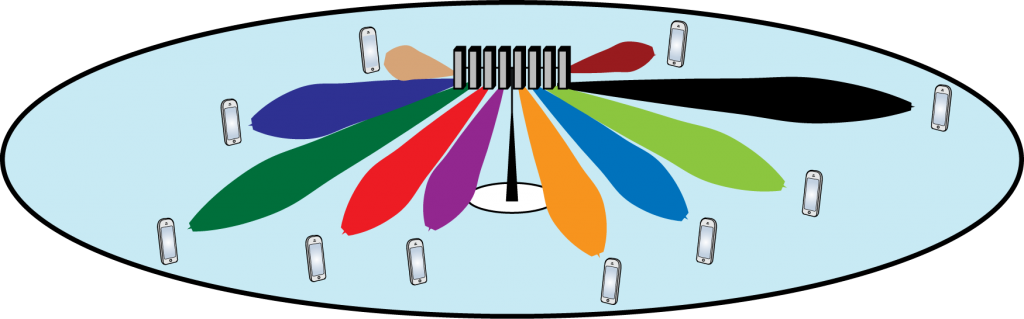
\includegraphics[width=.8\textwidth]{mimo-downlink.png} % https://ma-mimo.ellintech.se/what-is-massive-mimo/
      \medskip
      % \caption{Magnitude of spatial-frequency ($\bar{\mathbf H}$) and angular-delay ($\mathbf H$) CSI matrices.}
      % \label{fig:freq-vs-delay}
    \end{figure}
  \end{frame}

\subsection{Role of CSI in MIMO}

 %  \nofoot{
	% \begin{frame}{Why MIMO?}
	% 	Massive MIMO is a key enabling technology for future wireless communications networks.
	% 	\begin{itemize}
	% 		\item 5G, Ultra-Dense Networks, IoT
	% 	\end{itemize}
	% 	\pause
	% 	The efficacy of MIMO depends on accurate \emph{Channel State Information (CSI)}.
 %    \blfootnote{S. Marek, ``Sprint Spent \$1B on Massive MIMO for Its 5G Network in Q2," \emph{SDxCentral}, \url{https://www.sdxcentral.com/articles/news/sprint-spent-1b-on-massive-mimo-for-its-5g-network-in-q2/2018/06/}. Accessed: Feb 22, 2020.}
	% \end{frame}
 %  }

  \nofoot{
  \begin{frame}{MIMO and CSI}
    % Massive MIMO uses numerous antennas to endow transceivers with spatial diversity.
    % \fignocap{0.8}{mimo-nopre.PNG}
    \begin{columns}
      \begin{column}{0.5\linewidth}
        \begin{figure}[!hbtp]
        \centering
        {
          \fontsize{4pt}{8pt}
          \def\svgwidth{\columnwidth}
          \input{../images/mimo-diagram.pdf_tex}
        }
        % \caption{Multi-antenna transmitter (BS, gNB) and single-antenna user equipment (UE) with relevant system values.}
        % \label{fig:tdd_fdd}
        \end{figure}
      \end{column}
      \begin{column}{0.5\linewidth}
      \begin{itemize}
        \item MIMO = Multiple input multiple output
        \pause
        \item Massive w.r.t. antenna count, not physical size.
        \pause
        \item Spatial diversity $\to$ \textbf{high throughput}. 
      \end{itemize}
      \end{column}
    \end{columns}
    \blfootnote{\bibentry{ref:Bjornson2016MIMOMyths}}
  \end{frame}
  }

	\begin{frame}{MIMO and CSI} 
		% \fignocap{0.8}{mimo-nopre.PNG}
    \begin{figure}[!hbtp]
    \centering
    {
      \fontsize{4pt}{8pt}
      \def\svgwidth{0.9\columnwidth}
      \input{../images/mimo-schematic.pdf_tex}
    }
    \caption{Multi-antenna transmitter (BS, gNB) and single-antenna user equipment (UE) with relevant system values.}
    \label{fig:mimo_schematic}
    \end{figure}
	\end{frame}

	\begin{frame}{MIMO and CSI}
		In OFDM, the fading coefficients between Tx/Rx $=$ \textbf{Channel State Information (CSI)}, $\bar{\mathbf{H}}$. 
		\begin{align*}
			\bar{\mathbf{H}}&=\begin{bmatrix}
                          % h_{1,1} & h_{1,2} & \dots  & h_{1,N_b} \\
                          % h_{2,1} & h_{2,2} & \dots  & h_{2,N_b} \\
                          % \vdots  & \vdots  & \vdots & \vdots    \\
                          % h_{N_{f},1} & h_{N_{f},2} & \dots  & h_{N_{f},N_b} \\
            							h_{1,1} & h_{1,2} & \dots  & h_{1,N_f} \\
            							h_{2,1} & h_{2,2} & \dots  & h_{2,N_f} \\
            							\vdots	& \vdots  & \vdots & \vdots    \\
            							h_{N_{b},1} & h_{N_{b},2} & \dots  & h_{N_{b},N_f} \\
            						\end{bmatrix}
                        % \in \mathbb C^{N_f \times N_b}
                        \in \mathbb C^{N_b \times N_f}
		\end{align*}
    For $N_b$ transmit antennas and $N_f$ subcarriers.
	\end{frame}

  \begin{frame}{MIMO and CSI}
    % Massive MIMO uses numerous antennas to endow transceivers with spatial diversity.
    Downlink-uplink reciprocity in TDD, but not in FDD.
    % \fignocap{0.8}{mimo-nopre.PNG}
    \begin{figure}[!hbtp]
    \centering
    {
      \fontsize{4pt}{8pt}
      \def\svgwidth{0.9\columnwidth}
      \input{../images/tdd_fdd.pdf_tex}
    }
    % \caption{Multi-antenna transmitter (BS, gNB) and single-antenna user equipment (UE) with relevant system values.}
    % \label{fig:tdd_fdd}
    \end{figure}
    \pause
    FDD requires feedback for downlink CSI estimation.
  \end{frame}

  \begin{frame}{MIMO and CSI}
    Transmitting $\bar{\mathbf{H}}$ is costly. Instead, generate estimates, $\hat{\bar{\mathbf{H}}}$, based on \textbf{compressed feedback}, $\mathbf z$.\\
    \vspace{24pt}
    \begin{figure}[!hbtp]
    \centering
    {
      \fontsize{4pt}{6pt}
      \def\svgwidth{0.9\columnwidth}
      \input{../images/mimo-schematic-feedback.pdf_tex}
    }
    % \caption{Example multi-antenna transmitter (BS, gNB) and single-antenna user equipment (UE) and relevant system values.}
    % \label{fig:mimo_schematic_feedback}
    \end{figure}
  \end{frame}

	% \begin{frame}{MIMO and Perfect CSI}
	% 	\textbf{Perfect CSI} (i.e., exact knowledge of the channel, $\mathbf{H}$) allows us to maximize the power of the received symbol by precoding.

	% 	\fignocap{0.8}{mimo-pre.PNG}
	% \end{frame}

	% \begin{frame}{MIMO and CSI Estimation}
	% 	However, transmitting $\mathbf{H}$ is costly. Instead, generate \textbf{CSI Estimates}, $\hat{\mathbf{H}}$, based on \textbf{compressed feedback}.\\
	% 	\fignocap{0.8}{mimo-feed.PNG}
 %    \textbf{Goal}: Find low-dimensional representation, feed back to transmitter for recovery of $\hat{\mathbf{H}}$ which is an accurate approximation of $\mathbf{H}$ in MSE sense. % add something about need fro compression
	% \end{frame}

  \nofoot{
  \begin{frame}{CSI Sparsity}
      \footnotesize{ 
        Denote 2D inverse FFT of $\bar{\mathbf H}$ as
       \begin{align*}
       \tilde{\mathbf H} = \mathbf F^H\bar{\mathbf H}\mathbf F.
       \end{align*}
        % While $\bar{\mathbf H}$ is used for beamforming, $\mathbf H$ is more amenable to compression.
      }
      \begin{figure}[htb]
        \centering
        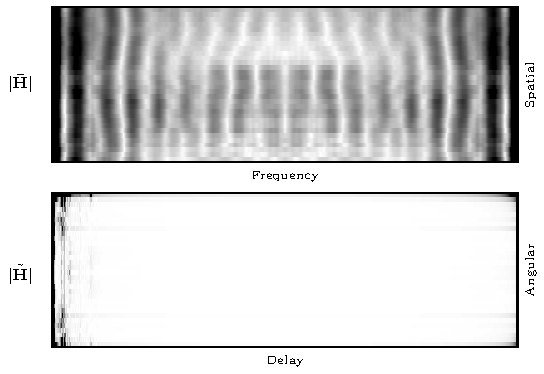
\includegraphics[width=.8\textwidth]{batch17_sample0.pdf}
        \medskip
        % \caption{Magnitude of spatial-frequency ($\bar{\mathbf H}$) and angular-delay ($\mathbf H$) CSI matrices.}
        % \label{fig:freq-vs-delay}
      \end{figure}
  \end{frame}
  }

  \nofoot{
  \begin{frame}{CSI Sparsity}
      \footnotesize{ 
        Given sparsity of $\tilde{\mathbf H}$, we can encode/decode a truncated version, $\mathbf H$.
      }
      \begin{figure}[htb]
        \centering
        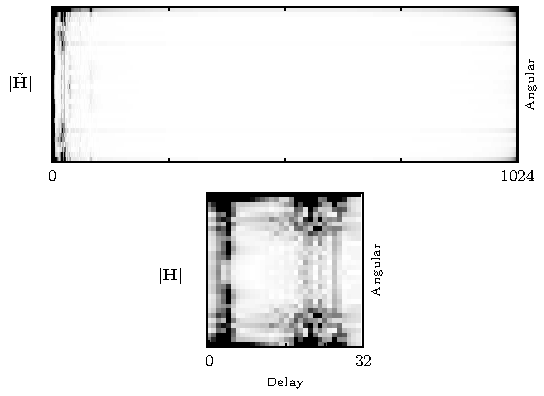
\includegraphics[width=.8\textwidth]{batch17_sample0_truncatevsfull.pdf}
        \medskip
        % \caption{Magnitude of spatial-frequency ($\bar{\mathbf H}$) and angular-delay ($\mathbf H$) CSI matrices.}
        % \label{fig:freq-vs-delay}
      \end{figure}
  \end{frame}
  }

  \subsection{CSI Estimation}

    \begin{frame}{CSI Estimation Methods}
       \begin{enumerate}
       \item Compressed Sensing (Conventional)
       \item Convolutional Neural Networks (This proposal)
      \end{enumerate} 
    \end{frame}

  \subsubsection{Compressed Sensing}

    \nofoot{
    \begin{frame}{Compressed Sensing}
    \footnotesize{
      Find low-dimensional basis for sparse data, $\mathbf h$,
      \begin{align*}
        \mathbf{y}&=\mathbf A\mathbf{h} + \mathbf{n}.
      \end{align*}
      % s.t. $\mathbf{h}=$ vectorized CSI measurement, $\mathbf A=$ the measurement matrix, and $\mathbf n=$ additive noise.
      \begin{figure}[!hbtp] \centering 
        % \includegraphics[width=0.46\textwidth]{images/nmse_indoor_mag.eps}
        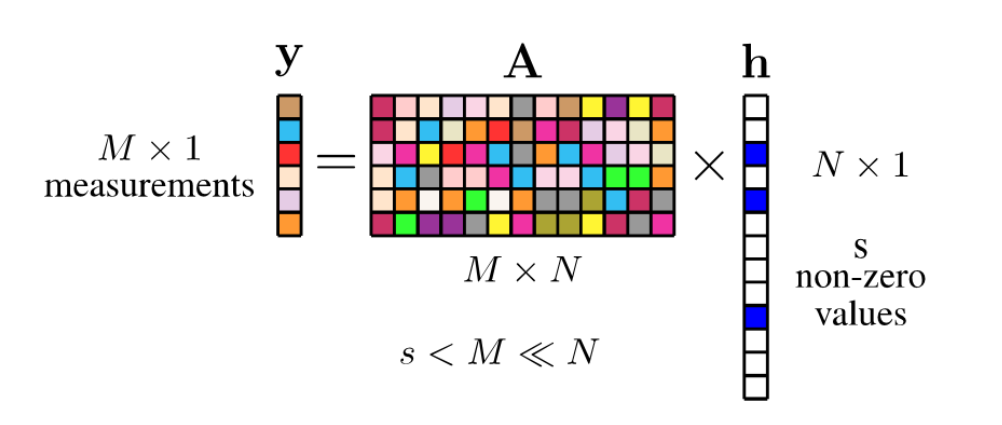
\includegraphics[width=0.65\textwidth]{cs-measurement.png}
        % \caption{Random measurement matrix $\mathbf A$, additive noise $\mathbf n$.} % (from \cite{ref:Marques2019ReviewOfSparseRecovery}). 
        \label{fig:cs-measurement} \vspace*{-2mm}
      \end{figure}
      % \textbf{Problems:} Strong sparsity assumptions, not necessarily true in real-world data. Iterative algorithms = computationally expensive.
      \blfootnote{\bibentry{ref:Marques2019ReviewOfSparseRecovery}}
      }
    \end{frame}
    }    

    \nofoot{
    \begin{frame}{Compressed Sensing}
    \footnotesize{
      CS addresses two major issues:
      \begin{enumerate}
        \item Design of $\mathbf A$ (stochastic or deterministic).
        \pause
        % \item Recovery of $\hat{\mathbf h}$ given $\mathbf A$ and $\mathbf y$ (e.g., Orthogonal Matching Pursuit \cite{ref:Marques2018CSForWidebandHFChannelEstimation}).
        \item Recovery of $\hat{\mathbf h}$ given $\mathbf A$ and $\mathbf y$, typically via convex optimization on $p$-norm minimization,
        \begin{align*}
          \min \|\hat{\mathbf h}\|_p \; \text{subject to} \; \|\mathbf{y}-\mathbf A\hat{\mathbf h}\|_2^2 < \epsilon.
        \end{align*}
      \end{enumerate} 
      % \blfootnote{\bibentry{ref:Marques2018CSForWidebandHFChannelEstimation}}
      \pause
      \textbf{Problems:} 
      \begin{itemize} 
        \item Recovery algorithms are iterative.
        \pause
        \item Complexity scales with sparsity ($M\propto s$).
      \end{itemize}
    }
    \end{frame}
    }


  \subsubsection{Convolutional Neural Networks}

    \nofoot{
    \begin{frame}{Convolutional Neural Networks (CNNs)}
      \begin{itemize}
        % \item Capable of extracting features from 2D, grid-like data 
        \item Layers of trainable linear functions followed by nonlinear ‘activation’ functions.
        \item State-of-the art performance in image processing
        \fignocap{0.35}{filt1.JPEG}
        \pause
        \item No assumptions on sparsity/RIP. Instantaneous decoding.
      \end{itemize}
      \blfootnote{A. Karpathy, ``Visualizing What ConvNets Learn,"  \url{http://cs231n.github.io/understanding-cnn/}. Accessed: Feb 24, 2020.}
    \end{frame}
    }

    \nofoot{
    \begin{frame}{CNN Autoencoder}
    \footnotesize{
      \textbf{Autoencoder}: Estimate $\hat{\mathbf H}$, latent code $\mathbf Z$ with \textbf{compression ratio},
      \begin{align*} 
        \text{CR} = \frac{\text{dim}(\mathbf Z)}{\text{dim}(\mathbf H)} \; \text{s.t.} \;\text{dim}(\mathbf Z) < \text{dim}(\mathbf H).
      \end{align*}
      \begin{figure}[!hbtp]
      \centering
      \fontsize{6pt}{8pt}
      \def\svgwidth{0.6\columnwidth}
      \input{../images/autoencoder_schematic.pdf_tex}
      % \caption{Abstract schematic for an autoencoder operating on CSI matrices $\mathbf H$. The encoder learns a latent representation, $\mathbf Z$, while the decoder learns to reconstruct estimates $\hat{\mathbf H}$.}
      % \label{fig:autoencoder_schematic}
      \end{figure}
      \pause
      $\theta_e, \theta_d$ updated to minimize \textbf{mean-squared error (MSE)},
      \begin{align*}
      \underset{\theta_e, \theta_d}{\text{argmin}}\; \frac 1N \sum_{i=1}^N\Arrowvert \mathbf H_i - g(f(\mathbf H_i, \theta_e), \theta_d) \Arrowvert^2.
      \end{align*}
      }
    \end{frame}
    }

    \nofoot{
    \begin{frame}{CsiNet}
      \begin{itemize}
        \item CNN autoencoder for learned CSI compression and feedback \cite{ref:csinet}
        % \item Expanded their work to use Recurrent Neural Networks \cite{ref:Wang2019CsiNetLSTM}
      \end{itemize}
      \fignocap{0.9}{csinet-fig-paper.PNG}
      % [3] CsiNet paper
      % [4] CsiNet-LSTM paper
      \blfootnote{\bibentry{ref:csinet}}
    \end{frame}
    }

    \nofoot{
    \begin{frame}{CsiNet vs. Compressed Sensing}
      \footnotesize{CNNs outperform CS at comparable compression ratios.}
      \fignocap{0.5}{csinet-results.PNG}
      \blfootnote{\bibentry{ref:csinet}}
    \end{frame}
    }

    \nofoot{
    \begin{frame}{CsiNet vs. Compressed Sensing}
      \begin{figure}
        \centering
        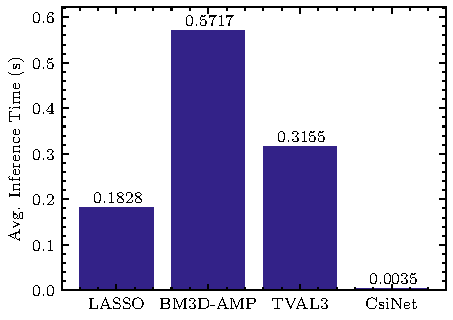
\includegraphics[width=0.7\linewidth]{csinet-vs-cs-timing.pdf}
        \caption{Average inference time for compressed sensing methods vs. CsiNet.}
      \end{figure}
      \blfootnote{\bibentry{ref:csinet}}
    \end{frame}
    }

  \nofoot{
  \begin{frame}{Domain Knowledge + CNNs for CSI Estimation}
    \begin{figure}[htb] \centering 
      % 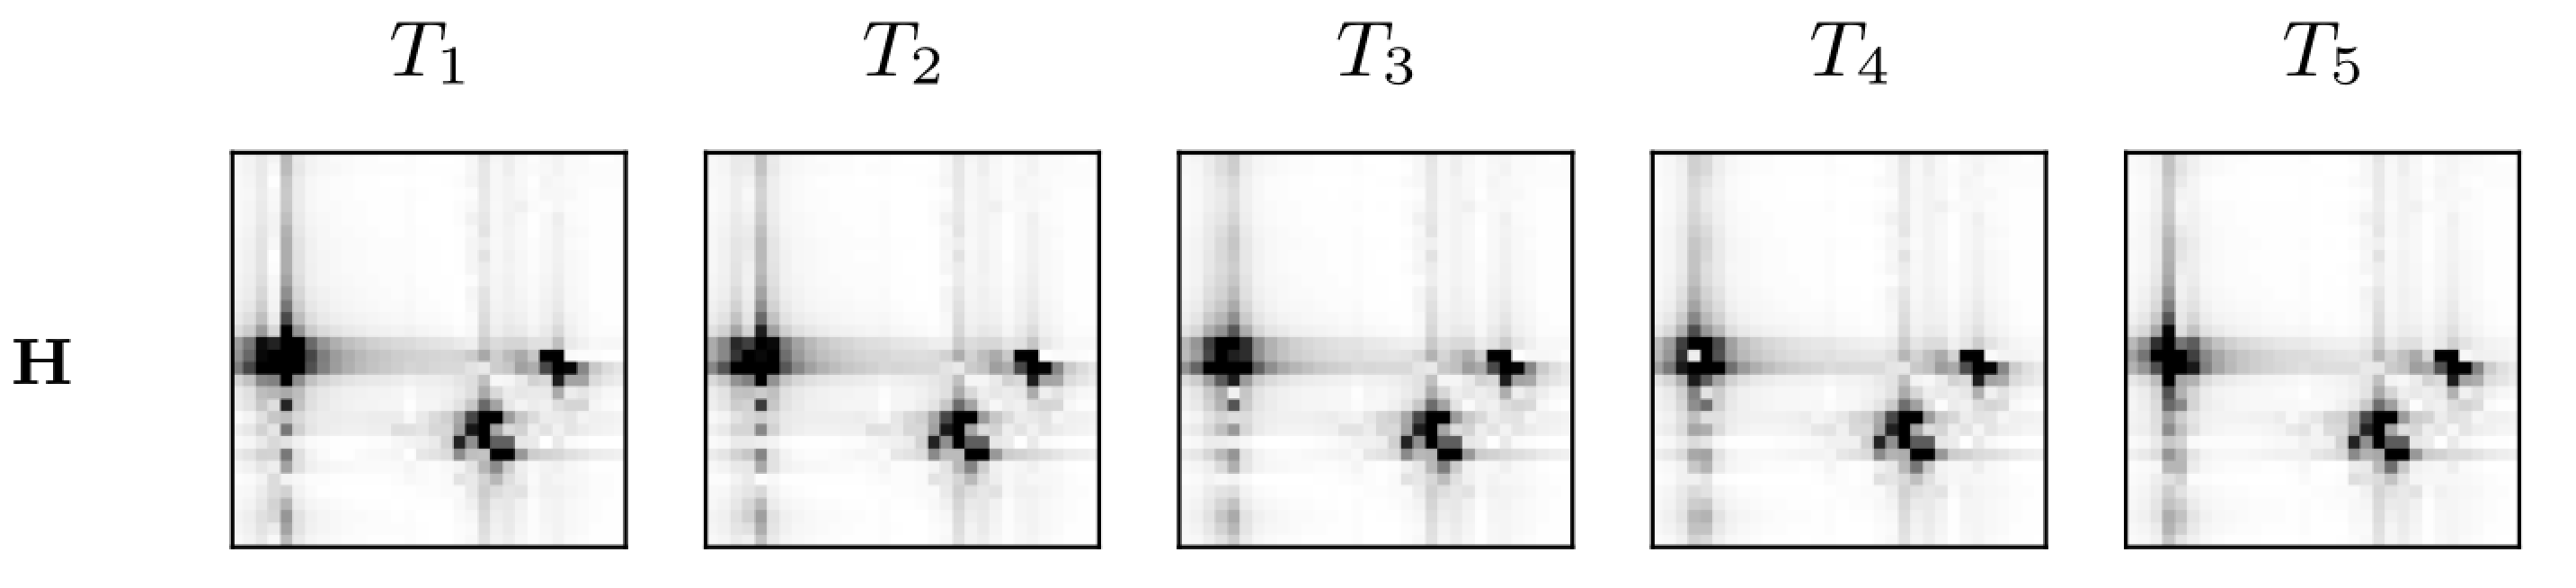
\includegraphics[width=0.9\linewidth]{batch0_csi_gt.png}
    {
      \fontsize{4pt}{4pt}
      \def\svgwidth{\columnwidth}
      \input{../images/cnns-venn-diagram-contrib-final.pdf_tex}
    }
    \caption{Areas of \emph{domain knowledge} and corresponding CNNs.}
    \end{figure}
  \end{frame}
  }

\section{Completed Work \#1: SphNet}

  % Spherical Normalization section frame 
  \begin{frame}[plain]
    \vfill
    \centering
    \begin{beamercolorbox}[sep=8pt,center,shadow=true,rounded=true]{Spherical Normalization}
      \usebeamerfont{title}\insertsectionhead\par%
      \color{davisblue}\noindent\rule{10cm}{1pt} \\
      % \vspace{8pt}
      \footnotesize{Power-based normalization for improved CSI reconstruction accuracy.}
      % \LARGE{\faFileTextO}
    \end{beamercolorbox}
    \vfill
  \end{frame}

  \nofoot{
  \begin{frame}{CSI vs. Images: Channels}
    \begin{figure}[htb]    
      {
        \fontsize{8pt}{8pt}
        \def\svgwidth{\columnwidth}
        \input{../images/datasets.pdf_tex}
      }
      % \caption{Distribution/variance of COST2100 real/imaginary channels under minmax normalization ($N=10^5$).}
      % \label{fig:cost_dist}
    \end{figure}
  \end{frame}
  }

  \nofoot{
  \begin{frame}{CSI vs. Images: CNNs}
    \begin{figure}[htb]    
      {
        \fontsize{10pt}{10pt}
        \def\svgwidth{\columnwidth}
        \input{../images/autoencoder_channels.pdf_tex}
      }
      % \caption{Distribution/variance of COST2100 real/imaginary channels under minmax normalization ($N=10^5$).}
      % \label{fig:cost_dist}
    \end{figure}
  \end{frame}
  }

  \nofoot{
  \begin{frame}{CsiNet: Minmax Normalization}
    \footnotesize{
    \begin{itemize}
      \item \textbf{Minmax normalization} -- Find minimum, maximum of channels.
      \pause
      \item $H_{n,(i,j)}=$ $(i,j)$-th element of $n$-th sample
      \begin{align*}
        H_{\text{minmax},n,(i,j)} &= \frac{H_{n,(i,j)}- H_{\text{min}}}{H_{\text{max}}- H_{\text{min}}} \in [0,1] 
        % &\forall \; n \in [1,\dots,N], i \in [1,\dots,R_d], j \in [1,\dots,N_f]
      \end{align*}
      \pause
      \item Compatible with common \textbf{activation functions} (e.g., tanh, sigmoid)
      % \item Makes data compatible with neural activation function (i.e., sigmoid)
    \end{itemize}
    }
    \begin{figure}[htb]
      \centering
      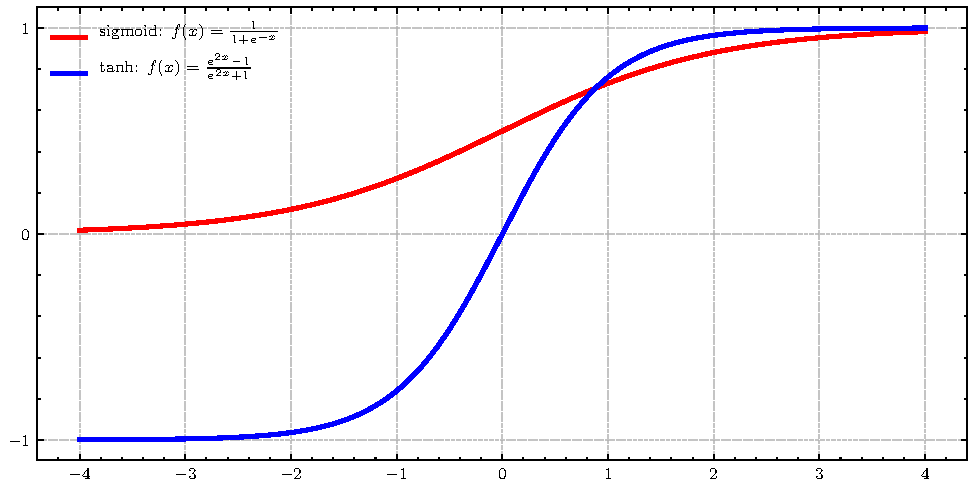
\includegraphics[width=.7\textwidth]{activations.pdf}
    \end{figure}
  \end{frame}
  }

  \nofoot{
  \begin{frame}{COST2100: Minmax Normalization}
    % Tanh normalization $\to$ larger variance. 
    \begin{figure}[htb]    
      \subfigure[Indoor] {\label{fig:dist_indoor} 
      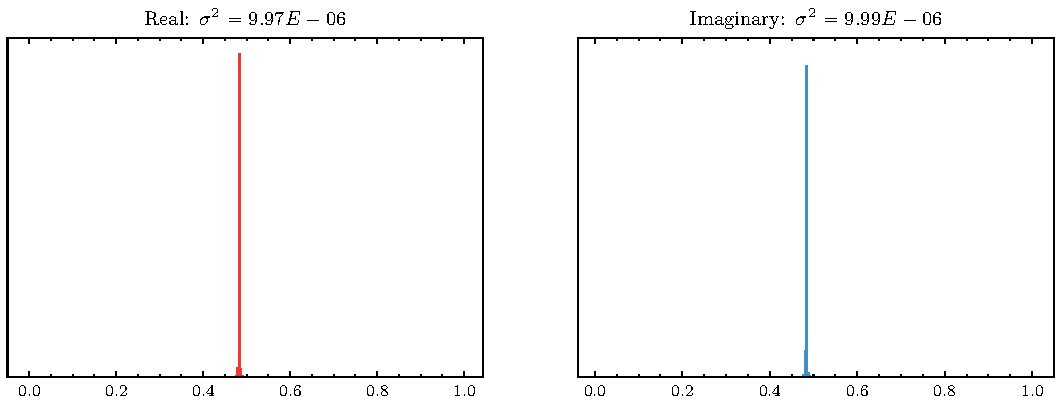
\includegraphics[width=.6\textwidth]{cost2100_indoor_dist.pdf}
      }
      \subfigure[Outdoor] {\label{fig:dist_outdoor} 
      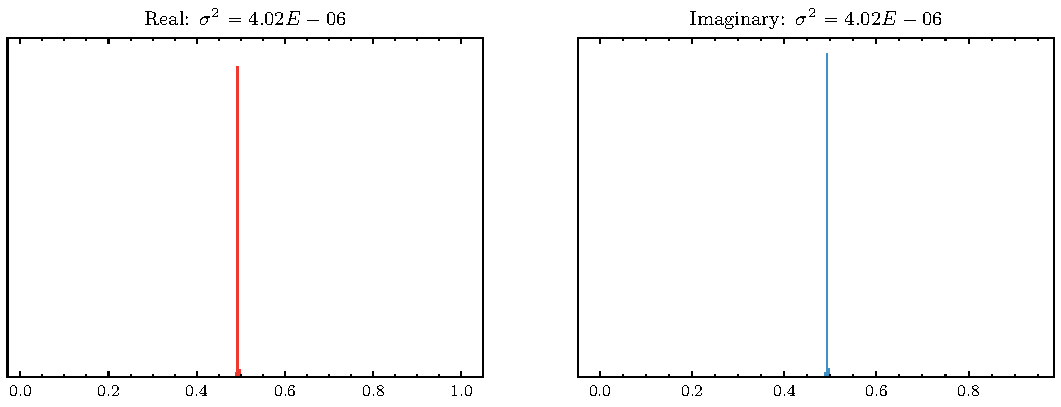
\includegraphics[width=.6\textwidth]{cost2100_outdoor_dist.pdf}
      }
      \caption{Distribution/variance of COST2100 real/imaginary channels under minmax normalization ($N=10^5$).}
      \label{fig:cost_dist}
    \end{figure}
  \end{frame} 
  }  

  \begin{frame}{ImageNet: Minmax Normalization}
    \begin{figure}[htb]
      \centering
      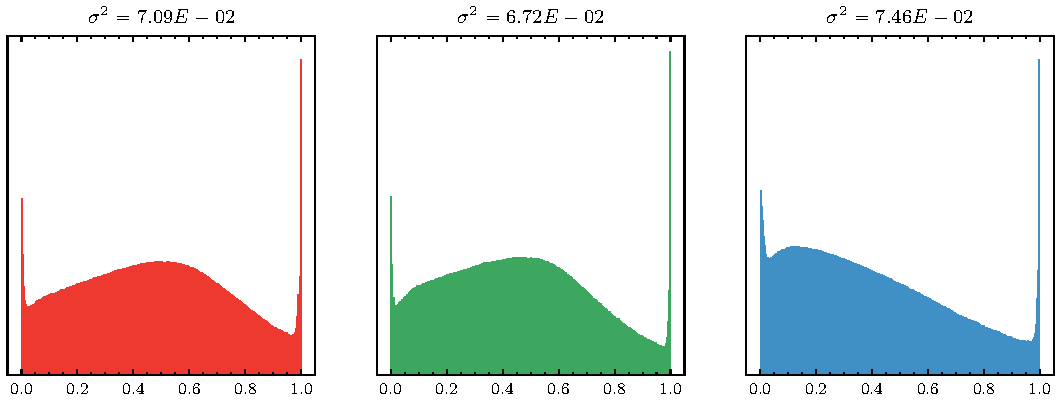
\includegraphics[width=.9\textwidth]{imagenet_rgb_dist.pdf}
      \medskip
      \caption{Distribution and variance of minmax-normalized ImageNet RGB channels ($N=50000$).}
      \label{fig:imagenet_dist}
    \end{figure}
  \end{frame}

  \begin{frame}{Comparison: Minmax Normalization}
    Difference of \textbf{four orders of magnitude}.
    \footnotesize{
    \begin{table}[htb]
      % \renewcommand{\arraystretch}{1.5}
      \begin{center}
        \begin{tabular}{|c|c|c|c|c|}
        \hline
        \textbf{Dataset} & \textbf{Env} & \textbf{Channels} & \textbf{Norm} & \textbf{Avg. Variance} \\ \hline
        ImageNet         & -            & RGB                 & Minmax                 & \underline{$7.09E^{-2}$}       \\ \hline
        COST2100         & Indoor       & Real, Imag          & Minmax                 & \underline{$9.98E^{-6}$}       \\ \hline          
        COST2100         & Outdoor      & Real, Imag          & Minmax                 & \underline{$4.02E^{-6}$}       \\ \hline
        \end{tabular}
        \caption{Minmax normalization applied to COST2100 and ImageNet dataset.}
        \label{tab:minmax-compare} 
      \end{center}
    \end{table}
    }
  \end{frame}

  % \nofoot{
  % \subsection{Bi-directional Reciprocity}
  % \begin{frame}{Bi-directional Reciprocity}
  %   \begin{columns}[T] % align columns
  %   \begin{column}{.48\textwidth}
  %   \begin{itemize}
  %     \item Goal = estimate downlink CSI
  %     \item In conventional CSI estimation for FDD, uplink is typically not used to estimate downlink
  %     \item With CNNs, can leverage correlation between uplink/downlink \cite{ref:dualnet}
  %   \end{itemize}
  %   \end{column}%
  %   \hfill%
  %   \begin{column}{.5\textwidth}
  %     \fignocap{0.9}{images/corr-fig.PNG}
  %   \end{column}%
  %   \end{columns}
  %   \blfootnote{\bibentry{ref:dualnet}}
  % \end{frame}
  % }

  % \begin{frame}{Bi-directional Reciprocity}
  %   \fignocap{1.0}{images/dualnet-fig.PNG}
  % \end{frame}

% \subsection{Spherical Normalization}
  \begin{frame}{Spherical Normalization}
    \textbf{Spherical normalization} -- scale $\mathbf H$ by power. For Frobenius norm $\|\cdot\|$,
    % TODO: Does this make sense? "For CSI matrices, we could choose to scale each element by it's mean and by the inverse covariance matrix."
    \begin{align}
      \mathbf{\check H}^n &= \frac{\mathbf H^n}{\|\mathbf H^n\|}. \label{eq:sph-intro}
    \end{align}
    Then apply minmax scaling to the entire dataset.
  \end{frame}

  \nofoot{
  \begin{frame}{COST2100: Spherical Normalization}
    % Tanh normalization $\to$ larger variance. 
    \begin{figure}[htb]    
      \subfigure[Indoor] {\label{fig:sph_dist_indoor} 
      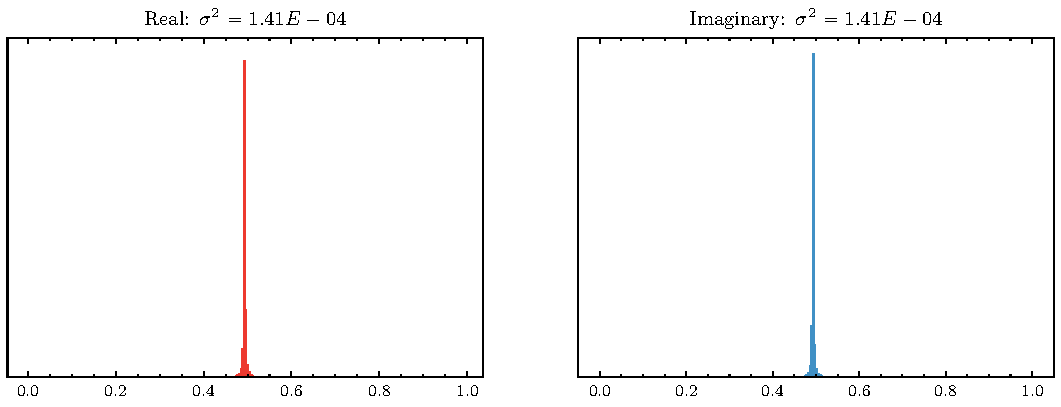
\includegraphics[width=.6\textwidth]{cost2100_indoor_sph_dist.pdf}
      }
      \subfigure[Outdoor] {\label{fig:sph_dist_outdoor} 
      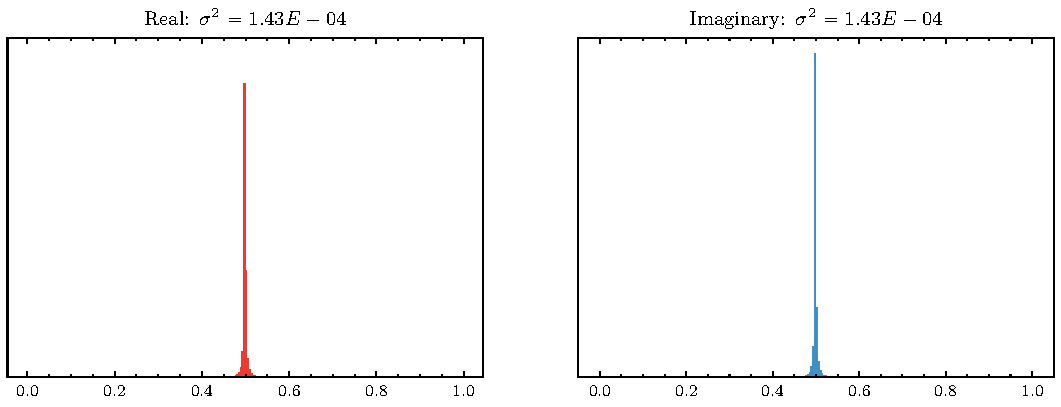
\includegraphics[width=.6\textwidth]{cost2100_outdoor_sph_dist.pdf}
      }
      \caption{Distribution/variance of COST2100 real/imaginary channels under spherical normalization ($N=10^5$).}
      \label{fig:cost_sph_dist}
    \end{figure}
  \end{frame} 
  }   

  % \begin{frame}{COST2100 (Indoor): Spherical Normalization}
  %   Spherical normalization $\to$ larger variance. 
  %   \begin{figure}[htb]
  %     \centering
  %     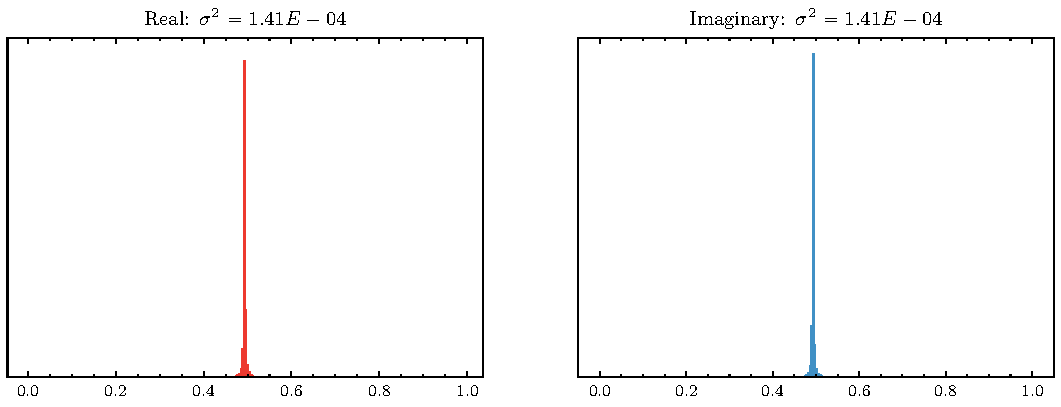
\includegraphics[width=.9\textwidth]{cost2100_indoor_sph_dist.pdf}
  %     % \medskip
  %     \caption{Distribution/variance of indoor COST2100 real/imaginary channels under spherical normalization ($N=99000$).}
  %     \label{fig:cost_indoor_sph_dist}
  %   \end{figure}
  % \end{frame}

    \begin{frame}{Comparison: Spherical vs. Minmax Normalization}
    Difference is now \textbf{two orders of magnitude}.
    \begin{table}[htb]
      % \renewcommand{\arraystretch}{1.5}
      \footnotesize{
      \begin{center}
        \begin{tabular}{|c|c|c|c|c|}
        \hline
        \textbf{Dataset} & \textbf{Env} & \textbf{Channels} & \textbf{Norm} & \textbf{Avg. Variance} \\ \hline
        ImageNet         & -                    & RGB                 & Minmax                 & \underline{$7.09E^{-2}$}       \\ \hline
        COST2100         & Indoor               & Real, Imag          & Spherical              & \underline{$1.41E^{-4}$}       \\ \hline
        COST2100         & Outdoor              & Real, Imag          & Spherical              & \underline{$1.43E^{-4}$}       \\ \hline
        COST2100         & Indoor               & Real, Imag          & Minmax                 & $9.98E^{-6}$       \\ \hline
        COST2100         & Outdoor              & Real, Imag          & Minmax                 & $4.02E^{-6}$       \\ \hline
        \end{tabular}
        \caption{Minmax vs. spherical normalization applied to COST2100 datasets compared with ImageNet.}
        \label{tab:minmax-sph-compare} 
      \end{center}
      }
    \end{table}
  \end{frame}

  % \begin{frame}{Comparison: Spherical vs. Minmax Normalization}
  %   Difference is now \textbf{two orders of magnitude}.
  %   \begin{table}[htb]
  %     % \renewcommand{\arraystretch}{1.5}
  %     \begin{center}
  %       \begin{tabular}{|c|c|c|c|}
  %       \hline
  %       \textbf{Dataset} & \textbf{Channels} & \textbf{Normalization} & \textbf{Avg. Variance} \\ \hline
  %       ImageNet       & RGB                 & Minmax                 & \underline{$7.24E^{-2}$}       \\ \hline
  %       COST2100       & Real, Imag          & Spherical              & \underline{$1.41E^{-4}$}       \\ \hline
  %       COST2100       & Real, Imag          & Minmax                 & $9.98E^{-6}$       \\ \hline
  %       \end{tabular}
  %       \caption{Minmax vs. spherical normalization applied to COST2100 datasets compared with ImageNet.}
  %       \label{tab:minmax-sph-compare} 
  %     \end{center}
  %   \end{table}
  % \end{frame}

  \begin{frame}{MSE/NMSE equivalence}
    \footnotesize{
    Spherical normalization $\to$ MSE equivalent to NMSE.
    \begin{align*}
      \text{MSE}=\frac 1N \sum_{k=1}^N\Arrowvert\mathbf H_k - \hat{\mathbf H}_k\Arrowvert^2,\quad \text{NMSE} =\frac 1N \sum_{k=1}^N\frac{\Arrowvert\mathbf H_k - \hat{\mathbf H}_k\Arrowvert^2}{\Arrowvert\mathbf H_k\Arrowvert} \\        
    \end{align*}
    \pause
    MSE of spherically normalized estimator yields,
    \begin{align*}
      \text{MSE}_{\text{Sph}} &= \frac 1N \sum_{k=1}^N\Arrowvert\check{\mathbf H}_k - \hat{\check{\mathbf H}}_k\Arrowvert^2 \\
      &= \frac 1N \sum_{k=1}^N\left\Arrowvert \frac{\mathbf H_k}{\Arrowvert\mathbf H_k\Arrowvert} - \frac{\hat{\mathbf H}_k}{\Arrowvert\mathbf H_k\Arrowvert}\right\Arrowvert^2 \\
      &= \frac 1N \sum_{k=1}^N\frac{\Arrowvert\mathbf H_k - \hat{\mathbf H}_k\Arrowvert^2}{\Arrowvert\mathbf H_k\Arrowvert}.
      % &= \text{NMSE} \; \Box
    \end{align*}
    }
\end{frame}
  % \begin{frame}{Spherical Normalization}
  %   CSI matrices are sparse in 2D (angular) delay domain.
  %   \begin{figure}[ht]
  %   \centering
  %   \incfig{csi-reshape}{0.75\columnwidth}
  %   % \caption{Pre-normalized data.}
  %   % \label{fig:csi-pre-norm}
  %   \end{figure}
  % \end{frame}

  % \begin{frame}{Spherical Normalization}
  %   CSI matrices are sparse in 2D (angular) delay domain.
  %   \begin{figure}[ht]
  %   \centering
  %   \incfig{csi-pre-norm}{0.75\columnwidth}
  %   % \caption{Pre-normalized data.}
  %   % \label{fig:csi-pre-norm}
  %   \end{figure}
  % \end{frame}

  % \begin{frame}{Spherical Normalization}
  %   Naive normalization of dataset, $\vec{H}$: cast all values to range [0,1] by scaling all entries by $\text{max}\left(\vec{H}\right)-\text{min}\left(\vec{H}\right)$.
  %   \begin{figure}[ht]
  %   \centering
  %   \incfig{csi-naive-norm}{0.75\columnwidth}
  %   % \caption{Pre-normalized data.}
  %   % \label{fig:csi-pre-norm}
  %   \end{figure}
  %   \pause
  %   \begin{itemize}
  %   \item Low-magnitude entries have less influence in updates during training.
  %   \end{itemize}
  % \end{frame}

  % \begin{frame}{Spherical Normalization}
  %   \textbf{Solution: Spherical normalization}. Scale each entry by sample power, $||\mathbf{H}_k||$. % Training data, $\check{\vec{H}}$, become
  %   \begin{figure}[ht]
  %   \centering
  %   \incfig{csi-sph-norm}{0.75\columnwidth}
  %   % \caption{Pre-normalized data.}
  %   % \label{fig:csi-pre-norm}
  %   \end{figure}
  %   \pause
  %   \begin{itemize}
  %   \item Low-magnitude entries maintain influence in updates during training.
  %   \end{itemize}
  %   % \begin{align*}
  %   %   \check{\vec{H}}^k = \frac{\vec{H}^k}{||\vec{H}^k||} 
  %   % \end{align*}
  %   % where $k$ denotes the $k-$th sample in the dataset. Compare with min-max training data, $\bar{\vec{H}}$,
  %   % \begin{align*}
  %   %   \bar{\vec{H}}^k = \frac{\vec{H}^k}{\text{max}\left(\vec{H}\right)-\text{min}\left(\vec{H}\right)} 
  %   % \end{align*}
  % \end{frame}

  \nofoot{
  \begin{frame}{SphNet Architecture}
    % \fignocap{0.9}{sphnet-fig.PNG}
    \begin{figure}[htb]
      \centering
      {
        \fontsize{1pt}{1pt}
        \def\svgwidth{1.0\columnwidth}
        \input{../images/csinet-pro.pdf_tex}
      }
      % 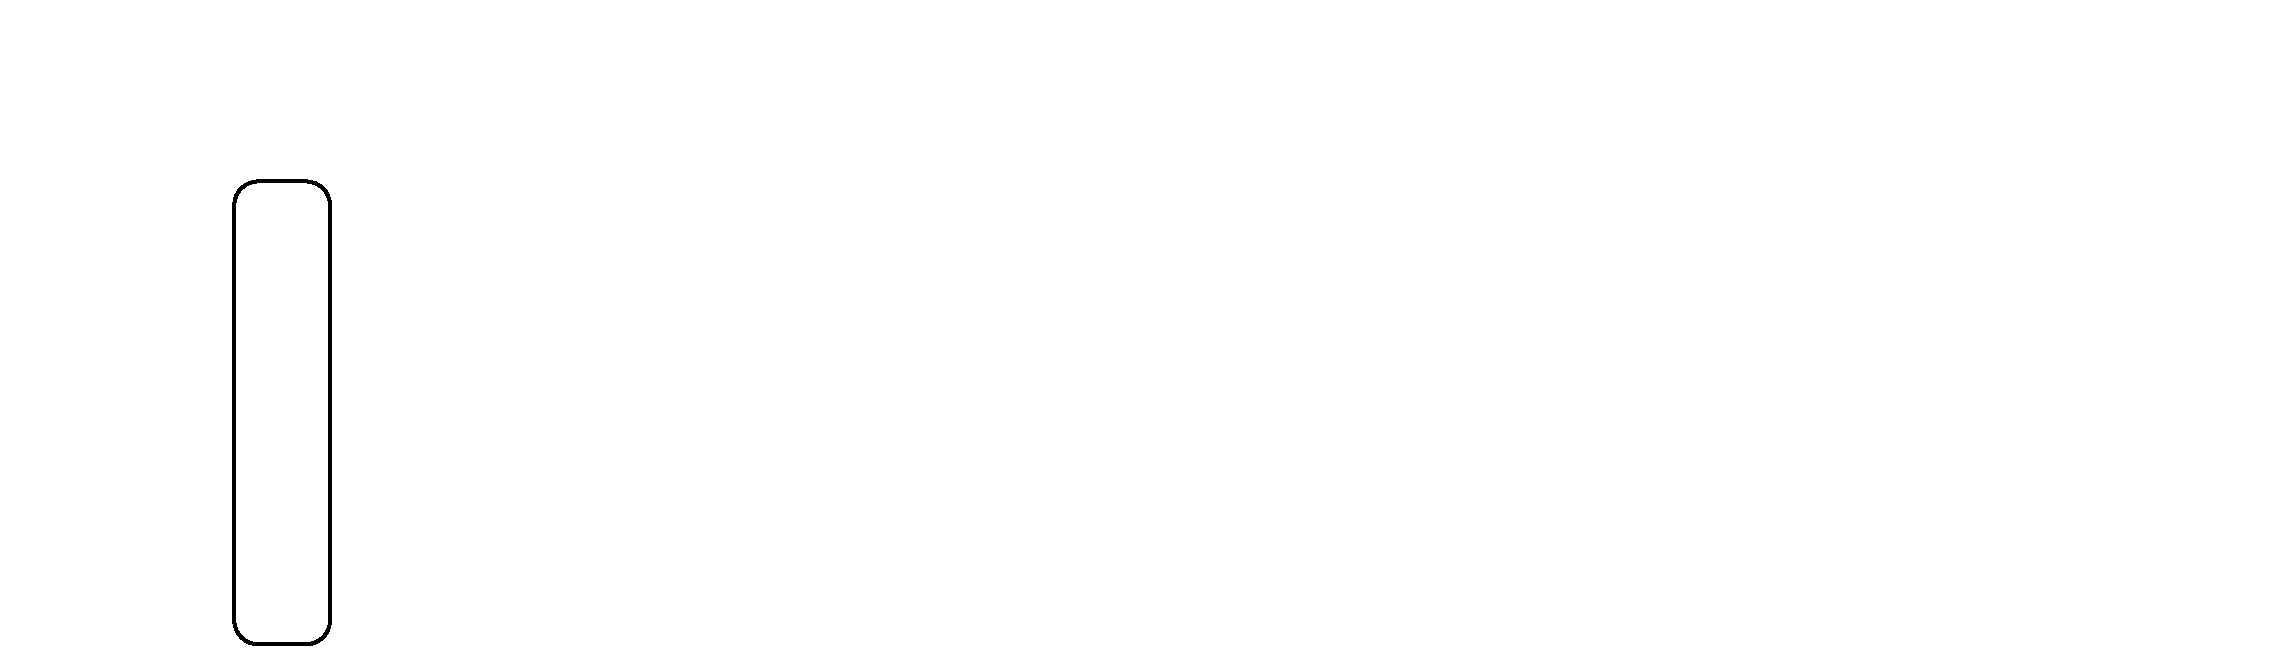
\includegraphics[width=.9\textwidth]{csinet-pro.pdf}
      % \medskip
      \caption{SphNet -- CsiNetPro architecture with Spherical Normalization.}
      \label{fig:sphnet-arch}
    \end{figure}
  \blfootnote{\bibentry{ref:liu2020sphnet}}
  \end{frame}  
  }

  % dualnet arch
  % \nofoot{
  % \begin{frame}{DualNet-Sph Architecture}
  %   % \fignocap{0.9}{sphnet-fig.PNG}
  %   \begin{figure}[htb]
  %     \centering
  %     {
  %       \fontsize{1pt}{1pt}
  %       \def\svgwidth{1.0\columnwidth}
  %       \input{../images/dualnet-pro.pdf_tex}
  %     }
  %     % 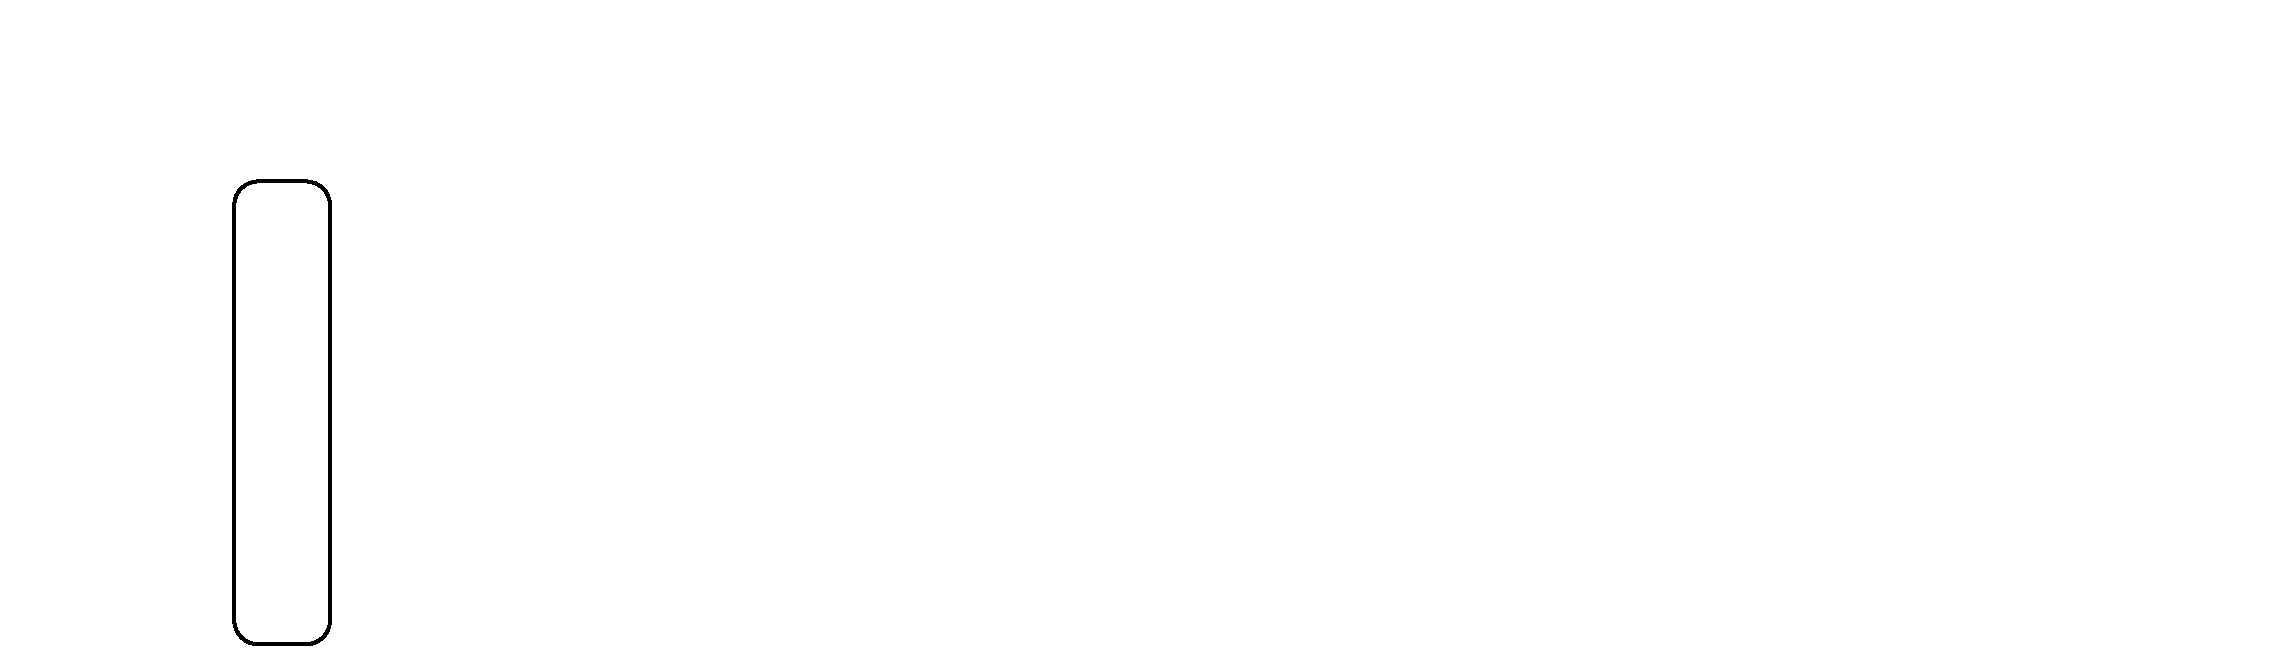
\includegraphics[width=.9\textwidth]{csinet-pro.pdf}
  %     % \medskip
  %     \caption{DualNet-Sph -- CsiNetPro architecture with Spherical Normalization and Bidirectional Reciprocity.}
  %     \label{fig:dualnet-sph-arch}
  %   \end{figure}
  %   \blfootnote{\bibentry{ref:dualnet}}
  % \end{frame}
  % }


  % dualnet results
  % \nofoot{
  % \begin{frame}{Spherical Normalization: Results}
  %   \begin{figure}[!hbtp] \centering 
  %   \subfigure[Indoor] {\label{fignmse:a} 
  %   \includegraphics[width=0.46\textwidth]{images/nmse_indoor.eps}
  %   } 
  %   \subfigure[Outdoor] { \label{fignmse:b} 
  %   \includegraphics[width=0.46\textwidth]{images/nmse_outdoor.eps} 
  %   } 
  %   \caption{NMSE (lower is better) comparison in different compression ratios for downlink-based CSI feedback.\cite{ref:liu2020sphnet}} 
  %   \label{fignmse} \vspace*{-2mm}
  %   \end{figure}
  %   \blfootnote{\bibentry{ref:liu2020sphnet}}
  % \end{frame}
  % }

  % dualnet
  % \nofoot{
  % % 2x2 matrix denoting different test configurations
  % \begin{frame}{Experimental Setup: Models}
  %   \begin{figure}[!hbtp] \centering 
  %     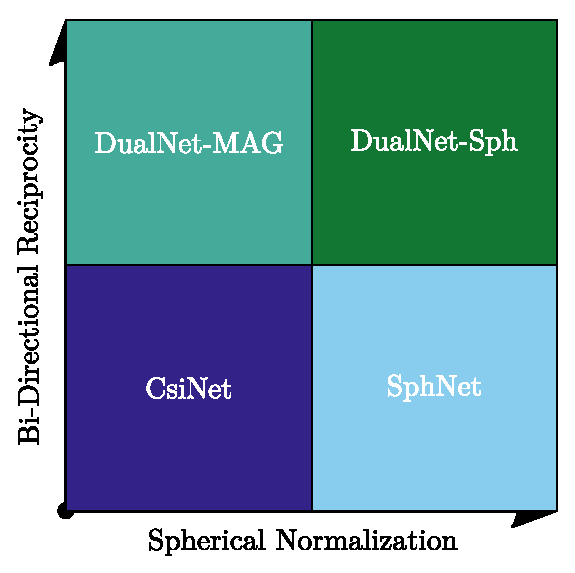
\includegraphics[width=0.47\textwidth]{00-experiment-grid.eps}
  %     \caption{Illustration of techniques used in different models.} 
  %     \label{fig:grid} \vspace*{-2mm}
  %   \end{figure}
  %   \blfootnote{\bibentry{ref:liu2020sphnet}}
  % \end{frame}
  % }

  % csinet-pro/sphnet grid
  \nofoot{
  % 2x2 matrix denoting different test configurations
  \begin{frame}{Experimental Setup: Models}
    \begin{figure}[!hbtp] \centering 
      \fontsize{8pt}{10pt}
      \def\svgwidth{0.47\columnwidth}
      \input{../images/00-experiment-grid-sph.pdf_tex}
      \caption{Illustration of techniques used in different models.} 
      \label{fig:grid} \vspace*{-2mm}
    \end{figure}
    \blfootnote{\bibentry{ref:liu2020sphnet}}
  \end{frame}
  }

  % \begin{frame}{Experimental Setup: Parameters}
  %   Two MIMO scenarios using COST 2100 model with 32 antennas at gNB and single UE (single antenna), 1024 subcarriers.
  %   \begin{enumerate}
  %       \item \textbf{Indoor} environment using 5.3GHz, 0.1 m/s UE mobility, square area of length $20$m
  %       \item \textbf{Outdoor} environment using 300MHz, 1 m/s UE mobility, square area of length $400$m
  %   \end{enumerate}
  %   \textbf{Dataset}: $10^5$ channel samples -- $70\% / 30\% $ training/test split. % vary compression ratio from $\frac{1}{4}$ to $\frac{1}{16}$

  %   \textbf{Hyperparameters}: Adam optimizer with learning rate $10^{-3},$ batch size $200,$ $1000$ epochs, MSE loss
  % \end{frame}

  \nofoot{
  \begin{frame}{Experimental Setup: Parameters}
    \begin{table}[htb]
      \begin{center}
        \caption{Parameters for COST2100 model in this work.}
        \label{tab:cost2100-params} 
        \begin{tabular}{|l|c|c|}
          \hline 
          \textbf{Environment}      & \textbf{Indoor}  & \textbf{Outdoor} \\ \hline
          Num. gNB Antennas ($N_b$) & \multicolumn{2}{c|}{32} \\ \hline
          Num. Subcarriers ($N_f$)  & \multicolumn{2}{c|}{1024} \\ \hline
          Truncation Value ($R_d$)  & \multicolumn{2}{c|}{32} \\ \hline
          Carrier Frequency         & 5.3 GHz            & 300 MHz \\ \hline
          UE Mobility               & 0.001 m/s        & 1 m/s \\ \hline
          UE Starting Position      & $20 \times 20$ m & $400 \times 400$ m \\ \hline
          Num. Channel Samples ($N$)& \multicolumn{2}{c|}{$10^5$} \\ \hline
          Training/Validation Split & \multicolumn{2}{c|}{70\%/30\%} \\ \hline
          Feedback interval         & \multicolumn{2}{c|}{$40$ ms} \\ \hline
        \end{tabular}
      \end{center}
    \end{table}
    \blfootnote{\bibentry{ref:liu2012cost2100}}
  \end{frame}
  }

  % dualnet
  % \nofoot{
  % \begin{frame}{Experimental Results}
  %   \begin{figure}[!hbtp] \centering 
  %     \subfigure[Indoor] {\label{fignmse_mag:a} 
  %     % \includegraphics[width=0.46\textwidth]{images/nmse_indoor_mag.eps}
  %     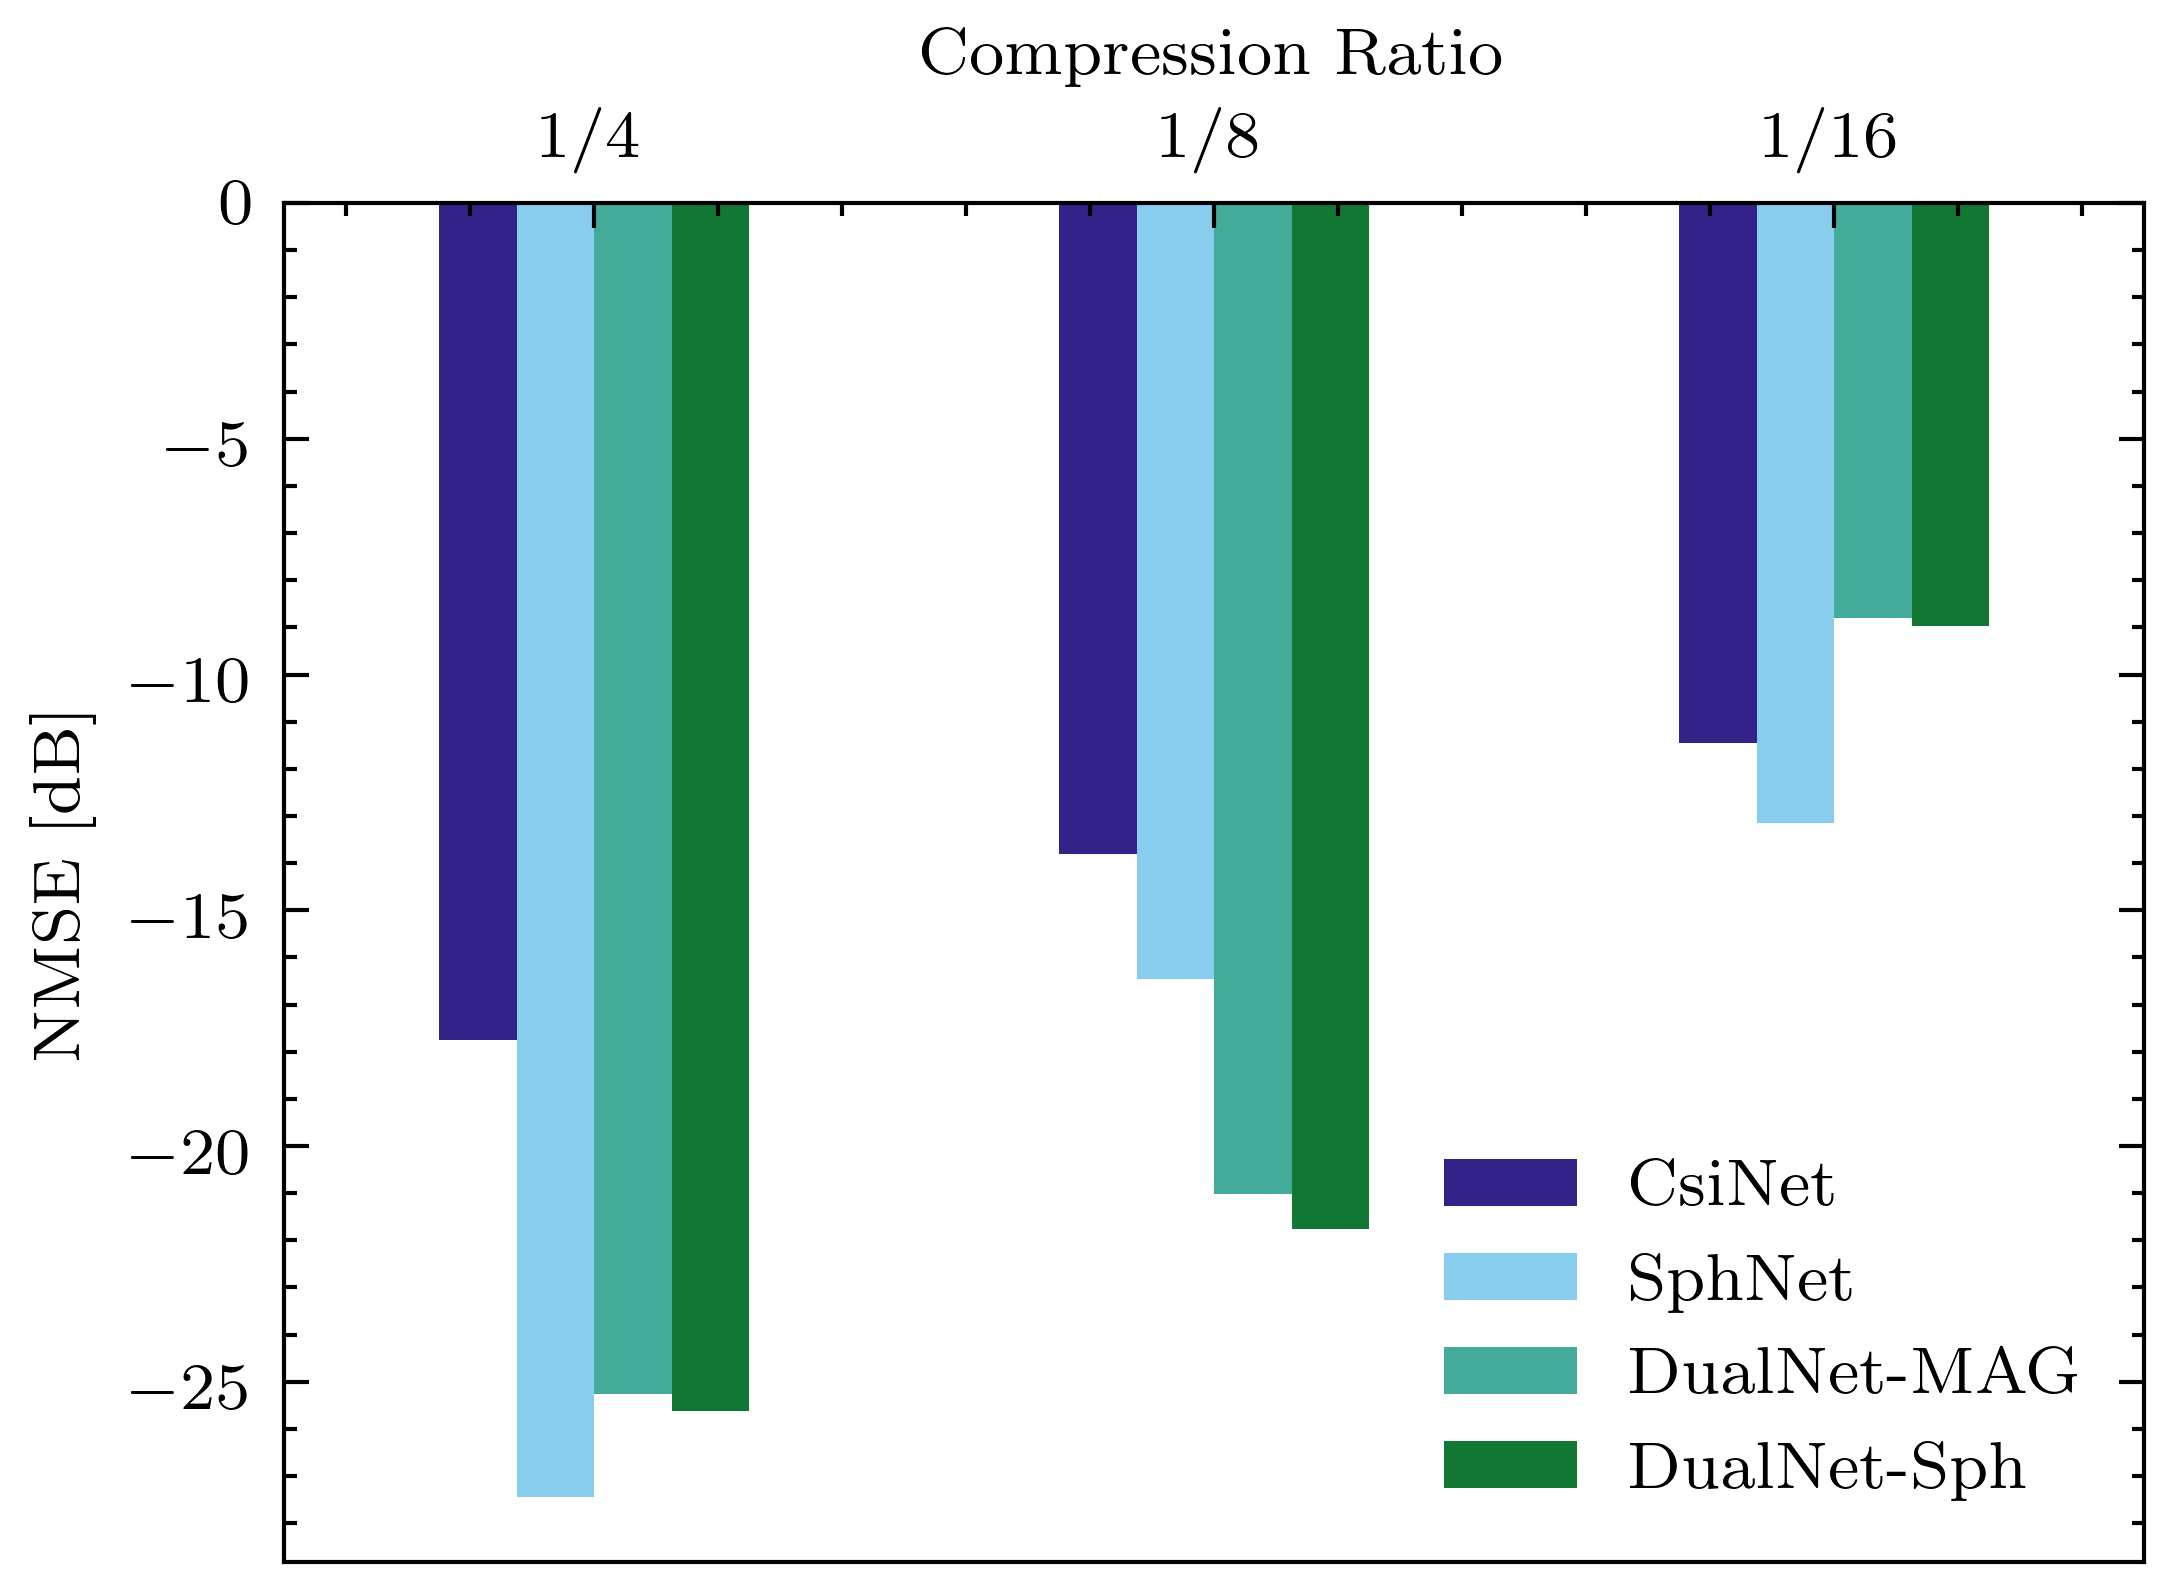
\includegraphics[width=0.47\textwidth]{indoor_res.png}
  %     } 
  %     \subfigure[Outdoor] { \label{fignmse_mag:b} 
  %     % \includegraphics[width=0.46\textwidth]{images/nmse_outdoor_mag.eps} 
  %     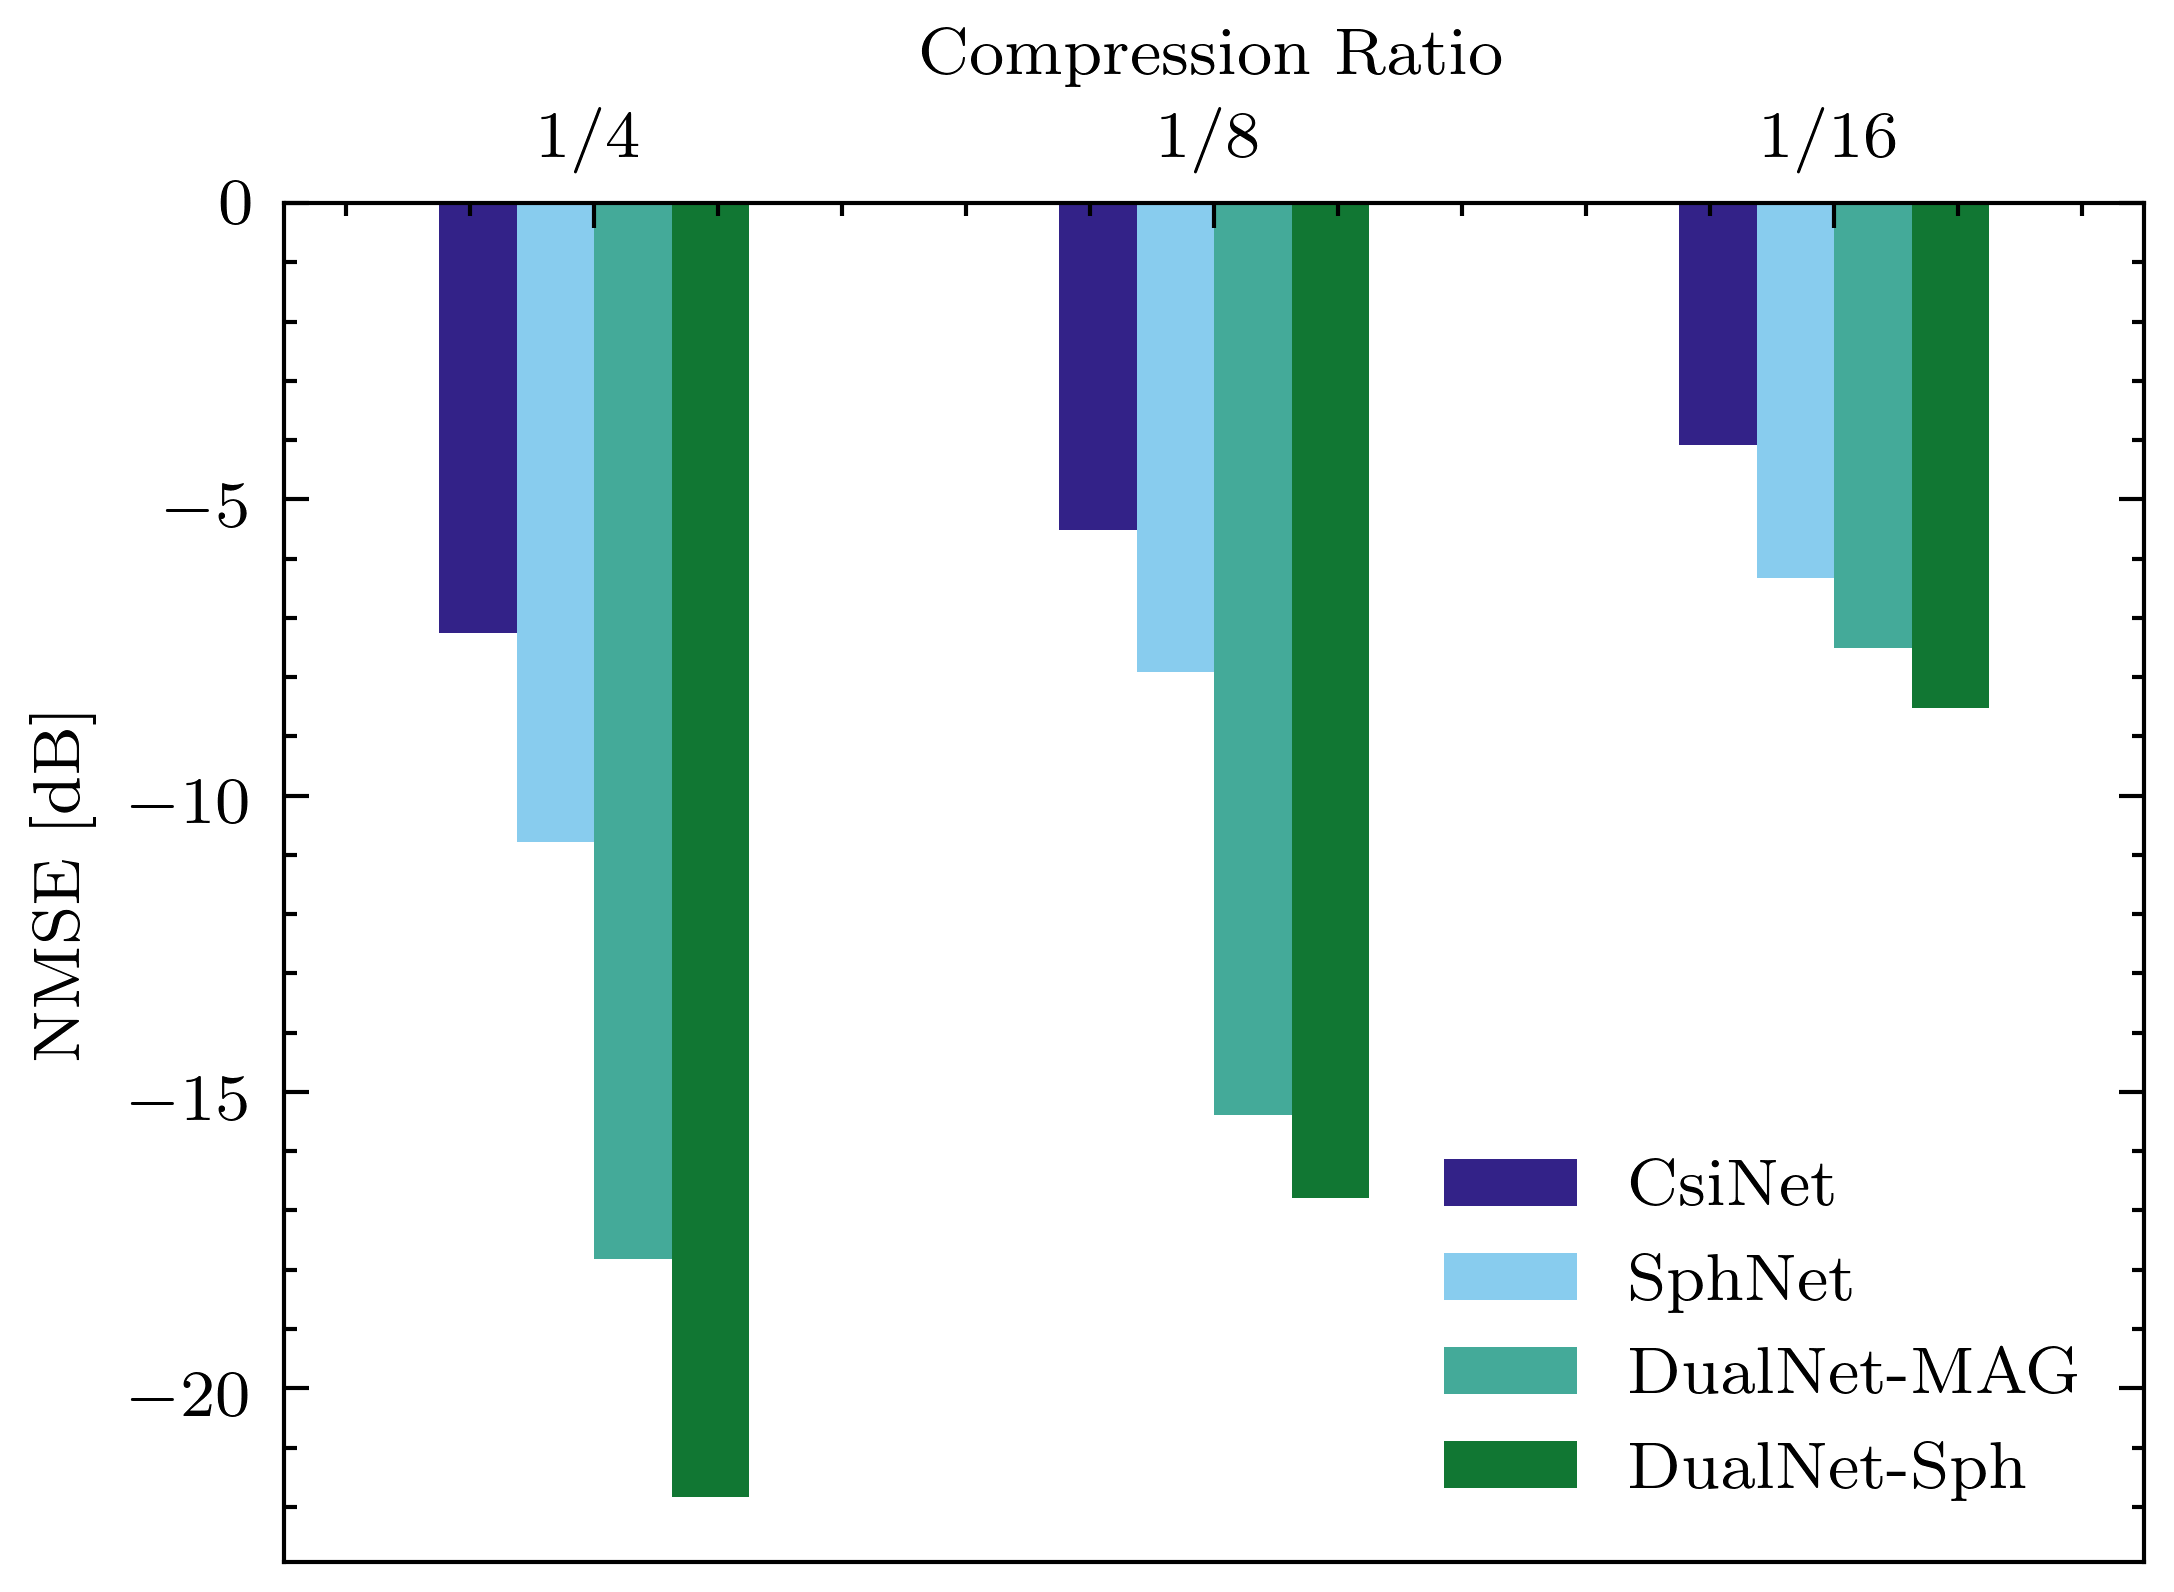
\includegraphics[width=0.47\textwidth]{outdoor_res.png}
  %     } 
  %     \caption{NMSE (lower is better) comparison of bidirectional reciprocity and spherical normalization against CsiNet for increasing compression ratio \cite{ref:liu2020sphnet}} 
  %     \label{fignmse_mag} \vspace*{-2mm}
  %   \end{figure}
  %   \blfootnote{\bibentry{ref:liu2020sphnet}}
  % \end{frame}
  % }

  % csinet-pro, sphnet
  \nofoot{
  \begin{frame}{Experimental Results}
    \begin{figure}[!hbtp] \centering 
      \subfigure[Indoor]{
        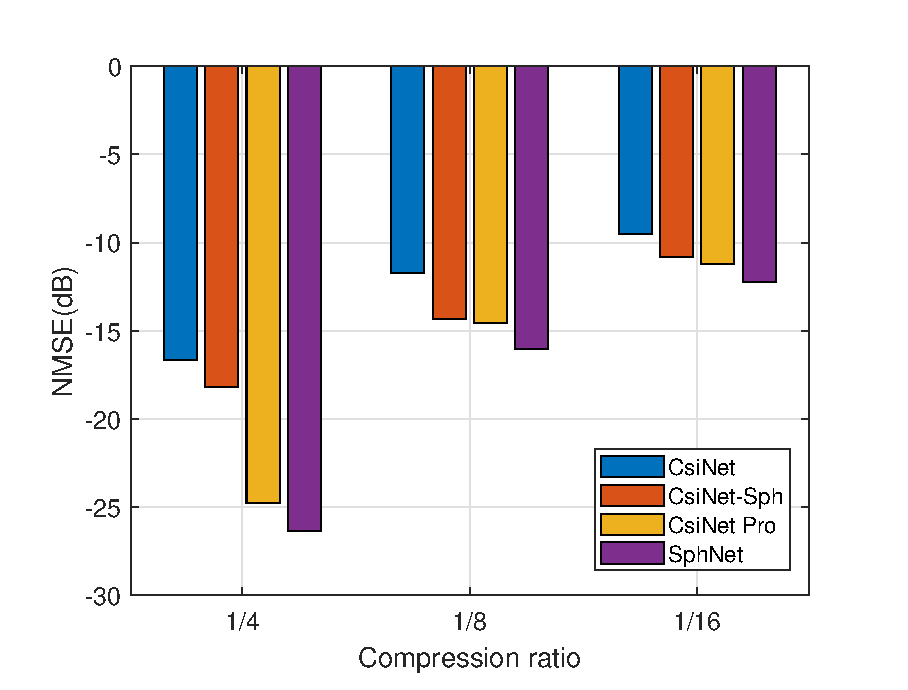
\includegraphics[width=.45\textwidth]{nmse_slot1_indoor.eps}
        \label{fig:slot1_indoor} 
      }
      \subfigure[Outdoor]{
        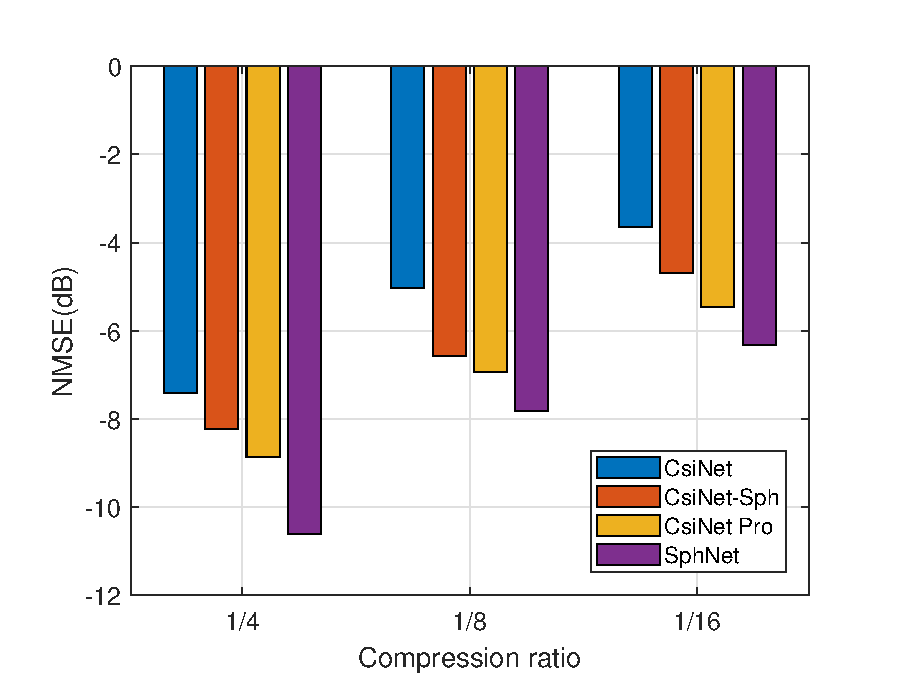
\includegraphics[width=.45\textwidth]{nmse_slot1_outdoor.eps}
        \label{fig:slot1_outdoor} 
      }
      \caption{Ablation study for CsiNet-Pro and spherical normalization \cite{ref:liu2020sphnet} (lower NMSE is better).}
      \label{fig:nmse_slot1} 
    \end{figure}
    \blfootnote{\bibentry{ref:liu2020sphnet}}
  \end{frame}
  }

\section{Completed Work \#2: MarkovNet}
  % MarkovNet section frame 
  \begin{frame}[plain]
    \vfill
    \centering
    \begin{beamercolorbox}[sep=8pt,center,shadow=true,rounded=true]{MarkovNet}
      \usebeamerfont{title}\insertsectionhead\par%
      \color{davisblue}\noindent\rule{10cm}{1pt} \\
      \footnotesize{A deep differential autoencoder for efficient temporal learning.}
      % \LARGE{\faFileTextO}
    \end{beamercolorbox}
    \vfill
  \end{frame}

  % DONE: add figure demonstrating temporal CSI? snapshots of t_1, t_2, ..., t_3
  \begin{frame}{Temporal Correlation}
    \begin{figure}[htb] \centering 
      % 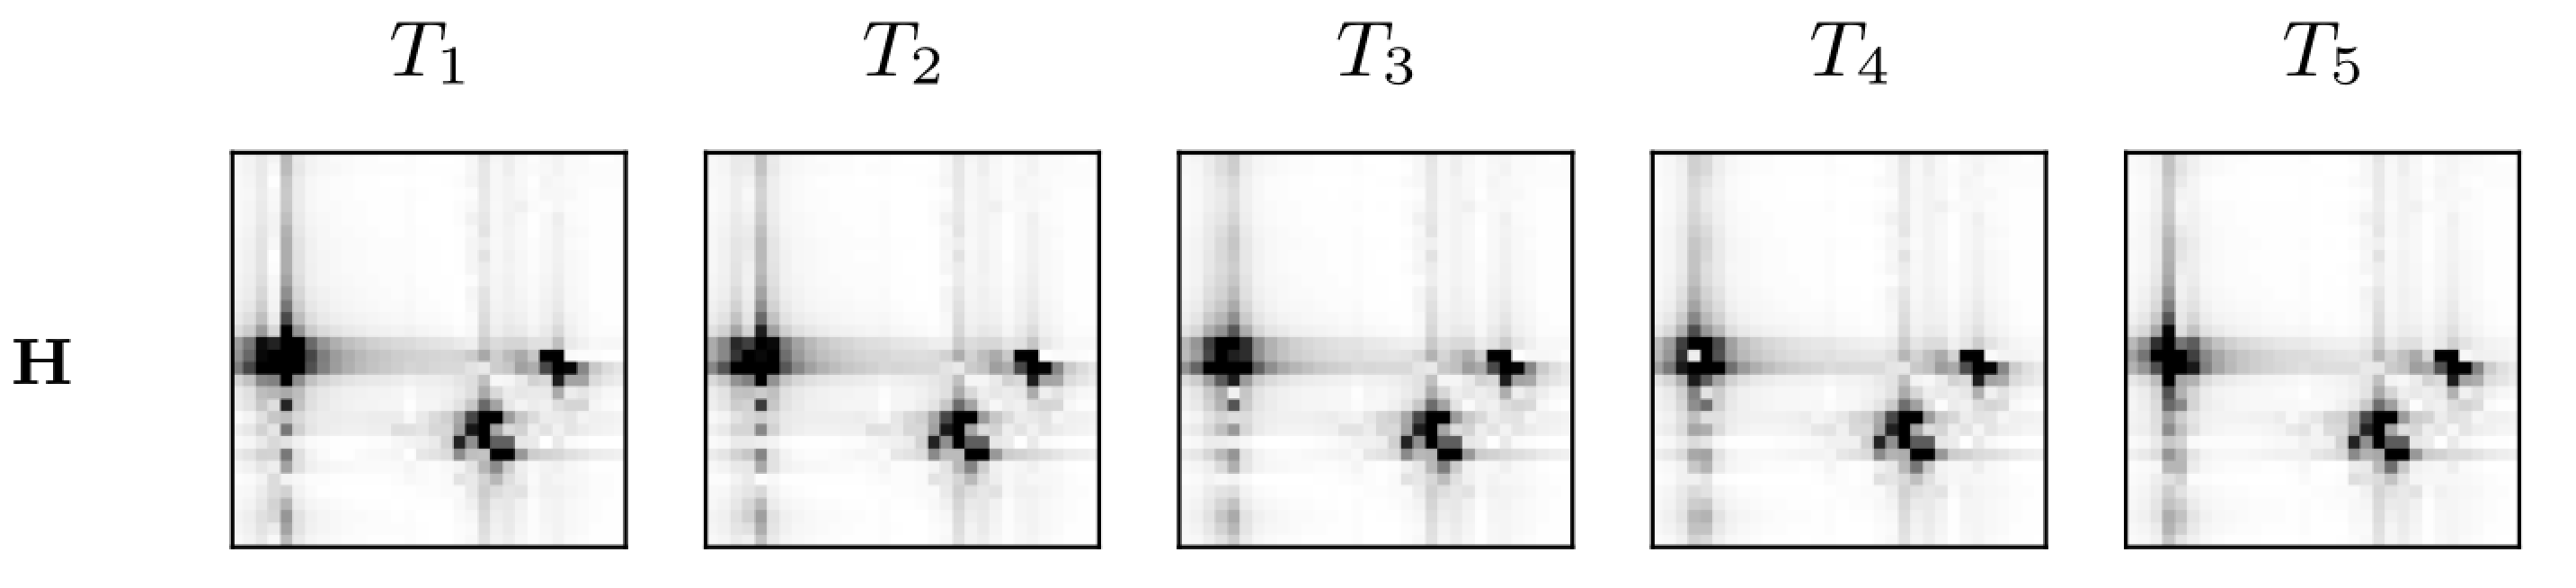
\includegraphics[width=0.9\linewidth]{batch0_csi_gt.png}
    {
      \fontsize{10pt}{12pt}
      \def\svgwidth{1.0\columnwidth}
      \input{../images/batch0_csi_gt.pdf_tex}
    }
      \caption{Ground truth CSI ($\mathbf H$) for five timeslots ($T_1$ through $T_5$) on one outdoor sample from the validation set.} 
      \label{fig:csi_img_gt} 
    \end{figure}
  \end{frame}
  % TODO: change to LaTeX-annotated 

  % entropy/cond entropy
  % \begin{frame}{Temporal Correlation}
  %   CSI estimation benefit from temporal information.
  %   \begin{figure}[!hbtp] \centering 
  %     \subfigure[Indoor] {\label{fig:entropy_in} 
  %     % \includegraphics[width=0.46\textwidth]{images/nmse_indoor_mag.eps}
  %     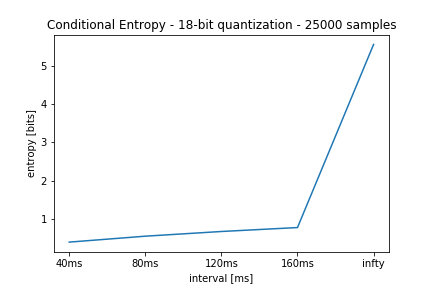
\includegraphics[width=0.47\textwidth]{indoor_entropy.png}
  %     } 
  %     \subfigure[Outdoor] { \label{fig:entropy_out} 
  %     % \includegraphics[width=0.46\textwidth]{images/nmse_outdoor_mag.eps} 
  %     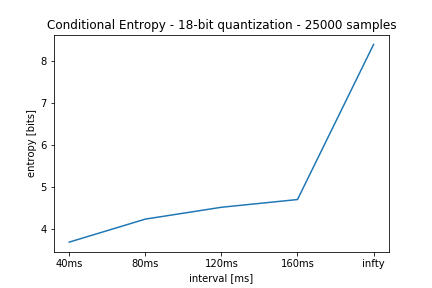
\includegraphics[width=0.47\textwidth]{outdoor_entropy.png}
  %     } 
  %     \caption{Conditional entropy between CSI matrices for different feedback intervals. Data generated with COST2100 model.} 
  %     \label{fig:entropy} \vspace*{-2mm}
  %   \end{figure}
  % \end{frame}

  \nofoot{
  \begin{frame}{Recurrent Neural Networks for Temporal Correlation}
    \footnotesize{
    Recurrent neural networks (RNNs) contain trainable long short-term memory (LSTM) cells which learn temporal relationships. 
    \begin{figure}[htb] \centering 
      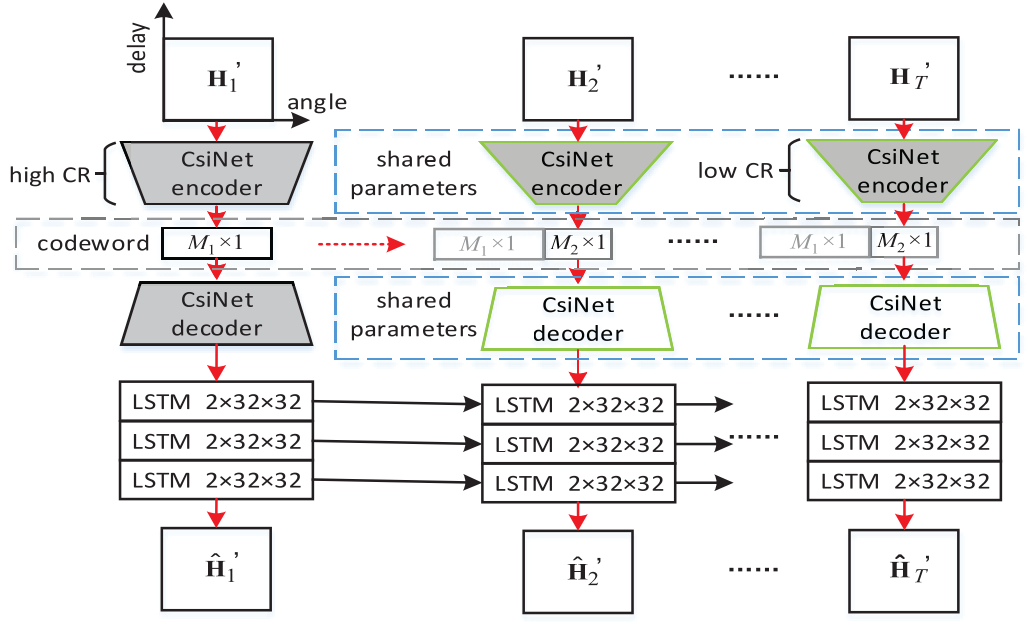
\includegraphics[width=0.6\linewidth]{csinet-lstm.png}
      \caption{CsiNet-LSTM network architecture \cite{ref:Wang2019CsiNetLSTM}.} 
      \label{fig:csinet-lstm} 
    \end{figure}
    }
    \blfootnote{\bibentry{ref:Wang2019CsiNetLSTM}}
  \end{frame}
  }

  \nofoot{
  \begin{frame}{CsiNet-LSTM Performance}
    \begin{columns}
      \begin{column}{0.4\textwidth}
        \footnotesize{
        LSTMs improve NMSE at smaller compression ratios.
        }
      \end{column}
      \begin{column}{0.6\textwidth}  %%<--- here
        \fignocap{1.0}{csinet-lstm-results.PNG}
      \end{column}
    \end{columns}
    \blfootnote{\bibentry{ref:Wang2019CsiNetLSTM}}
  \end{frame}
  }

  \nofoot{
  \begin{frame}{CsiNet-LSTM Complexity}
    % \footnotesize{
    \textbf{Problem:} Number of parameters/FLOPs for RNNs is large.
    \begin{table}[htb]
      % \renewcommand{\arraystretch}{1.5}
      \begin{center}
        \caption{Model size/computational complexity per timeslot for CsiNet-LSTM and CsiNet. M: million.}
        \label{tab:comp-complex-lstm-only} 
        \begin{tabular}{|c|c|c|c|c|}
        \hline
                    & \multicolumn{2}{c|}{\textbf{Parameters}} & \multicolumn{2}{c|}{\textbf{FLOPs}} \\ \hline 
        \textbf{CR} & \textbf{CsiNet-LSTM} & \textbf{CsiNet} & \textbf{CsiNet-LSTM} & \textbf{CsiNet} \\ \hline
        $1/4$       & 132.7 M        & 2.1 M        & 412.9 M        & 7.8 M              \\ \hline
        $1/8$       & 123.2 M        & 1.1 M        & 410.8 M        & 5.7 M              \\ \hline
        $1/16$      & 118.5 M        & 0.5 M        & 409.8 M        & 4.7 M              \\ \hline
        $1/32$      & 116.1 M        & 0.3 M        & 409.2 M        & 4.1 M              \\ \hline
        $1/64$      & 115.0 M        & 0.1 M        & 409.0 M        & 3.9 M              \\ \hline
        \end{tabular}
      \end{center}
    \end{table}
    % \blfootnote{\bibentry{ref:Wang2019CsiNetLSTM}}
  \end{frame}
  % }
  }

  % \subsection{Differential Encoding}
  \nofoot{
  \begin{frame}{Markov Assumption}
    % Instead of learning a temporal dependency
    % across multiple timeslots,
    % We proposed a simplified \textbf{one-step differential encoder}.

    For short enough feedback interval,
    % between $t$ and $t-1$, 
    % CSI data are stationary, i.e. 
    CSI data form a Markov chain,
    \begin{align*} 
      \mathbf H_t &= \gamma\mathbf H_{t-1} + \mathbf V_t,
    \end{align*}
    with $\gamma \in \mathbb R^+$ and i.i.d $\mathbf
    V_t \sim \mathcal{CN}(\mathbf 0,\Sigma_V)$.
    % $\mathbb E\left[\mathbf V_t\right] = \mathbf 0$.
    \footnotesize{
    \blfootnote{\bibentry{ref:Liu2020MarkovNet} (\textdagger \; equal contribution)} 
    }
  \end{frame}
  }

  \begin{frame}{Scalar One-step Estimation}
    The ordinary least-squares solution, $\gamma$, is given as
    \begin{align*}
      \gamma &= \frac{\text{Trace}(\mathbb E\left[\mathbf H_{t-1}^H\mathbf H_{t}\right])}{\mathbb E\Arrowvert\mathbf H_t^H \mathbf H_t\Arrowvert^2}.
    \end{align*}
    \pause
    Utilize estimator, $\hat \gamma$, based on the sample statistics, % of the CSI matrices,
    \begin{align*}
      \hat \gamma &= \frac{\sum_{i=1}^N\text{Trace}(\left[\mathbf H_{t-1}^H(i)\mathbf H_{t}(i)\right])}{\sum_{i=1}^N\Arrowvert\mathbf H_t^H(i) \mathbf H_t(i)\Arrowvert^2},
    \end{align*}
    for training set of size $N$.
  \end{frame}

  \begin{frame}{Differential Encoding}
    Using $\hat\gamma$, train encoder on estimation error as
    \begin{align*}
      \mathbf E_{t} &= \mathbf H_t - \hat \gamma \hat {\mathbf H}_{t-1} \\
      \mathbf z_t &= f_{e,t} (\mathbf E_t).
    \end{align*}
    Jointly train a decoder,
    \begin{align*}
      \hat{\mathbf E}_t &= f_{d,t}(\mathbf z_t) \\
      \hat{\mathbf H}_t &= \hat{\mathbf E}_t + \hat\gamma\hat{\mathbf H}_{t-1}.
    \end{align*}
  \end{frame}

  \begin{frame}{MarkovNet: Deep Differential Encoding}
    \begin{figure}[!hbtp]
    \centering
    {
      \fontsize{4pt}{6pt}
      \def\svgwidth{0.8\columnwidth}
      \input{../images/markovnet_schematic.pdf_tex}
    }
    \caption{MarkovNet architecture. Networks at $t \geq 2$ predict estimation error, $\hat{\mathbf E}_t$.}
    \label{fig:markovnet_schema}
    \end{figure}
  \end{frame}

  \begin{frame}{MarkovNet Results -- NMSE Performance}
    \begin{figure}[!hbtp] \centering 
      \subfigure[Indoor] {\label{fig:diffnet_indoor} 
      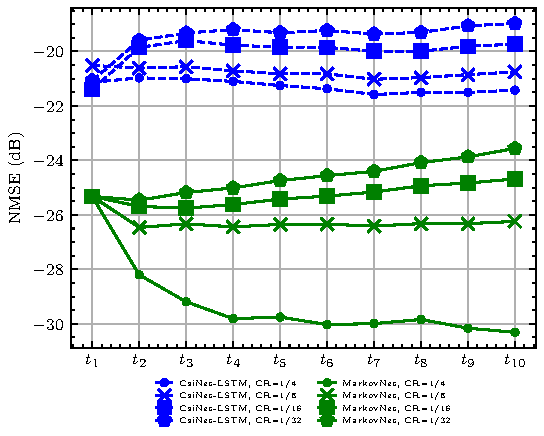
\includegraphics[width=0.46\textwidth]{MarkovNet_truncated_Indoor_10slots.pdf}
      } 
      \subfigure[Outdoor] { \label{fig:diffnet_outdoor} 
      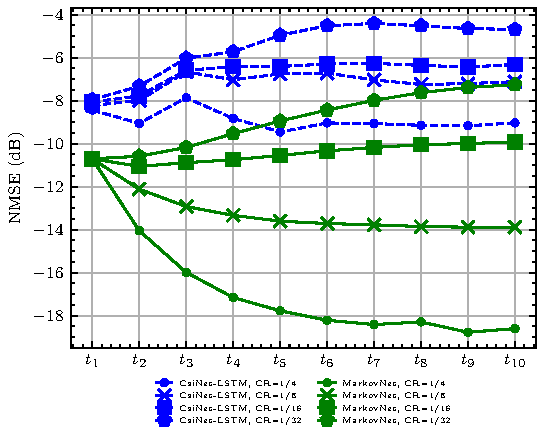
\includegraphics[width=0.46\textwidth]{MarkovNet_truncated_Outdoor_10slots.pdf} 
      } 
      \vspace*{-3mm}

      \caption{$\text{NMSE}$ (lower is better) comparison of MarkovNet and CsiNet-LSTM 
      at multiple CRs.} 
      \label{fig:diffnet_result} \vspace*{-2mm}
    \end{figure}  
  \end{frame}

  \begin{frame}{MarkovNet Results -- CSI Images}
    \begin{figure}[htb] \centering 
      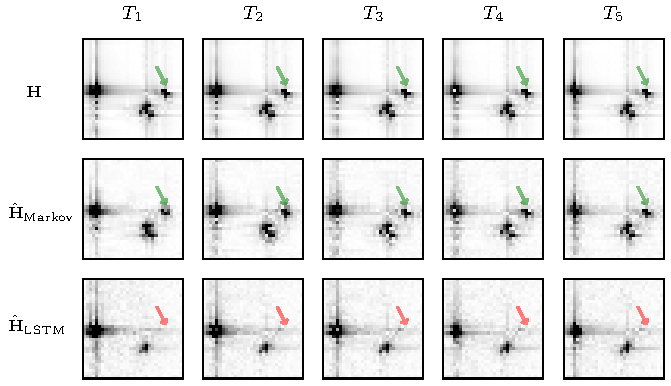
\includegraphics[width=0.9\linewidth]{batch0_csi_compare_cr512_annot.pdf}
      \caption{Ground truth ($\mathbf H$), MarkovNet estimates ($\hat{\mathbf H}_{\text{Markov}}$), and CsiNet-LSTM estimates ($\hat{\mathbf H}_{\text{LSTM}}$) on from outdoor test set ($\text{CR}=\frac 14$).} 
      \label{fig:csi_img_compare} 
    \end{figure}
  \end{frame}

  \nofoot{
  \begin{frame}{MarkovNet: Computational Complexity}
    \footnotesize{
    \begin{table}[htb]
      \renewcommand{\arraystretch}{1}
      \begin{center}
      % \caption{Table II: Model size \& computational complexity comparison. M: million, K: thousand.}
      \caption{Model size/computational complexity of tested temporal networks (CsiNet-LSTM, MarkovNet) and comparable non-temporal network (CsiNet). M: million.}
      \label{tab:comp-complex} 
      % \resizebox{\linewidth}{15mm}
      {
      \begin{tabular}{|l|c|c|c|c|}
      \hline
                                  & \multicolumn{3}{c|}{\textbf{Parameters}}                                                                                 \\ \hline
                                  & \textbf{CsiNet-LSTM} & \textbf{MarkovNet} & \textbf{CsiNet} \\ \hline
      \textbf{CR=$1/4$}  & 132.7 M              & 2.1 M              & 2.1 M          \\ \hline
      \textbf{CR=$1/8$}  & 123.2 M              & 1.1 M              & 1.1 M          \\ \hline
      \textbf{CR=$1/16$} & 118.5 M              & 0.5 M              & 0.5 M          \\ \hline
      \textbf{CR=$1/32$} & 116.1 M              & 0.3 M              & 0.3 M          \\ \hline
      \textbf{CR=$1/64$} & 115.0 M              & 0.1 M              & 0.1 M          \\ \hline
                                  & \multicolumn{3}{c|}{\textbf{FLOPs}}                                                                                      \\ \hline
                                  & \textbf{CsiNet-LSTM} & \textbf{MarkovNet} & \textbf{CsiNet} \\ \hline
      \textbf{CR=$1/4$}  & 412.9 M              & 44.5 M             & 7.8 M          \\ \hline
      \textbf{CR=$1/8$}  & 410.8 M              & 42.4 M             & 5.7 M          \\ \hline
      \textbf{CR=$1/16$} & 409.8 M              & 41.3 M             & 4.7 M          \\ \hline
      \textbf{CR=$1/32$} & 409.2 M              & 40.8 M             & 4.1 M          \\ \hline
      \textbf{CR=$1/64$} & 409.0 M              & 40.5 M             & 3.9 M          \\ \hline
      \end{tabular}
      }
      \end{center}
    \end{table} 
    }
  \end{frame}
  }

\section{Completed Work \#3: Pilots-to-delay Estimator (P2DE) and Heterogeneous Differential Encoding}

  % Background section frame 
  \begin{frame}[plain]
    \vfill
    \centering
    \begin{beamercolorbox}[sep=8pt,center,shadow=true,rounded=true]{P2DE/Heterogeneous MarkovNet}
      \usebeamerfont{title}\insertsectionhead\par%
      \color{davisblue}\noindent\rule{10cm}{1pt} \\
      \footnotesize{Acquiring delay domain CSI under practical pilot placement. Improving differential encoding.} 
      % \LARGE{\faFileTextO}
    \end{beamercolorbox}
    \vfill
  \end{frame}

  \nofoot{
  \begin{frame}{Delay Domain CSI}
      \textbf{Recall:} Works in DL-based CSI compression have used delay domain.
      \fignocap{0.9}{csinet-fig-paper.PNG}
      \blfootnote{\bibentry{ref:csinet}}
  \end{frame}
  }

  \begin{frame}{Frequency Domain Pilots}
    \textbf{Problem:} CSI at UE is based on sparse pilot estimates.
    \begin{figure}[!hbtp]
    \centering
    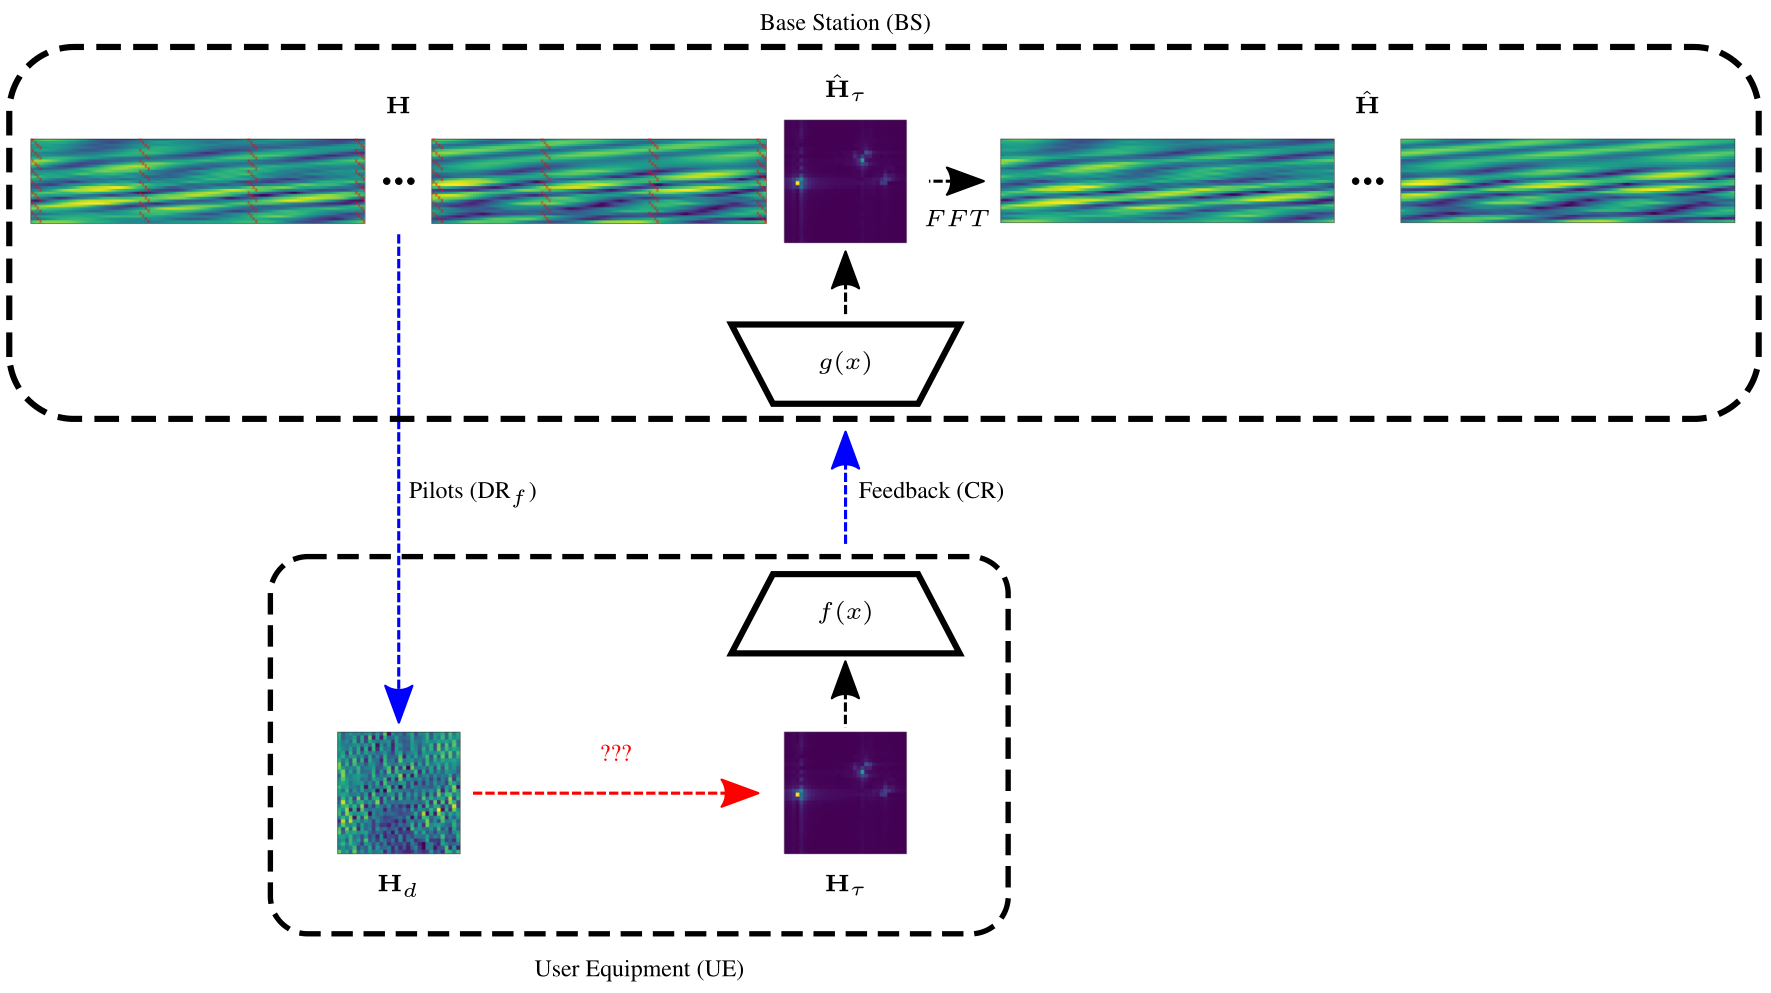
\includegraphics[width=\linewidth]{../images/00_downlink_no_p2d_feedback_horiz_diag.png}
    \label{fig:no_p2d}
    \end{figure}
  \end{frame}

  \begin{frame}{Downsampled Frequency Domain CSI}
    \begin{itemize}
      \item Denote $\boldeta_i \in \mathbb{C}^{N_f}$ as the $i$-th row of the spatial-frequency matrix $\mathbf{H}$
      \item Denote the downsampled version of $\boldeta_i$ as $\boldeta_{d,i} \in \mathbb{C}^{M_f}$ where $M_f << N_f$
      \item The spatial-frequency CSI, $\mathbf{H}$, and its downsampled counterpart, $\mathbf{H}_d$, can be written as,
      \begin{equation}
        \mathbf{H} = \begin{bmatrix} \boldeta_1 \\ \boldeta_2 \\ \vdots \\ \boldeta_{N_b} \\\end{bmatrix}\in\mathbb{C}^{N_b \times N_f}, \; \mathbf{H}_d = \begin{bmatrix} \boldeta_{d,1} \\ \boldeta_{d,2} \\ \vdots \\ \boldeta_{d,N_b} \\\end{bmatrix}\in\mathbb{C}^{N_b \times M_f}.
      \end{equation}
    \end{itemize}
  \end{frame}

  \begin{frame}{Downsampled Frequency Domain CSI}
    $\boldeta_{d,i}$ is related to $\boldeta_i$ by the downsampling matrix for the $i$-th antenna port, $\mathbf{P}_i$, as
    \begin{equation}
      \boldeta_{d,i} = \boldeta_i \mathbf{P}_i \; \forall \; i \in [1, \dots, N_b],
    \end{equation}
    where $\mathbf{P}_i$ (matrix of one-hot vectors) is chosen to conform with 3GPP-defined pilot allocation.
  \end{frame}

  \begin{frame}{Pilots to Delay Domain}
    \begin{figure}[!hbtp]
    \centering
    {
      \fontsize{6pt}{6pt}
      \def\svgwidth{0.8\columnwidth}
      \input{../images/pilot_downsampling_process.pdf_tex}
    }
    % \caption{MarkovNet architecture. Networks at $t \geq 2$ predict estimation error, $\hat{\mathbf E}_t$.}
    \label{fig:pilot_downsampling}
    \end{figure}
  \end{frame}

  \begin{frame}{Pilots to Delay Domain}
    Denote the delay-domain CSI vector, $\tilde{\boldeta}_i$, which is defined as
    \begin{equation}
      \tilde{\boldeta}_{i}\mathbf{F} = \boldeta_i, \label{eq:dft}
    \end{equation}
    where $\mathbf{F}$ is the $\mathbf{C}^{N_f \times N_f}$ discrete Fourier transform (DFT) matrix.
  \end{frame}

  \begin{frame}{Pilots to Delay Domain}
    Apply the pilot downsampling matrix $\mathbf{P}_i$ to both sides of (\ref{eq:dft}),
    \begin{align}
      \tilde{\boldeta}_{i}\mathbf{F}\mathbf{P}_i = \boldeta_i\mathbf{P}_i \nonumber \\
      \tilde{\boldeta}_{i}\mathbf{Q}_i = \boldeta_{d,i} \label{eq:qmat}
    \end{align}
    where $\mathbf{Q}_i=\mathbf{F}\mathbf{P}_i\in\mathbb{C}^{N_f\times M_f}$ is the downsampled DFT matrix.
  \end{frame}

  \begin{frame}{Pilots to Delay Domain}
    \begin{itemize}    
      \item \textbf{Recall our goal:} To feed back and compress the truncated delay domain vectors, $\tilde{\boldeta}_{c,i}\in\mathbb{C}^{N_t}$.
      \item Denote the zero-padded vector $\tilde{\boldeta}_{i}$ as
      \begin{align} 
        \tilde{\boldeta}_{i} = \left[\tilde{\boldeta}_{c,i}, \mathbf{0}_{N_f - N_t}\right]. \label{eq:p2d_short}
      \end{align}
      \item Based on $\mathbf{Q}_i$ of (\ref{eq:qmat}), the delay domain is related to the pilots by the pseudoinverse,
      \begin{align}
        \tilde{\boldeta}_{i}\mathbf{Q}_i\mathbf{Q}_i^T &= \boldeta_{d,i}\mathbf{Q}_i^T \nonumber \\
        \tilde{\boldeta}_{i} &= \boldeta_{d,i}\mathbf{Q}_i^T\left(\mathbf{Q}_i\mathbf{Q}_i^T\right)^{-1} \nonumber \\
        &= \boldeta_{d,i}\mathbf{Q}_i^{\#}. \label{eq:p2d}
      \end{align}
    \end{itemize}
  \end{frame}

  \nofoot{
  \begin{frame}{Pilot Pattern Design}
    \footnotesize{
    \begin{itemize}
      \item In 5G subframes, downlink pilots are allocated as \textbf{Demodulation Reference Signals (DM-RS)}.
      \item `Diagonal' pilot pattern in spatial/frequency domain allows faster pilot CSI acquisition (inversely proportional to diagonal size, $D$)
    \end{itemize}
    \begin{figure}[!hbtp]
      \centering
      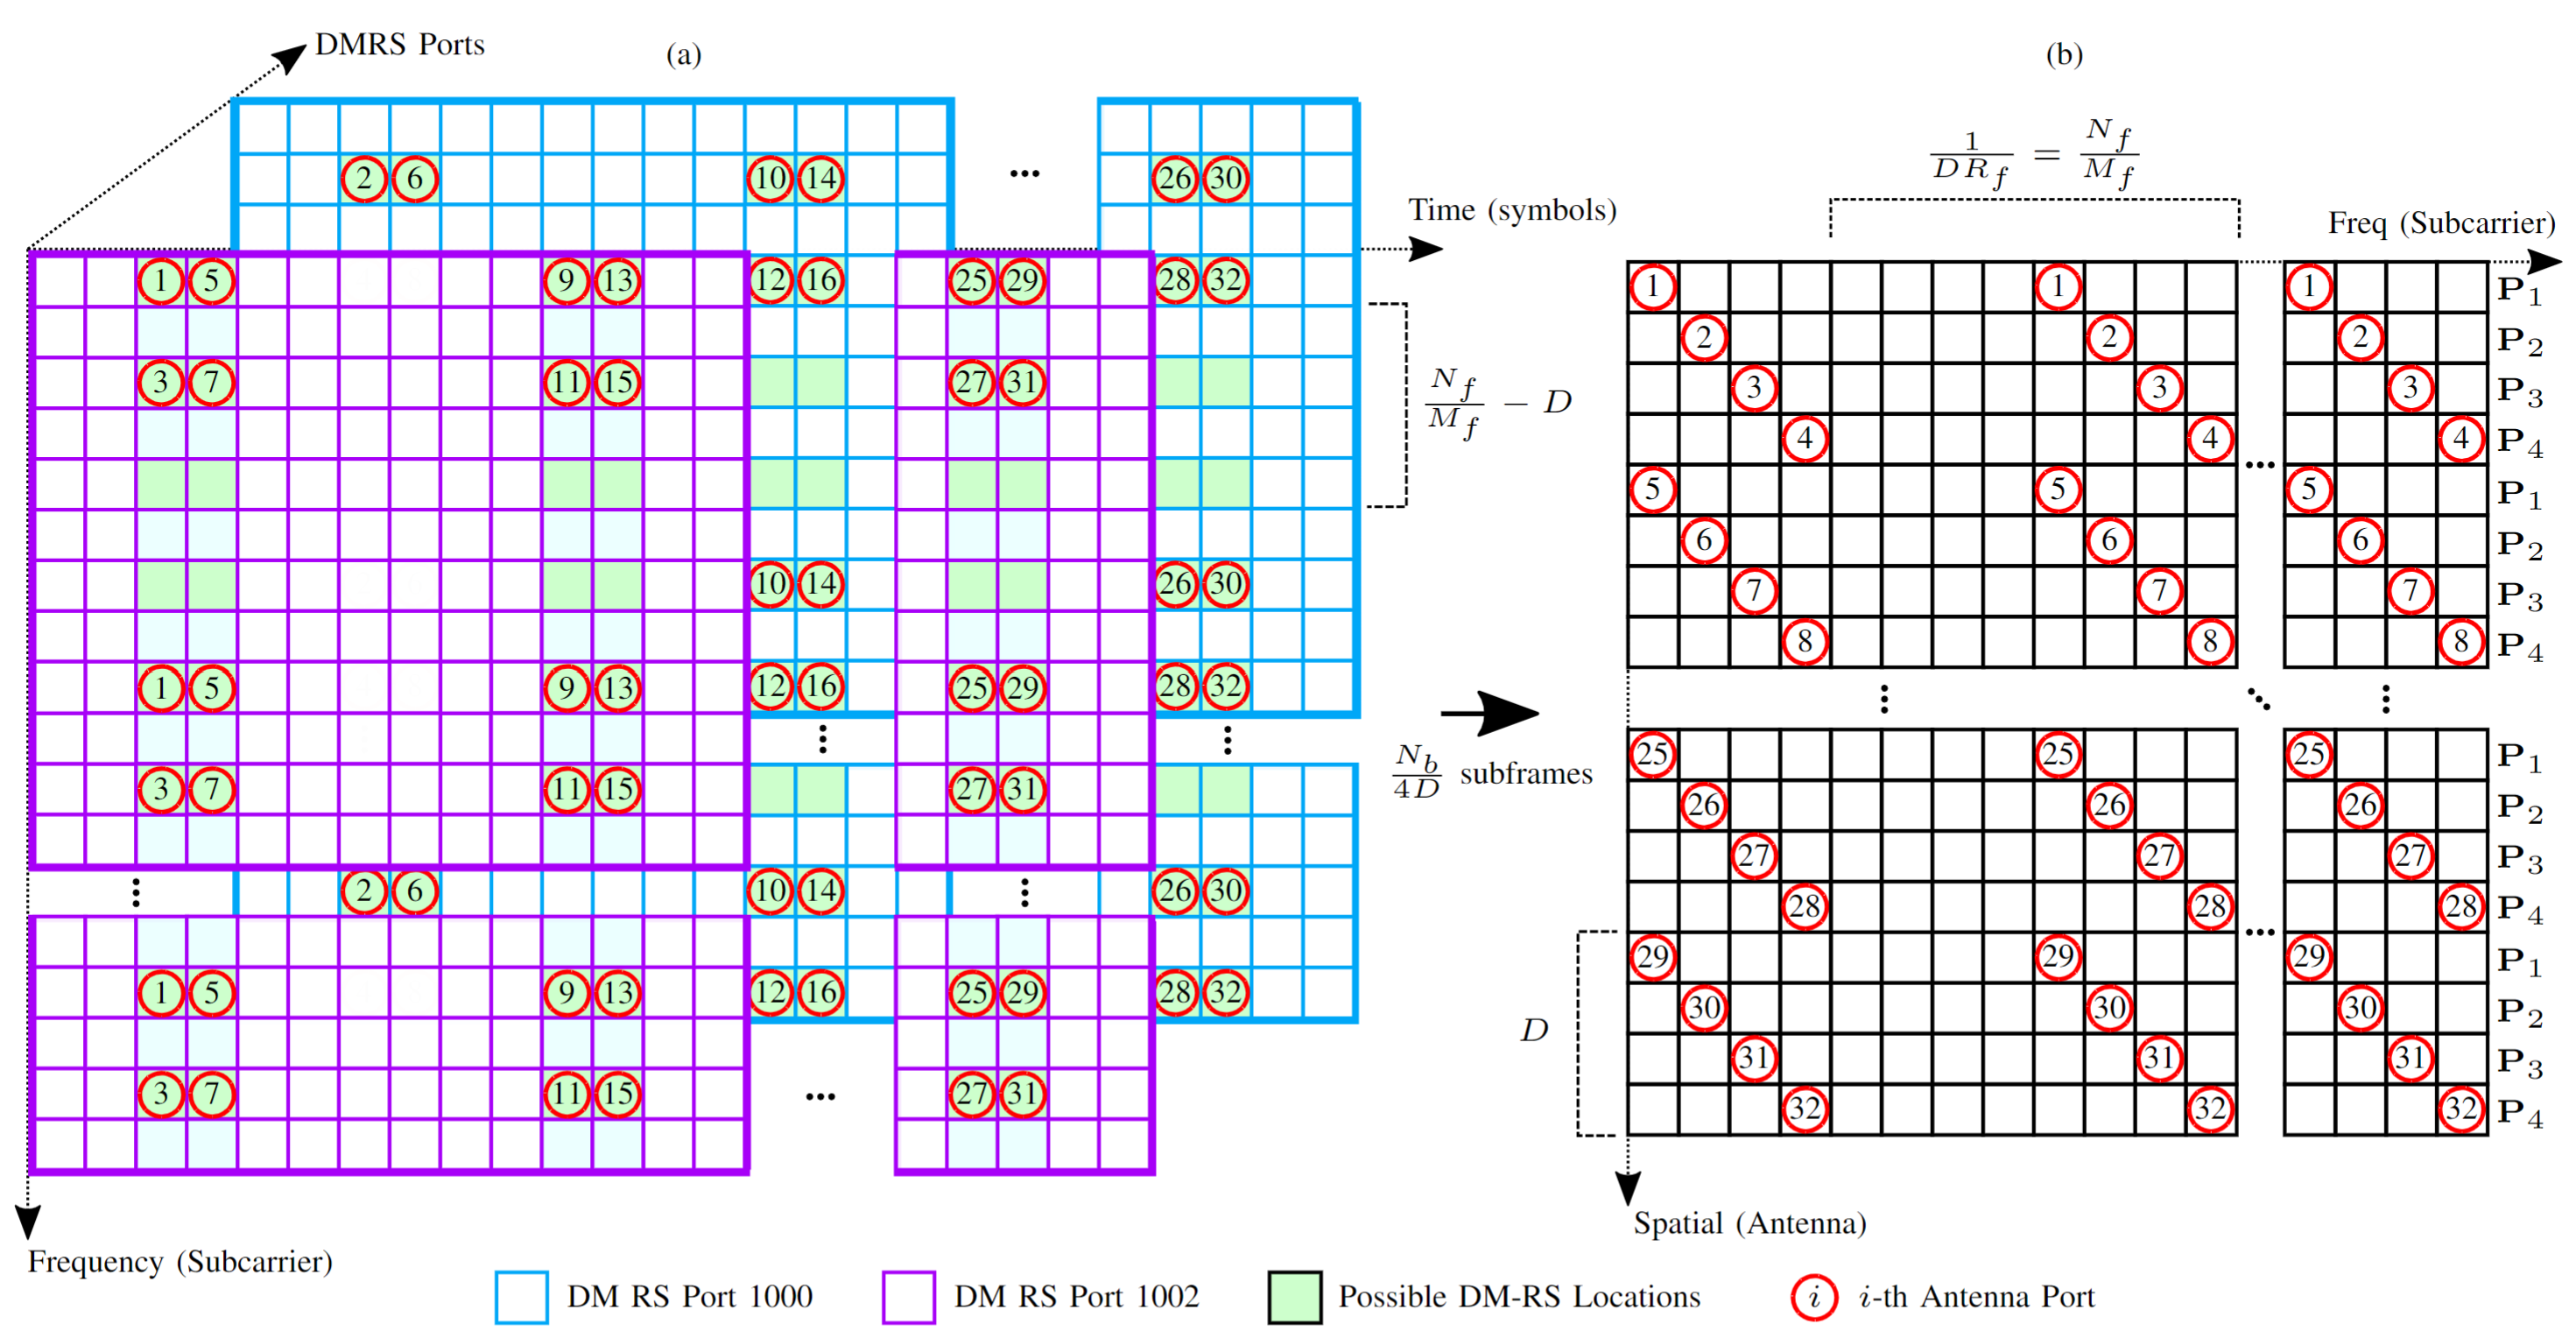
\includegraphics[width=\linewidth]{../images/03_p2d_pilots_diag_with_resource_grid_5gnr_ortho.png}
      % \caption{(a) 5G NR Resource Blocks and DMRS locations. (b) Schematic for diagonal pilots with relevant parameters, size of diagonal $D$ and frequency downsampling ratio $\text{DR}_f$. In this diagram, $N_b=32, D=4, \text{DR}_f=\frac 18$. Pilot matrix $\mathbf{P}_j$ gives downsampling pattern for the $j$-th element of the diagonal pattern.}
      \label{fig:p2d_diag_5gnr}
    \end{figure}
    }
  \end{frame}
  }

  \nofoot{
  \begin{frame}{Pilots-to-Delay Estimator (P2DE)}
    \footnotesize{
    Algorithm~\ref{alg:p2d-diag} outlines the process for acquiring truncated delay domain from sparse/downsampled frequency domain pilots.
    }
    \begin{algorithm}[H]
      {\fontsize{8}{8}\selectfont
      \caption{Pilots-to-delay Estimator (P2DE) for Diagonal Pilot Pattern} 
      \label{alg:p2d-diag}
      \begin{algorithmic}
        \State \textbf{\emph{Input}}:
            P2DE Matrices, $\mathbf{Q}_{c,j}^\#,\;
            j\in\{1,\dots, D\}$
        \State \textbf{\emph{Input}}: Pilot spatial-frequency CSI, $\mathbf{H}_d\in\mathbb{C}^{N_b\times M_f}$
        \State \textbf{\emph{Initialize}}: Spatial-delay CSI, $\tilde{\mathbf{H}}_\tau\in\mathbb{C}^{N_b\times N_t}$
       \State \textbf{\emph{Initialize}}: Angular-delay CSI estimate, ${\mathbf{H}}_\tau
                  \in\mathbb{C}^{N_b\times N_t}$
       \For {$i=1,2,\ldots, N_b$}
            \State \textbf{\# \emph{Index for $j$-th pilot matrix}}
            \State $j = ((i-1) \text{ mod } D) + 1$
            \State \textbf{\# \emph{Apply P2D to $i$-th antenna port}}
            \State ${\boldeta}_{d,i} = \mathbf{H}_d(i,:)$
            \State $\tilde{{\mathbf{H}}}_{\tau}(i,:) = {\boldeta}_{d,i}\mathbf{Q}^{\#}_{c,j}$
            \EndFor
            \State \textbf{\# \emph{Convert from spatial to angular}}
            \State ${{\mathbf{H}}}_{\tau}=\mathbf{F}_{N_b}\tilde{{\mathbf{H}}}_{\tau}$
            \State \textbf{\emph{Return}} ${{\mathbf{H}}}_{\tau}$
      \end{algorithmic} 
      } % \fontsize
    \end{algorithm}
  \end{frame}
  }

  \begin{frame}{Pilots-to-Delay Estimator (P2DE)}
    \begin{figure}[!hbtp]
    \centering
    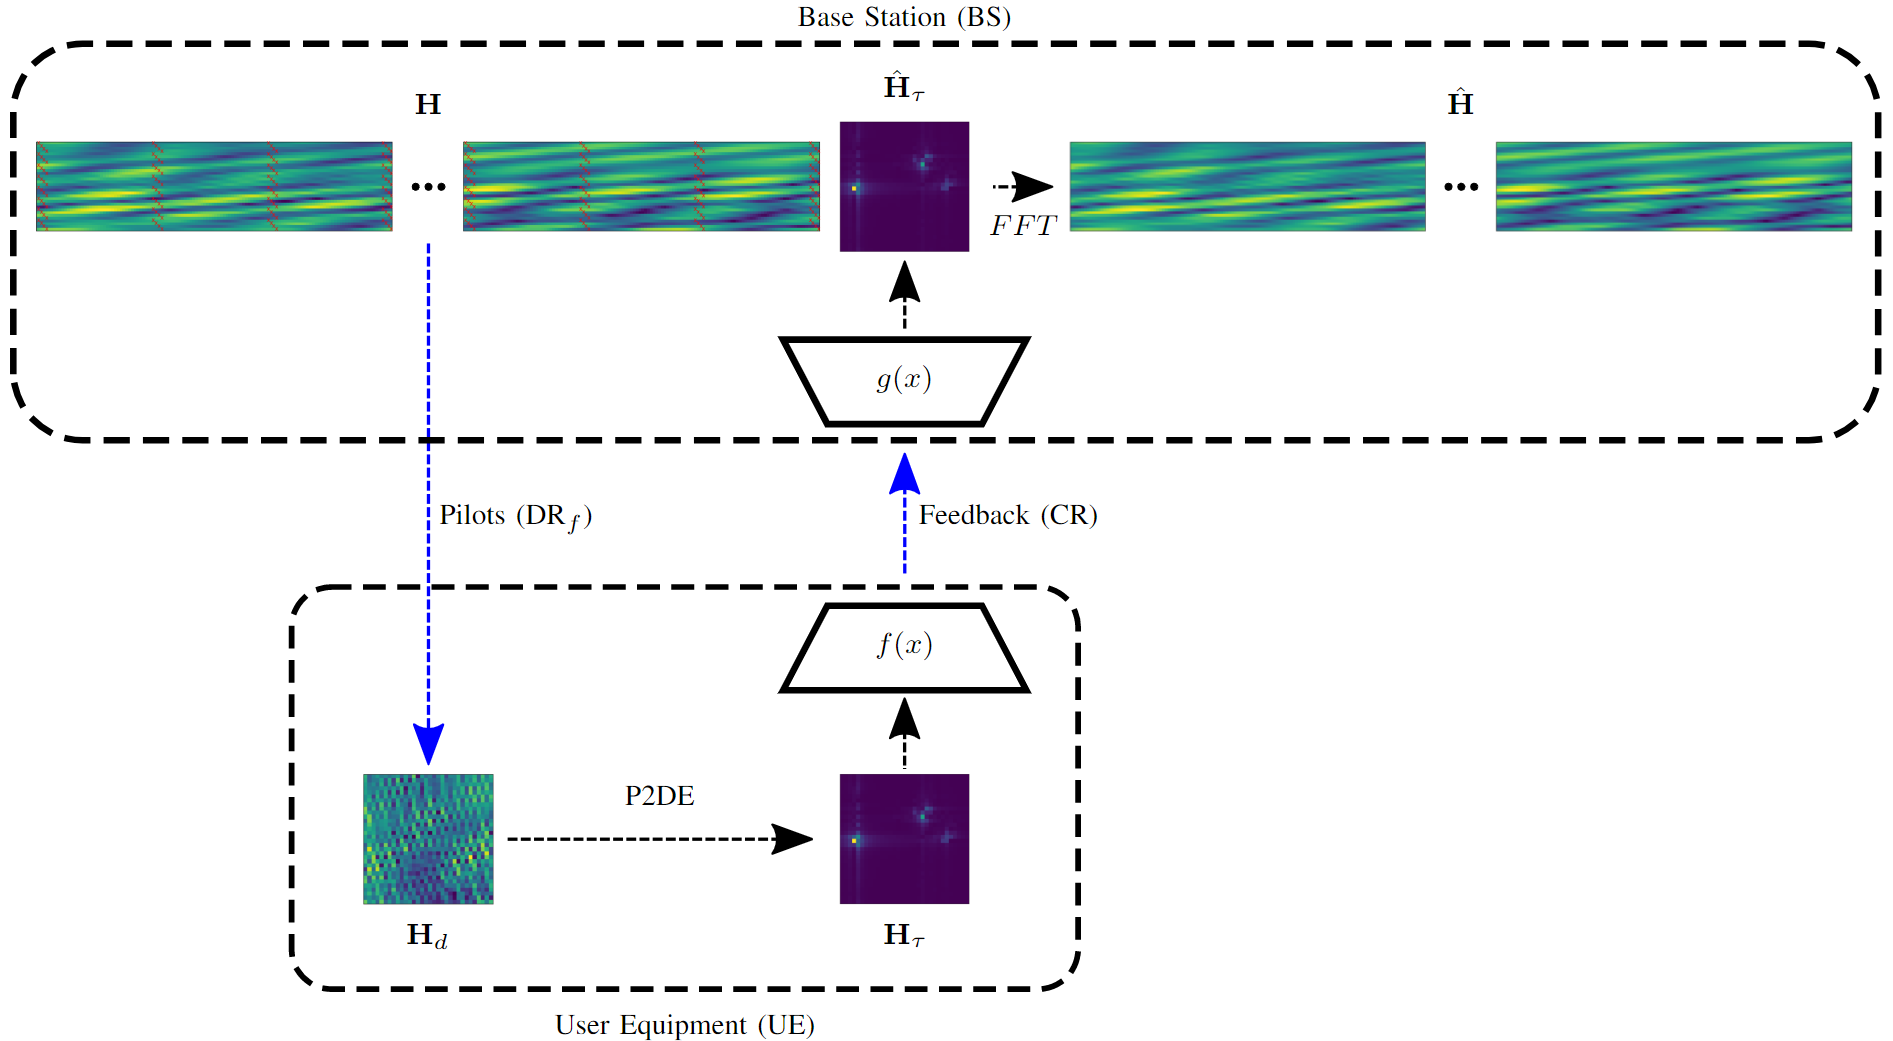
\includegraphics[width=\linewidth]{../images/00_downlink_p2d_feedback_horiz_diag.png}
    \label{fig:p2d}
    \end{figure}
  \end{frame}

  \nofoot{
  \begin{frame}{P2DE Results: Frequency Downsampling Rate}
    Assess the accuracy of the P2DE at the UE (i.e., before compression and feedback) for different frequency downsampling ratios.
    \begin{figure}[!hbtp]
        \centering
        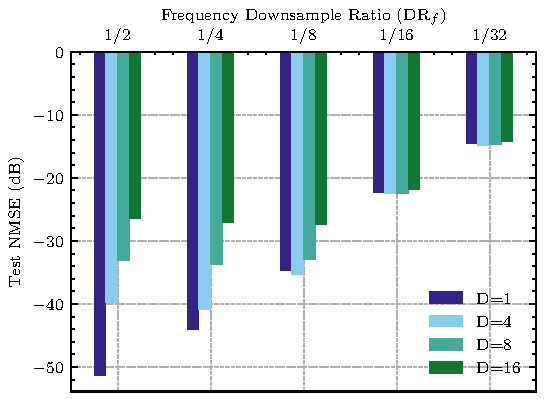
\includegraphics[width=0.8\linewidth]{../images/outdoor_p2d_diag.pdf}
        % \caption{P2D estimation performance under different frequency downsampling ratios ($\text{DR}_f=\frac{M_f}{N_f}$) and diagonal dimensions ($D$) for the Outdoor COST2100 dataset. Downsampling is done along the frequency axis.}
        \label{fig:outdoor_p2d_init}
    \end{figure}
  \end{frame}
  }

  \nofoot{
  \begin{frame}{P2DE with Differential Encoding}
    Differential encoding network using P2DE at the UE.
    \begin{figure}[!hbtp]
      \centering
      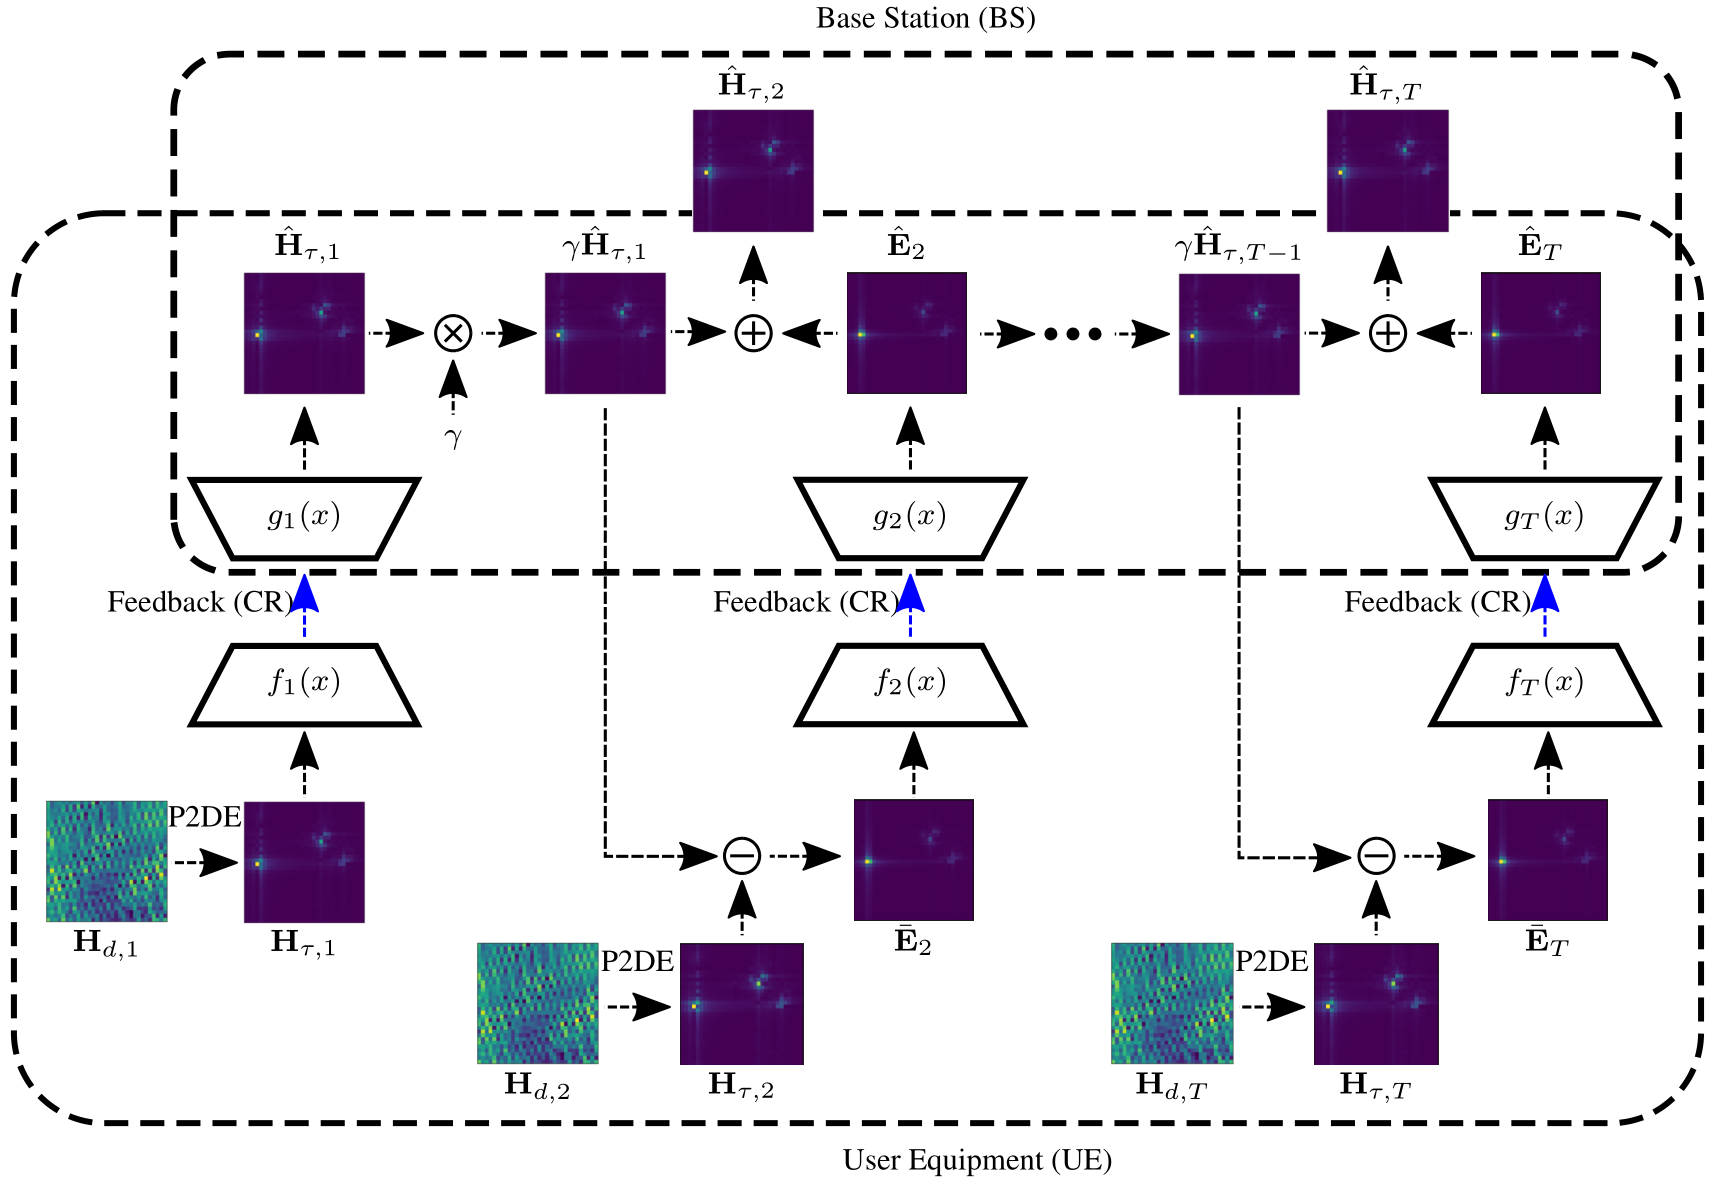
\includegraphics[width=0.9\linewidth]{../images/02_markov_ista_p2d.png}
      % \caption{Diagram of a CSI estimation network using compressed differential feedback based on the linear P2DE. First, downlink pilots are used to estimate a downsampled frequency domain CSI estimate, $\bar{\mathbf{H}}_t\in\mathbb{C}^{N_b \times M_f}$ where $M_f << N_f$ at the $t$-th timeslot. Then, the P2DE $\mathbf{Q}^\#_{N_t}$ of Algorithm~\ref{alg:p2d-diag} is applied to estimate $\tilde{\mathbf{H}}_t$. After P2DE, the learnable transforms $f_t(x)$ and $g_t(x)$ are used to compress and decode the feedback, respectively. For $t=1$, the encoder/decoder are applied directly to $\tilde{\mathbf{H}}_1$. In all subsequent timeslots ($t > 1$), the differential term $\mathbf{E}_t$ is compressed and fed back.}
      % \label{fig:markov-p2d}
    \end{figure}
  \end{frame}
  }

  \nofoot{
  \begin{frame}{Heterogeneous Differential Encoding}
    % \begin{columns}
    %   \begin{column}{0.4\textwidth}
    \footnotesize{
    \begin{itemize}
      \item \textbf{Homogeneous:} MarkovNet used the same network at each timeslot (CsiNet Pro). 
      \item \textbf{Heterogeneous:} Use different networks at different timeslots.
    \end{itemize}
    }
      % \end{column}
      % \begin{column}{0.6\textwidth}
    \begin{figure}[!hbtp]
      \centering
      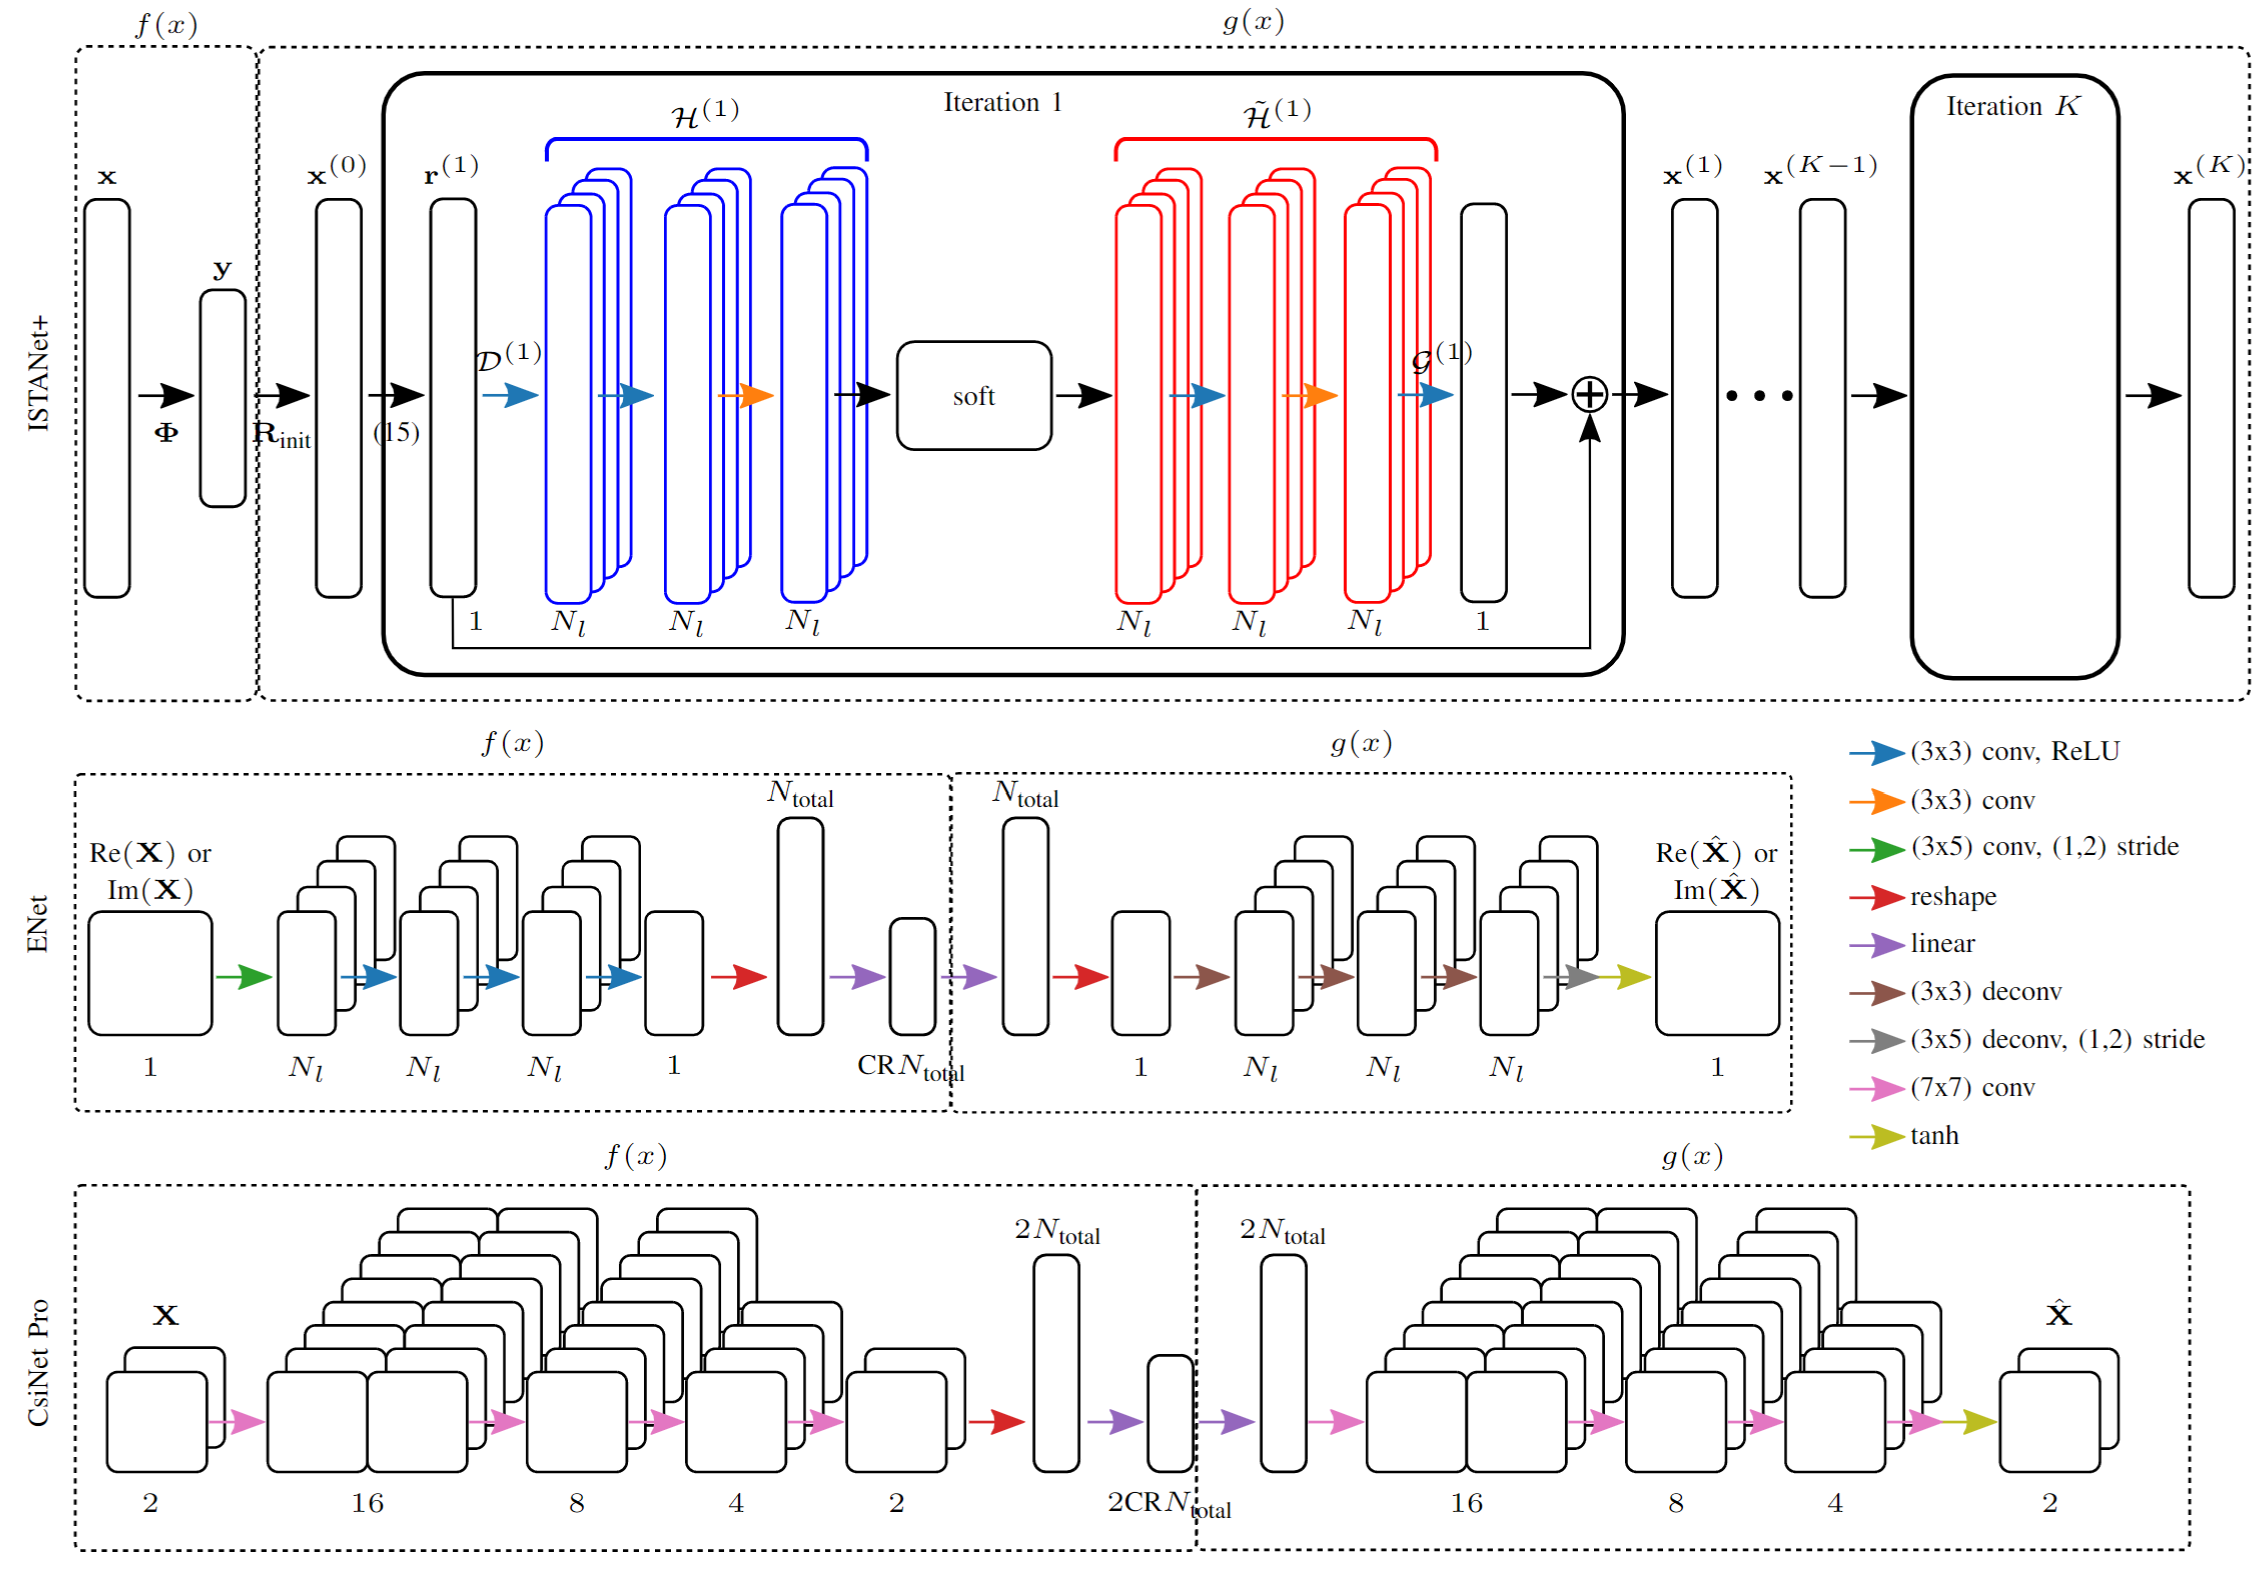
\includegraphics[width=0.8\linewidth]{arch-comparison.png}
      % \caption{Compressive CSI estimation architectures used in this work. $f(x)$ denotes the encoder, and $g(x)$ denotes the decoder. $N_{\text{total}}=N_bN_t$ is the size of the real or imaginary channel. $N_l$ is the number of latent channels in a convolutional layer.}
      \label{fig:arch_compare}
    \end{figure}
    %   \end{column}
    % \end{columns}
  \end{frame}
  }

  \nofoot{
  \begin{frame}{P2DE Results: Compression Network Comparison}
    \footnotesize{
    \begin{columns}
      \begin{column}{0.4\textwidth}
          \begin{itemize}
            \item Single timeslot performance of networks.
            \item Deep CS network (ISTANet+) can outperform autoencoder approaches (ENet, CsiNet Pro)
            \item ENet can outperform CsiNet Pro
          \end{itemize}
      \end{column}
      \begin{column}{0.6\textwidth}
        \begin{figure}[!hbtp]
          \centering
          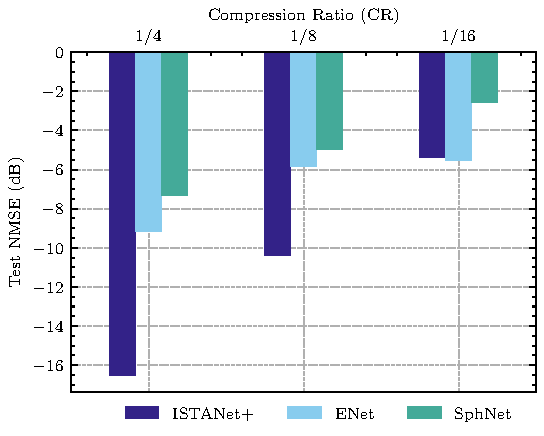
\includegraphics[width=\columnwidth]{outdoor_net_compare.pdf}
          \caption{Performance comparison for different feedback compression networks using P2D estimates ($\text{DF}_f=1/16, D=4$) for Outdoor COST2100 dataset.}% For all tested networks, we use $N_{\text{phase}}=4$, resulting in an augmented training set with $80$k samples.}
          \label{fig:outdoor_net_ablation}
        \end{figure}
      \end{column}
    \end{columns}
    }
  \end{frame}
  }

  \begin{frame}{Heterogeneous Differential Encoding}
    \footnotesize{
    Three different configurations:
    \begin{itemize}
      \item \textbf{MarkovNet-ISTA (MN-I):} \emph{Homogeneous} MarkovNet using ISTANet+ at all timeslots ($t_1$, $t_2$, \dots, $t_T$). 
      \item \textbf{MarkovNet-ENet (MN-E):} \emph{Homogeneous} MarkovNet using ISTANet+ at all timeslots ($t_1$, $t_2$, \dots, $t_T$).
      \item \textbf{MarkovNet-ISTA-ENet (MN-IE):} \emph{Heterogeneous} MarkovNet using ISTANet+ at $t_1$ and ENet at all other timeslots ($t_2$, $t_3$, \dots, $t_T$). 
    \end{itemize}
    }
  \end{frame}

  \nofoot{
  \begin{frame}{Heterogeneous Differential Encoding: Results}
    \footnotesize{
    % \begin{columns}
    %   \begin{column}{0.4\textwidth}
    %       \begin{itemize}
    %         \item Homogeneous 
    %         \item Deep CS network (ISTANet+) can outperform autoencoder approaches (ENet, CsiNet Pro)
    %         \item ENet can outperform CsiNet Pro
    %       \end{itemize}
    %   \end{column}
    %   \begin{column}{0.6\textwidth}
        \begin{figure}[!hbtp]
          \centering
          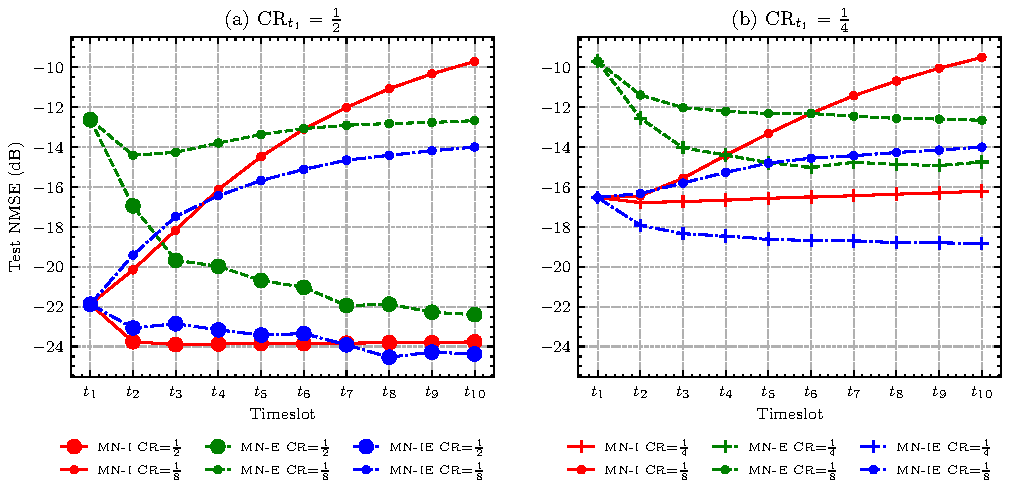
\includegraphics[width=\linewidth]{outdoor_markov_sweep_v2.pdf}
          \caption{Compressive CSI estimation using differential encoding and linear P2D estimator ($M_f=128, \text{DR}_f=\frac{1}{8}, D=4$). MarkovNet-ISTA (MN-I), MarkovNet-ENet (MN-E), and MarkovNet-ISTA-ENet (MN-IE) are tested using two different compression ratios in the first timeslot, $\text{CR}_{t_1}\in\left[\frac{1}{2},\frac{1}{4}\right]$.}
          \label{fig:markov-p2d-results}
        \end{figure}
    %   \end{column}
    % \end{columns}
    }
  \end{frame}
  }

  \nofoot{
  \begin{frame}{Heterogeneous Differential Encoding: Complexity}
    \footnotesize{
    \begin{table}[htb]
    \centering
    \caption{Computational complexity of networks used in this work (lower is better). \textbf{Bold face} in a column indicates lowest value for given compression ratio.} % ``CR" $=$ compression ratio, ``Enc" $=$ encoder, ``Dec" $=$ decoder. FLOPs indicate computation during inference (i.e., not training/back-propagation).}
    \label{tab:net-complexity} 
    \begin{tabular}{|cc|cccc|cc|}
    \hline
    \multicolumn{2}{|c|}{\multirow{2}{*}{}}                    & \multicolumn{4}{c|}{Parameters (M)}                                                                                          & \multicolumn{2}{c|}{\multirow{2}{*}{FLOPs (M)}}     \\ \cline{3-6}
    \multicolumn{2}{|c|}{}                                     & \multicolumn{2}{c|}{Trainable}                                          & \multicolumn{2}{c|}{All}                           & \multicolumn{2}{c|}{}                               \\ \hline
    \multicolumn{1}{|c|}{}                            & CR     & \multicolumn{1}{c|}{Enc}           & \multicolumn{1}{c|}{Dec}           & \multicolumn{1}{c|}{Enc}           & Dec           & \multicolumn{1}{c|}{Enc}           & Dec            \\ \hline
    \multicolumn{1}{|c|}{\multirow{4}{*}{ISTANet+}}    & $1/2$  & \multicolumn{1}{c|}{\textbf{0.00}} & \multicolumn{1}{c|}{\textbf{0.34}} & \multicolumn{1}{c|}{2.10}          & 4.54          & \multicolumn{1}{c|}{\textbf{2.10}} & 393.78         \\ \cline{2-8} 
    \multicolumn{1}{|c|}{}                            & $1/4$  & \multicolumn{1}{c|}{\textbf{0.00}} & \multicolumn{1}{c|}{0.34}          & \multicolumn{1}{c|}{1.05}          & 2.44          & \multicolumn{1}{c|}{\textbf{1.05}} & 373.85         \\ \cline{2-8} 
    \multicolumn{1}{|c|}{}                            & $1/8$  & \multicolumn{1}{c|}{\textbf{0.00}} & \multicolumn{1}{c|}{0.34}          & \multicolumn{1}{c|}{0.52}          & 1.39          & \multicolumn{1}{c|}{\textbf{0.52}} & 363.89         \\ \cline{2-8} 
    \multicolumn{1}{|c|}{}                            & $1/16$ & \multicolumn{1}{c|}{\textbf{0.00}} & \multicolumn{1}{c|}{0.34}          & \multicolumn{1}{c|}{0.26}          & 0.87          & \multicolumn{1}{c|}{\textbf{0.26}} & 358.91         \\ \hline
    \multicolumn{1}{|c|}{\multirow{4}{*}{ENet}}       & $1/2$  & \multicolumn{1}{c|}{0.55}          & \multicolumn{1}{c|}{0.55}          & \multicolumn{1}{c|}{\textbf{0.55}} & \textbf{0.55} & \multicolumn{1}{c|}{29.98}         & 29.70          \\ \cline{2-8} 
    \multicolumn{1}{|c|}{}                            & $1/4$  & \multicolumn{1}{c|}{0.29}          & \multicolumn{1}{c|}{\textbf{0.29}} & \multicolumn{1}{c|}{\textbf{0.29}} & \textbf{0.29} & \multicolumn{1}{c|}{29.46}         & 29.18          \\ \cline{2-8} 
    \multicolumn{1}{|c|}{}                            & $1/8$  & \multicolumn{1}{c|}{0.16}          & \multicolumn{1}{c|}{\textbf{0.16}} & \multicolumn{1}{c|}{\textbf{0.16}} & \textbf{0.16} & \multicolumn{1}{c|}{29.20}         & 28.92          \\ \cline{2-8} 
    \multicolumn{1}{|c|}{}                            & $1/16$ & \multicolumn{1}{c|}{0.09}          & \multicolumn{1}{c|}{\textbf{0.09}} & \multicolumn{1}{c|}{\textbf{0.09}} & \textbf{0.09} & \multicolumn{1}{c|}{29.07}         & 28.79          \\ \hline
    \multicolumn{1}{|c|}{\multirow{4}{*}{CsiNet Pro}} & $1/2$  & \multicolumn{1}{c|}{1.06}          & \multicolumn{1}{c|}{1.06}          & \multicolumn{1}{c|}{1.06}          & 1.06          & \multicolumn{1}{c|}{12.16}         & \textbf{12.16} \\ \cline{2-8} 
    \multicolumn{1}{|c|}{}                            & $1/4$  & \multicolumn{1}{c|}{0.53}          & \multicolumn{1}{c|}{0.53}          & \multicolumn{1}{c|}{0.53}          & 0.53          & \multicolumn{1}{c|}{11.11}         & \textbf{11.11} \\ \cline{2-8} 
    \multicolumn{1}{|c|}{}                            & $1/8$  & \multicolumn{1}{c|}{0.27}          & \multicolumn{1}{c|}{0.27}          & \multicolumn{1}{c|}{0.27}          & 0.27          & \multicolumn{1}{c|}{10.59}         & \textbf{10.59} \\ \cline{2-8} 
    \multicolumn{1}{|c|}{}                            & $1/16$ & \multicolumn{1}{c|}{0.14}          & \multicolumn{1}{c|}{0.14}          & \multicolumn{1}{c|}{0.14}          & 0.14          & \multicolumn{1}{c|}{10.33}         & \textbf{10.33} \\ \hline
    \end{tabular}
    \end{table}
    }
  \end{frame}
  }

  \begin{frame}{Heterogeneous Differential Encoding: Conclusions}
    \begin{itemize}
      \item Deep CS network (ISTANet+) can provide superior initial estimate with slightly more complexity.
      \item Autoencoder network (ENet) can provide good error compression/estimation.
      \begin{itemize}
        \item Fewer encoder/decoder parameters
        \item More encoder FLOPs, less decoder FLLOPs
      \end{itemize}
    \end{itemize}
  \end{frame}

\section{Current Work: Pilot Feedback and Model Re-use}

  % Background section frame 
  \begin{frame}[plain]
    \vfill
    \centering
    \begin{beamercolorbox}[sep=8pt,center,shadow=true,rounded=true]{Direct Frequency Feedback and Model Re-use}
      \usebeamerfont{title}\insertsectionhead\par%
      \color{davisblue}\noindent\rule{10cm}{1pt} \\
      \footnotesize{UE-focused reduction of complexity of CSI feedback.} 
      % \LARGE{\faFileTextO}
    \end{beamercolorbox}
    \vfill
  \end{frame}


  \nofoot{
  \begin{frame}{P2DE: UE-side Computation}
    \footnotesize{
    \begin{figure}[!hbtp]
      \centering
      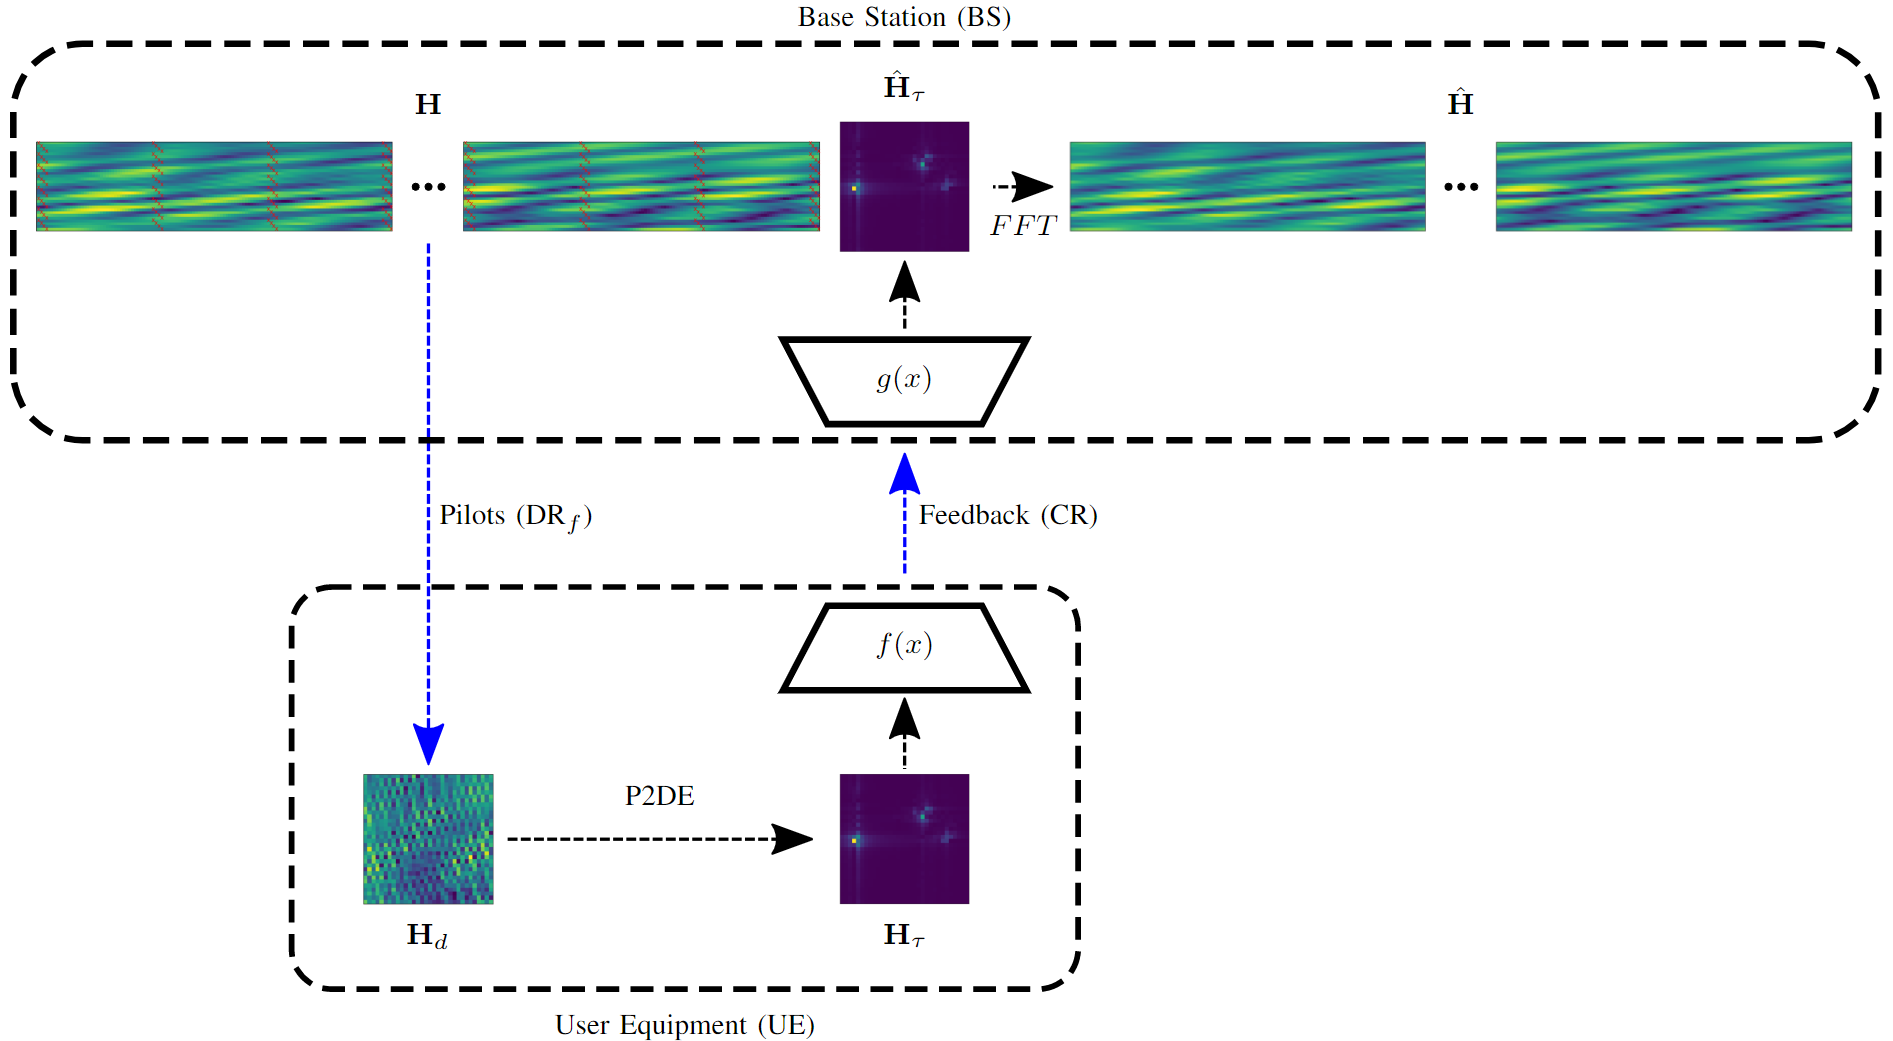
\includegraphics[width=\linewidth]{../images/00_downlink_p2d_feedback_horiz_diag.png}
      \label{fig:p2d}
    \end{figure}
    \textbf{Problem:} Encoder computation at (low-resourced) UE. Can we reduce this?
    }
  \end{frame}
  }

  \begin{frame}{P2DE: UE-side Computation}
    \begin{table}[!h]
      \caption{Computational complexity of P2DE for $D=1$ (diagonal pattern size), $N_f=1024$ (number of subcarriers), and $N_b=32$ (\# antennas in ULA).}
      \begin{center}
      \label{tab:p2de-comp} 
      \begin{tabular}{|r|c|c|c|}
      \hline
      $\mathbf{M_f}$      & $\mathbf{32}$      & $\mathbf{64}$       & $\mathbf{128}$     \\ \hline
      \textbf{FLOPs}      & $1.05\cdot 10^{6}$ & $2.10\cdot 10^{6}$  & $4.19\cdot 10^{6}$ \\ \hline
      \textbf{Parameters} & $6.55\cdot 10^{4}$ & $1.31\cdot 10^{5}$  & $2.62\cdot 10^{5}$  \\ \hline
      \end{tabular}
      \end{center}
      \vspace*{-0.3mm}
    \end{table}
  \end{frame}

  \begin{frame}{Pilot-based Feedback}
    \begin{figure}[!hbtp]
      \centering
      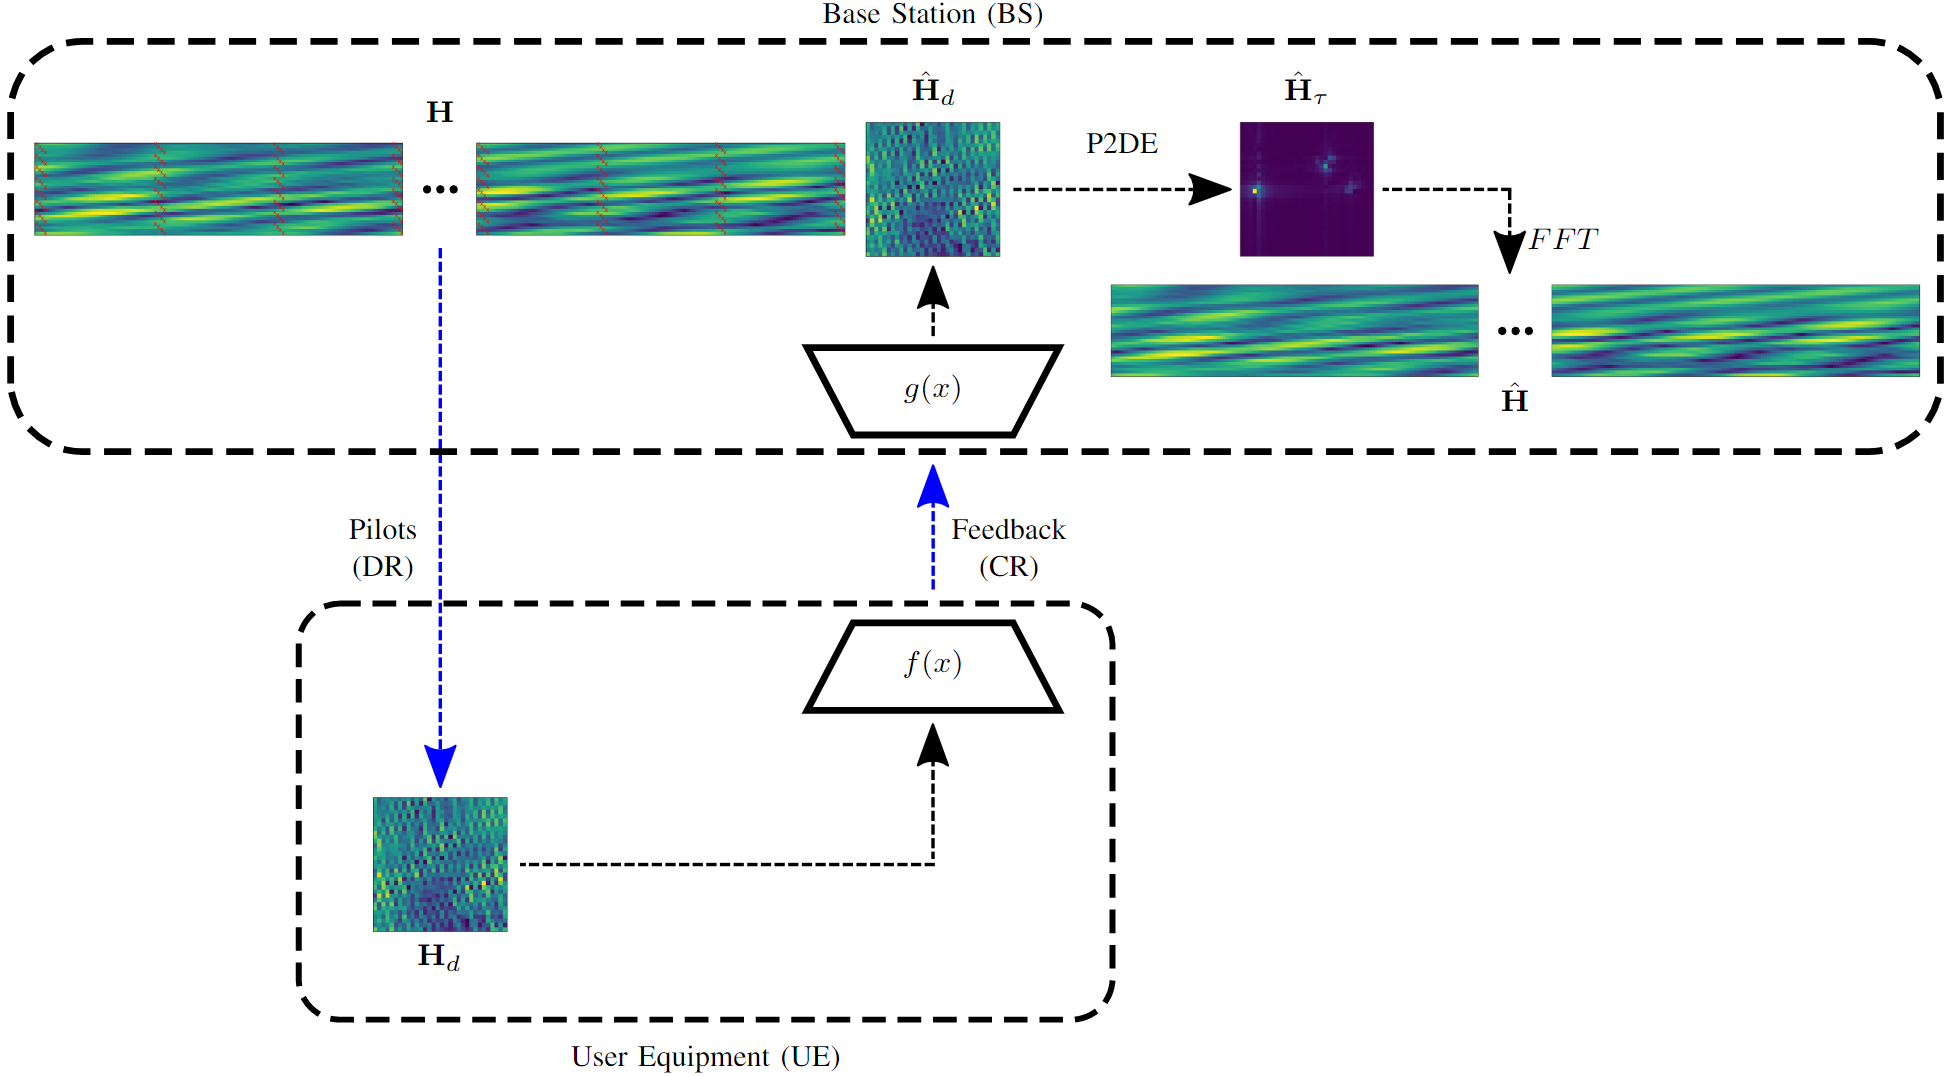
\includegraphics[width=\linewidth]{01_downlink_p2d_direct_feedback_horiz_diag.png}
      \caption{Compressive CSI estimation based on linear P2D estimator on BS side. 
      % First, we use downlink pilots to 
      % generate a sparse, frequency domain CSI
      % estimate 
      % of size $M_f << N_f$. This downsampled frequency domain CSI estimate is compressed at the UE
      % and fed back to the BS.
      % At the BS, we apply
      % the P2D estimator, $\mathbf{Q}^{\#}_{N_t}$ \cite{ref:delRosario2022p2d} to acquire 
      % the truncated
      % delay domain CSI estimate.
      % We train a
      % learnable encoder, 
      % $f(x)$,
      % and decoder, $g(x)$, to compress and decode the feedback, respectively. The 
      % BS recovers
      % the frequency domain
      % CSI from 
      % the decoded 
      % delay domain CSI estimate.
      }
      \label{fig:p2d_direct}
    \end{figure}
  \end{frame}

  \begin{frame}{Model Re-use}
    \begin{figure}
      \centering
      {
        \fontsize{8pt}{8pt}
        \def\svgwidth{1.0\linewidth}
        \input{../images/02_per_K_subc.pdf_tex}
      }
      \caption{Compressive CSI estimation with model re-
      use. % Rather than compressing the entire input, $\mathbf{H}_d$,
      The encoder compresses $K$ contiguous pilot subcarriers
      from the input, resulting in $\frac{M_f}{K}$ payloads of feedback
      (shown in different colors above). 
      % Meanwhile at the
      % BS, the decoder recovers each set of $K$ contiguous
      % subcarriers based on the $\frac{M_f}{K}$ payloads, and the
      % decoded payloads are combined to generate the full
      % frequency domain estimate.
      }
      \label{fig:model_reuse}
    \end{figure}
  \end{frame}

  \begin{frame}{Model Re-use}
    \begin{figure}
      \centering
      {
        \fontsize{8pt}{8pt}
        \def\svgwidth{1.0\linewidth}
        \input{../images/03_per_K_subc_w_flat.pdf_tex}
      }
      % \caption{ISTANet+ with model re-
      % use. % Rather than compressing the entire input, $\mathbf{H}_d$,
      % The $\Phi$ $K$ contiguous pilot subcarriers
      % from the input, resulting in $\frac{M_f}{K}$ payloads of feedback
      % (shown in different colors above). 
      % }
      \label{fig:model_reuse_w_flat}
    \end{figure}
    We use ISTANet+ \cite{ref:zhang2018ista},
    which compresses CSI at UE via, 
    \begin{align}
        f(x) &= \mathbf{\Phi}\mathbf{x}
    \end{align}
    for $\mathbf{x} \in \mathbb{R}^{N_K}$ and $\mathbf{\Phi} \in \mathbb{R}^{\text{CR} N_K  \times N_K}$ where $N_K = 2 K N_b$
  \end{frame}

  \nofoot{
  \begin{frame}{Pilot Feedback + Model Re-use: Results}
    \footnotesize{
      \begin{itemize}
        \item Outdoor (top) and Indoor (bottom) results w.r.t. NMSE vs. complexity (log(FLOPs) on left, parameters on right) using different number of pilot subcarriers ($M_f$).
        \item Compare with P2DE at UE and no model re-use ({\color{red}red}).
      \end{itemize}
    }
    \begin{figure}[!hbtp]
      \centering
      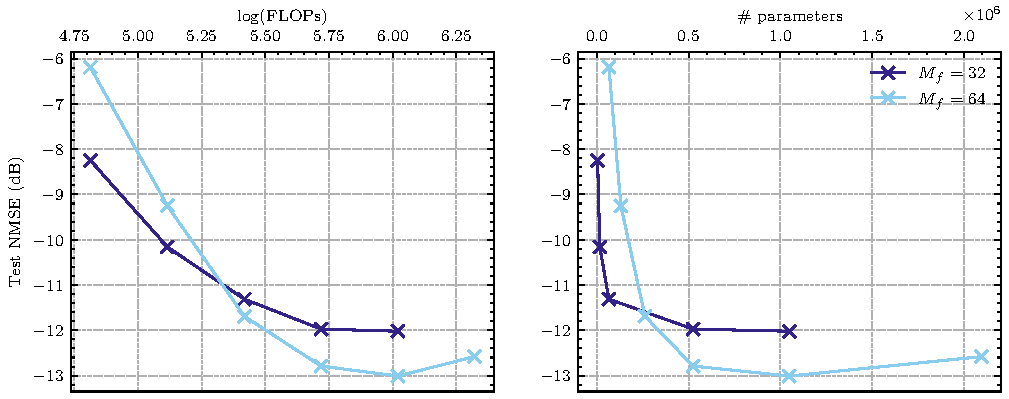
\includegraphics[width=0.65\linewidth]{outdoor_subc_sweep_line.pdf}
      % \caption{NMSE vs. encoder complexity of shared model architectures (i.e., complexity is w.r.t. FLOPs and parameters at UE). Outdoor COST2100 model.}
      \label{fig:outdoor_nmse_vs_complexity}
    \end{figure}

    \begin{figure}[!hbtp]
      \centering
      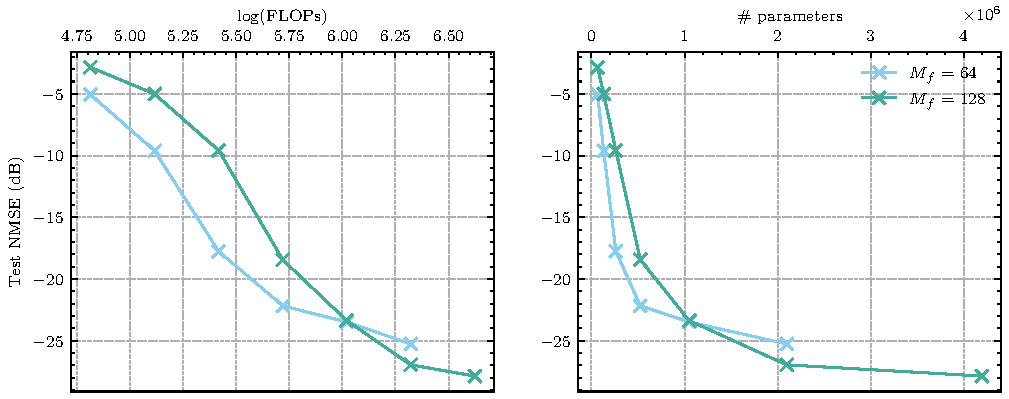
\includegraphics[width=0.65\linewidth]{indoor_subc_sweep_line.pdf}
      % \caption{NMSE vs. encoder complexity for shared model architectures (i.e., complexity is w.r.t. FLOPs and parameters at UE). Indoor COST2100 model.}
      \label{fig:indoor_nmse_vs_complexity}
    \end{figure}
  \end{frame}
  }

  \nofoot{
  \begin{frame}{Pilot Feedback + Model Re-use: Conclusions}
    \footnotesize{
    \begin{itemize}
      \item Indoor: Can maintain same NMSE with 10-fold reduction in FLOPs
      \item Outdoor: NMSE increase of 2.5dB with 10-fold reduction in FLOPs, $10^6$ reduction in parameters
    \end{itemize}
    }

    \begin{figure}[!hbtp]
      \centering
      \includegraphics[width=0.65\linewidth]{outdoor_subc_sweep_line.pdf}
      % \caption{NMSE vs. encoder complexity of shared model architectures (i.e., complexity is w.r.t. FLOPs and parameters at UE). Outdoor COST2100 model.}
      \label{fig:outdoor_nmse_vs_complexity}
    \end{figure}

    \begin{figure}[!hbtp]
      \centering
      \includegraphics[width=0.65\linewidth]{indoor_subc_sweep_line.pdf}
      % \caption{NMSE vs. encoder complexity for shared model architectures (i.e., complexity is w.r.t. FLOPs and parameters at UE). Indoor COST2100 model.}
      \label{fig:indoor_nmse_vs_complexity}
    \end{figure}
  \end{frame}
  }

  \begin{frame}{Papers}
    \footnotesize{
    \begin{itemize}
      \item \bibentry{ref:liu2020sphnet}
      \item \bibentry{ref:Liu2020MarkovNet}
      \item \bibentry{ref:delRosario2022p2d}
      \item \bibentry{ref:delRosario2022directreuse}
    \end{itemize}
    }
  \end{frame}

  \begin{frame}{Acknowledgements}
    \begin{itemize}
      \item Thesis committee
      \pause
      \item Prof. Ding, lab mates, collaborators
      \pause
      \item My parents, my brother
      \pause
      \item My SO
    \end{itemize}
  \end{frame}

\section*{Questions?}
    \begin{frame}[plain]
        \vfill
      \centering
      \begin{beamercolorbox}[sep=8pt,center,shadow=true,rounded=true]{title}
        \usebeamerfont{title}\insertsectionhead\par%
        \small{\url{mdelrosa@ucdavis.edu}}
        \color{davisblue}\noindent\rule{10cm}{1pt} \\
        % \LARGE{\faFileTextO}
      \end{beamercolorbox}
      \vfill
      \begin{figure}[htb] \centering 
        % \includegraphics[width=0.9\linewidth]{batch0_csi_gt.png}
      {
        \fontsize{4pt}{4pt}
        \def\svgwidth{\columnwidth}
        \input{../images/cnns-venn-diagram-contrib-final.pdf_tex}
      }
      % \caption{Areas of \emph{domain knowledge} and corresponding CNNs.}
      \end{figure}
    \end{frame}

\section*{References}
  \nofoot{
  \begin{frame}{References}
    % https://latex.org/forum/viewtopic.php?t=12027
    \setbeamertemplate{bibliography item}[text]
    \bibliographystyle{ieeetr}
    \begingroup 
    \fontsize{4pt}{4pt}
       % \setlength{\bibsep}{4pt}
       % \setstretch{1}
      \bibliography{../cited_works}
      \emph{Note: \textdagger equal contribution}
    \endgroup
  \end{frame}
  }

\section*{Appendix}

  % Appendix section frame 
  \begin{frame}[plain]
    \vfill
    \centering
    \begin{beamercolorbox}[sep=8pt,center,shadow=true,rounded=true]{Appendix}
      \usebeamerfont{title}\insertsectionhead\par%
      \color{davisblue}\noindent\rule{10cm}{1pt} \\
      % \LARGE{\faFileTextO}
    \end{beamercolorbox}
    \vfill
  \end{frame} 

  \begin{frame}{Evaluation Metrics: Accuracy}
    Metrics used:
    \begin{itemize}
      \item \textbf{Normalized Mean-squared Error}
      \begin{align*}
        \text{NMSE} = \frac 1N \sum_{i}^N \frac{\|\mathbf H_i - \hat{\mathbf H}_i \|^2}{\|\mathbf H_i \|^2}
      \end{align*}
      \item \textbf{Cosine Similarity}
      \begin{align*}
          \rho=\frac{1}{N N_{f}} \sum_{i=1}^{N} \sum_{m=1}^{N_{f}} \frac{|\hat{\bar{\mathbf{h}}}_{i,m}^{H} \bar{\mathbf{h}}_{i,m}|}{\|\hat{\bar{\mathbf{h}}}_{i,m}\|\|\bar{\mathbf{h}}_{i,m}\|},
      \end{align*}
    \end{itemize}
  \end{frame}

  \begin{frame}{Training Hyperparameters}
    \footnotesize{
      \textbf{SphNet (and benchmark networks)}
      \begin{itemize}
        \item \textbf{Epochs}: 1000
        \item \textbf{Optimizer}: Adam with learning rate $10^{-3}$
      \end{itemize}
      \textbf{MarkovNet}
      \begin{itemize}
        \item \textbf{Epochs ($t_1$)}: 1000
        \item \textbf{Epochs ($t_2,\dots,t_T$)}: 150
        \item \textbf{Optimizer}: Adam with learning rate $10^{-3}$
        \item Each timeslot is initialized with weights from previous timeslot.
      \end{itemize}
      \textbf{CsiNet-LSTM}
      \begin{itemize}
        \item \textbf{Epochs}: 1000 (pretraining CsiNet), 500 (CsiNet-LSTM)
        \item \textbf{Optimizer}: Adam with learning rate $10^{-3}$
      \end{itemize}
      }
  \end{frame}

  % \begin{frame}{Compressed Sensing: Benchmark Description}
  %   \footnotesize{
  %   \begin{itemize}
  %     \item \textbf{LASSO}:
  %     \begin{itemize}
  %       \item Least Absolute Shrinkage Selection Operator
  %       \item $\min \left(\frac 12\|\mathbf y - \mathbf A \mathbf h\|_2^2 + \lambda_p\|\mathbf h\|_1\right)$
  %     \end{itemize}
  %     \item \textbf{TVAL3}:
  %     \begin{itemize} 
  %       \item Total Variational Augmented Alternating-direction Lagrangian Algorithm
  %       \item $$
  %     \end{itemize}
  %     \item \textbf{BM3D-AMP}:
  %     \begin{itemize} 
  %       \item Block Matching 3D Approximate Message Passing
  %       \item $$
  %     \end{itemize}
  %   \end{itemize}
  % \end{frame}

  \nofoot{
  \begin{frame}{BM3D-AMP: Iterative Solution}
    % \begin{columns}
      % \begin{column}{0.5\linewidth}
      % \end{column}
      % \begin{column} {0.5\linewidth}
      \footnotesize{
        D-AMP = Denoising approximate message passing.
        Initialize $x^0 = \mathbf 0,$ and alternate between:
        \begin{align*}
          x^{t+1} &= D_{\hat \sigma^t} (x^t + \mathbf A^*z^t) \\
          z^{t}   &= y - \mathbf A x^{t} + z^{t-1}\frac{\text{div}D_{\hat \sigma^{t-1}} (x^{t-1} + \mathbf A^*z^{t-1})}{m} \\
        \end{align*}
        where $\hat \sigma^t = \text{Var}(x^t + \mathbf A^*z^t)$, $D_{\hat\sigma_t}=$ denoising algorithm.
        \begin{figure}[htb]    
          \centering
          \includegraphics[width=.4\textwidth]{d-amp-subspaces.png}
          \label{fig:d-amp-subspaces}
          \caption{Subspaces of interest in D-AMP.}
        \end{figure}
        }
      % \end{column}
    % \end{columns}
  \end{frame}
  }

  \begin{frame}{BM3D-AMP: Definition}
  \footnotesize{
    BM3D-AMP = D-AMP with \emph{block matching 3D collaborative filtering (BM3D)}.
    \begin{itemize}
      \item Combination of non-local means (NLM) and wavelet thresholding.
      \item Procedure:
      \begin{enumerate}
        \item Compare patches of pixels in images
        \item Group similar patches
        \item 2D (DCT or Bior Wavelet) + 1D Haar wavelet transforms on group
        \item Shrink coefficients in groups ($N \to M$)
        \item Perform inverse transform by 1) hard thresholding and 2) Wiener filter ($M\to N$)
      \end{enumerate}
    \end{itemize}
    }
  \end{frame}

  \begin{frame}{Tanh Normalization}
    Given mean $\mu$, standard deviation $\sigma$ w.r.t $\mathbf H$,
    \begin{align*} 
      H_{\tanh}(i,j) &= \tanh\left(\frac{H(i,j) - \mu}{2\nu\sigma}\right) + 1.
    \end{align*}
    Scale parameter $\nu$ chosen by designer.
  \end{frame}

  \nofoot{
  \begin{frame}{COST2100 (Indoor): Tanh Normalization}
    % Tanh normalization $\to$ larger variance. 
    \begin{figure}[htb]    
      \subfigure[$\nu=1$] {\label{fig:indoor_nu1} 
      \includegraphics[width=.6\textwidth]{cost2100_indoor_tanh_nu1_dist.pdf}
      }
      \subfigure[$\nu=3$] {\label{fig:indoor_nu3} 
      \includegraphics[width=.6\textwidth]{cost2100_indoor_tanh_nu3_dist.pdf}
      }
      \caption{Distribution/variance of indoor COST2100 real/imaginary channels under tanh normalization ($N=9.9\dot 10^5$).}
      \label{fig:cost_indoor_tanh_dist}
    \end{figure}
  \end{frame} 
  }  

  \nofoot{
  \begin{frame}{COST2100 (Outdoor): Tanh Normalization}
    % Tanh normalization $\to$ larger variance. 
    \begin{figure}[htb]    
      \subfigure[$\nu=1$] {\label{fig:outdoor_nu1} 
      \includegraphics[width=.6\textwidth]{cost2100_outdoor_tanh_nu1_dist.pdf}
      }
      \subfigure[$\nu=3$] {\label{fig:outdoor_nu3} 
      \includegraphics[width=.6\textwidth]{cost2100_outdoor_tanh_nu3_dist.pdf}
      }
      \caption{Distribution/variance of outdoor COST2100 real/imaginary channels under tanh normalization ($N=10^5$).}
      \label{fig:cost_outdoor_tanh_dist}
    \end{figure}
  \end{frame} 
  }  

  \begin{frame}{Multivariate Autoregression (MAR)}
    Rather than scalar $\hat\gamma \in \mathbb R^+$, we can derive a multivariate $p$-step predictor, $\mathbf W_1, \dots, \mathbf W_p$.
    Given $p$ prior CSI samples, the mean-square optimal predictor
    $\hat H_t$ is a linear combination of these the prior CSI samples,
    \begin{equation}
    \mathbf{\hat H}_{t} = \mathbf{H}_{t-1} \mathbf W_{1} + \dots + \mathbf{H}_{t-p} \mathbf W_{p} + \mathbf E_t.
    \end{equation}
  \end{frame}

  \begin{frame}{Multivariate Autoregression (MAR)}
    Error terms are uncorrelated with the CSI samples
    (i.e. $\mathbf H_{t-i}^H \mathbf E_t = 0$ for all $i \in [0, \dots, p]$),
    and we pre-multiply by $\mathbf H_{t-i}^H$,
    \begin{align}
    \mathbf{H}_{t-i}^H\mathbf{\hat H}_{t} &= \mathbf{H}_{t-i}^H\mathbf{H}_{t-1} \mathbf W_{1} + \dots + \mathbf{H}_{t-i}^H\mathbf{H}_{t-p} \mathbf W_{p} + \mathbf{H}_{t-i}^H\mathbf E_t \nonumber \\
                        &= \mathbf{H}_{t-i}^H\mathbf{H}_{t-1} \mathbf W_{1} + \dots + \mathbf{H}_{t-i}^H\mathbf{H}_{t-p} \mathbf W_{p}. \label{eq:var-init}
    \end{align}
  \end{frame}

  \begin{frame}{Multivariate Autoregression (MAR)}
    Denote the correlation matrix 
    $\mathbf R_i = \mathbb E [\mathbf H^H_{t-i}\mathbf H_{t}]$.
    Presume CSI matrices arise from a 
    stationary process, implying the following properties:
    \begin{enumerate}
      \item $\mathbf R_i = \mathbb E [\mathbf H^H_{t-i}\mathbf H_{t}] = \mathbb E [\mathbf H^H_{t}\mathbf H_{t+i}]$
      \item $\mathbf R_i = \mathbf R^H_{-i}$
    \end{enumerate}
  \end{frame}

  \begin{frame}{Multivariate Autoregression (MAR)}
    Taking the expectation, write (\ref{eq:var-init})
    as a linear combination of $\mathbf R$,
    \begin{align*}
    \mathbf R_{i+1} &= \mathbf{R}_{i} \mathbf W_{1} + \dots + \mathbf{R}_{i-p+1} \mathbf W_{p}. 
    \end{align*}
    For $p$ CSI samples, write a system of $p$
    equations, admitting the following,
    \begin{align*}
      \begin{bmatrix}
        \mathbf R_{1} \\ \mathbf R_{2} \\ \dots \\ \mathbf R_{p} \\
      \end{bmatrix}
      &= 
      \begin{bmatrix}
        \mathbf R_{0} & \mathbf R_1^H & \dots  & \mathbf R_{p-1}^H \\
        \mathbf R_{1} & \mathbf R_0   & \dots  & \mathbf R_{p-2}^H \\
        \vdots      &         & \ddots & \vdots \\
        \mathbf R_{p-1} & \mathbf R_{p-2}   & \dots  & \mathbf R_{0} \\
      \end{bmatrix}
      \begin{bmatrix}
        \mathbf W_{1} \\ \mathbf W_{2} \\ \dots \\ \mathbf W_{p} \\
      \end{bmatrix}.
    \end{align*}
  \end{frame}


  \begin{frame}{Multivariate Autoregression (MAR)}
    Solving for the coefficient matrices admits the solution
    \begin{align}
      \begin{bmatrix}
        \mathbf W_{1} \\ \mathbf W_{2} \\ \dots \\ \mathbf W_{p} \\
      \end{bmatrix}
      &= 
      \begin{bmatrix}
        \mathbf R_{0} & \mathbf R_1^H & \dots  & \mathbf R_{p-1}^H \\
        \mathbf R_{1} & \mathbf R_0   & \dots  & \mathbf R_{p-2}^H \\
        \vdots      &         & \ddots & \vdots \\
        \mathbf R_{p-1} & \mathbf R_{p-2}   & \dots  & \mathbf R_{0} \\
      \end{bmatrix}^{+}
      \begin{bmatrix}
        \mathbf R_{1} \\ \mathbf R_{2} \\ \dots \\ \mathbf R_{p} \\
      \end{bmatrix}, \label{eq:mar-solution}
    \end{align}
    where $[\cdot]^+$ denotes the Moore-Penrose pseudoinverse.
  \end{frame}

  \nofoot{
  \begin{frame}{NMSE: All vs. Truncated}
    \footnotesize{
    \begin{align*}
      \text{NMSE}_{\text{all}} = \frac 1N \sum_{i}^N \frac{\|\tilde{\mathbf H}_i - \hat{\tilde{\mathbf H}}_i \|^2}{\|\tilde{\mathbf H}_i \|^2}, \;
      \text{NMSE}_{\text{truncate}} = \frac 1N \sum_{i}^N \frac{\|\mathbf H_i - \hat{\mathbf H}_i \|^2}{\|\mathbf H_i \|^2},
    \end{align*}
    }
    \begin{figure}[htb]
      \centering
      \includegraphics[width=.7\textwidth]{batch17_sample0_truncatevsfull.pdf}
      % \medskip
    \end{figure}
  \end{frame}
  }

  \begin{frame}{MarkovNet: All vs. Truncated}
    \footnotesize{
    \begin{table}[htb]
      \renewcommand{\arraystretch}{1.5}
      \begin{center}
        \begin{tabular}{|c|c|c|c|c|c|}
        \hline
                                            &                  & \multicolumn{2}{c|}{\textbf{MarkovNet}} & \multicolumn{2}{c|}{\textbf{CsiNet-LSTM}} \\ \hline
        \textbf{Env}                        & \textbf{CR}      & $\mathbf{\text{NMSE}_{\text{truncate}}}$ & $\mathbf{\text{NMSE}_{\text{all}}}$ & $\mathbf{\text{NMSE}_{\text{truncate}}}$ & $\mathbf{\text{NMSE}_{\text{all}}}$ \\ \hline
        \multirow{4}{*}{Indoor}   & $\frac 14$       & -29.26       & -20.81                 & -21.28      &  -18.4 \\ \cline{2-6}
                                  & $\frac 18$       & -26.25       & -20.26                 & -20.76      &  -18.12 \\ \cline{2-6}
                                  & $\frac {1}{16}$  & -25.27       & -19.99                 & -19.96      &  -17.67 \\ \cline{2-6}
                                  & $\frac {1}{32}$  & -24.62       & -19.78                 & -19.41      &  -17.34 \\ \hline
        \multirow{4}{*}{Outdoor}  & $\frac 14$       & -16.8        & -12.4                  & -8.89       & -7.99                   \\ \cline{2-6}
                                  & $\frac 18$       & -13.19       & -10.86                 & -7.17       & -6.60                   \\ \cline{2-6}
                                  & $\frac {1}{16}$  & -10.45       & -9.13                  & -6.65       & -6.15                   \\ \cline{2-6}
                                  & $\frac {1}{32}$  & -8.87        & -7.92                  & -5.33       & -4.99                   \\ \hline
        \end{tabular}
        \caption{NMSE of truncated vs. full CSI matrices.}
        \label{tab:nmse-truncate-compare} 
      \end{center}
    \end{table}
    }
  \end{frame}

  \begin{frame}{MarkovNet: Results ($\text{NMSE}_{\text{truncated}}$)}
    \begin{figure}[!hbtp] \centering 
      \subfigure[Indoor] {\label{fig:diffnet_indoor} 
      \includegraphics[width=0.46\textwidth]{MarkovNet_truncated_Indoor_10slots.pdf}
      } 
      \subfigure[Outdoor] { \label{fig:diffnet_outdoor} 
      \includegraphics[width=0.46\textwidth]{MarkovNet_truncated_Outdoor_10slots.pdf} 
      } 
      \vspace*{-3mm}

      \caption{$\text{NMSE}_{\text{truncated}}$ comparison of MarkovNet and CsiNet-LSTM 
      at various compression ratios (CR).} 
      \label{fig:diffnet_result} \vspace*{-2mm}
    \end{figure}  
  \end{frame}

  \begin{frame}{MarkovNet: Results ($\text{NMSE}_{\text{all}}$)}
    \begin{figure}[!hbtp] \centering 
      \subfigure[Indoor] {\label{fig:diffnet_indoor} 
      \includegraphics[width=0.46\textwidth]{MarkovNet_Indoor_10slots.pdf}
      } 
      \subfigure[Outdoor] { \label{fig:diffnet_outdoor } 
      \includegraphics[width=0.46\textwidth]{MarkovNet_Outdoor_10slots.pdf} 
      } 
      \vspace*{-3mm}
      \caption{$\text{NMSE}_{\text{all}}$ comparison of MarkovNet and CsiNet-LSTM 
      at various compression ratios (CR).} 
      \label{fig:diffnet_result} \vspace*{-2mm}
    \end{figure}  
  \end{frame}

  \begin{frame}{Off-diagonal Regularization}
  \textbf{TO-DO}
  \end{frame}

  \nofoot{
  \begin{frame}{P2DE Results: Sensitivity to Pilot Estimation Error}
    \footnotesize{
    To simulate pilot estimation error, we use additive Gaussian noise,
    \begin{align*}
        \hat{\mathbf{H}}_d &= \mathbf{H}_d + \mathbf{N}_d
    \end{align*}
    where $\mathbf{N}_d(i,j) \sim \mathcal{N}(0, \sigma^2)$ for $i \in \left[1,2,\dots, N_b\right], j \in \left[1,2,\dots, M_f\right]$. We show the accuracy of the P2DE for different values of $\sigma^2$ ($D=4, \text{DR}_f=\frac{1}{32}$).
    }
    \begin{figure}[!hbtp]
      \centering
      \includegraphics[width=0.65\linewidth]{outdoor_snr_sweep_delta_D4_sz32.pdf}
      % \caption{Accuracy of P2DE output, $\mathbf{H}_{\tau}$, assuming noisy pilots, $\hat{\mathbf{H}}_d$. Additive Gaussian noise is used to model the error inherent in pilot estimation. Here, $D=4, \text{DR}_f=\frac{1}{32}$.}
      \label{fig:snr_sweep}
    \end{figure}
  \end{frame}
  }

\end{document}
